\documentclass[11pt,a4paper]{report}
\usepackage[top=30mm, bottom=30mm, left=30mm, right=30mm]{geometry}
\usepackage{microtype} % makes things look nicer ??
\usepackage{times} % ???
\usepackage{graphicx} % for pictures
\usepackage{hyperref} % for internal links
\usepackage{fixltx2e} % for subscript text
\usepackage{url} % to allow linebreaks in urls (apparently is already loaded by another package -- perhaps `hyperref`)
\makeatletter
\newcommand{\ps@myabstract}{
    \renewcommand{\@oddhead}{\hss Matthew Fenwick -- University of Connecticut, 2014\hss}
    \renewcommand{\@evenhead}{\@oddhead}
    \renewcommand{\@oddfoot}{}
    \renewcommand{\@evenfoot}{}}
\makeatother
 % special page style for abstract
\linespread{2}
\DeclareGraphicsExtensions{.jpg, .png}
\usepackage[T1]{fontenc} % see http://tex.stackexchange.com/questions/664/
\newcommand{\mattftitle}{Reproducible Protein NMR Data Analysis}
\newcommand{\mattfttwo}{\textit{T}\textsubscript{2}}


\begin{document}

\begin{center}
  {\LARGE \mattftitle{}}
  
  \vspace{2cm}

  Matthew Fenwick, PhD
  
  \vspace{0.5cm}

  University of Connecticut, 2014
  
  \vspace{1in}
\end{center}

\thispagestyle{empty}
Nuclear Magnetic Resonance (NMR) spectroscopy is a technique for studying 
biological molecules such as proteins and metabolites at the atomic level.  
The information obtained from NMR is used to identify metabolites, identify 
binding partners, locate active sites and binding pockets, and obtain 
structural and dynamics information which can be used in drug design.  In 
order to study molecules using NMR, an NMR spectrometer is used to collect 
free-induction decay (FID) data sets from a pure, high-concentration sample 
of the molecule(s) of interest.  In subsequent analysis, the FID data is 
processed to frequency-domain spectra, which are then analysed to find peaks 
and assign the peaks to specific atoms in the molecule, in a process known as 
chemical shift assignment.  The typical process makes use of automated tools to 
speed up simple and tedious tasks where possible, but relies upon manual 
analysis for complicated and difficult cases.  Spectroscopists use a deductive 
strategy of iteratively applying previously identified rules to make analyses 
of specific cases.  Ambiguous cases are noted and deferred, or the highest 
probability interpretation is made.  Following chemical shift assignment, 
NOESY spectra are peak-picked and assigned, and finally a structure is 
calculated and refined.  During the analysis process, large amounts of data 
and metadata are generated.  However, much of this is not recorded and thus 
does not show up in archives such as the BMRB.  This raises serious 
reproducibility concerns, since the data and metadata describing how the 
analysis was carried out are lost.  Additional concerns include: how can 
practitioners successfully collaborate when data is missing?  How can errors 
be efficiently identified and corrected?  How can additional data be used to 
augment the analysis without having to restart the process from the beginning?  
The growing problems caused by irreproducibility in science have been noted 
recently.  The main contribution of this project is a definition of 
reproducibility within protein NMR, a strategy for rendering NMR analysis 
reproducible, a software implementation to enable reproducible analysis, a 
means for sharing reproducible data sets through a public archive; and a data 
set analysed using fully reproducible means.

% need to do, if it gets to page 2:
%  1. suppress page numbering
%  2. add a header "Matthew Fenwick -- University of Connecticut, 2014"
\thispagestyle{empty}



\begin{titlepage}
  \begin{center}

  {\huge \mattftitle{}}

    \large

    \vspace{1cm}

    Matthew Fenwick

    \vspace{1in}

    B.S., University of Oklahoma, 2009

    \vfill

    A Dissertation 

    Submitted in Partial Fulfillment of the 

    Requirements for the Degree of Doctor of Philosophy 

    at the 

    University of Connecticut 

    \vspace{1cm}

    2014
  \end{center}
\end{titlepage}



\newpage
\thispagestyle{empty}
\begin{center}
  Copyright by
  
  Matthew Fenwick
  
  \vfill
  
  2014
\end{center}



\clearpage
\pagenumbering{roman}

\newpage
\begin{center}
  APPROVAL PAGE
  
  \vspace{1cm}
  
  Doctor of Philosophy Dissertation
  
  \vspace{1in}
  
  {\Large \mattftitle{}}
  
  \vspace{1in}
  
  Presented by
  
  Matthew Fenwick B.Sc
  
  \vspace{1cm}
  
  \begin{tabular}{  l  p{0.5\linewidth}  }  
    Major Advisor     &  \\
                    \cline{2-2}
                    & Michael Gryk \\
    Associate Advisor &  \\
                    \cline{2-2}
                    & Mark Maciejewski \\
    Associate Advisor &  \\
                    \cline{2-2}
                    & Dmitry Korzhnev \\
    Associate Advisor &  \\
                    \cline{2-2}
                    & Jeffrey Hoch \\
  \end{tabular}

  \vfill

  University of Connecticut
  
  2014  
\end{center}



\newpage
\begin{center}
  \Large
  Acknowledgements
\end{center}

I would like to acknowledge Dr. Gryk for his gentle guidance on 
the road to infinity, and his lab members for their unwavering belief
in the power of data integration.

I would also like to thank my advisory committee, Dr. Maciejewski, Dr. Korzhnev,
and Dr. Hoch for their commitment to and investment in my education. 

Thank you to Eldon Ulrich and the folks at the BMRB and NMRFAM for being 
awesome, making NMR awesome, and freely sharing their work and time to try
and make NMR more awesome.

Thank you to the students and faculty of the department and the program.

Thank you to Ms. Bonnemaison.

A lot of time and effort was expended by a lot of people in helping
the author of this document, whether emotionally, academically, 
technically, financially, morally, physically, spiritually, 
incidentally, accidentally, or intellectually.
Thank you everybody!



% TODO optional dedication

\tableofcontents

\listoftables

\listoffigures

\clearpage
\pagenumbering{arabic}

\chapter{NMR spectroscopy of proteins}
\begin{center}
  \textit{Nature's imagination far surpasses our own.}

 - Richard Feynman
\end{center}


\section{Physical basis of the NMR experiment}

Some atomic nuclei have non-zero magnetic moments \cite{zeeman1897effect}. 
These can be manipulated using magnetic fields and electromagnetic radiation 
\cite{bloch1946nuclear, rabi1938}.  The discovery was the subject of two 
Nobel prizes, awarded to Rabi in 1944 and to Bloch and Purcell in 1952.

Continuous wave spectroscopy was first employed, in which a frequency source 
was fixed and the magnetic field varied; the absorption was observed and 
collected.  Later, advances led to Fourier Transform spectroscopy, in which
the magnetic field was fixed and all frequencies were collected simultaneously
\cite{aue1976two}.  The Fourier Transform made this possible by allowing the
separation of individual frequency components from the time-domain signal
\cite{ernst2004}.

Nuclei of spin-1/2 are especially well suited to NMR experiments.  In the 
absence of an external magnetic field, spin-1/2 nuclei have two degenerate 
energy levels.  In the presence of an external magnetic field, two distinct 
energy levels are formed as the magnetic moments of the nuclei precess 
around the external magnetic field \cite{hahn1950spin, bloembergen1948relaxation}.

The frequency of the precession is known as the Larmor frequency, and depends 
on the gyromagnetic ratio of the nucleus as well as the strength of the 
magnetic field, which may be modulated due to local effects
\cite{carr1954effects, meiboom1958modified}.

Nearby nuclei can interact through several mechanisms.  Covalently-bonded nuclei
interact through the bonding electrons in a phenomenon known as J-coupling.
Spatially near nuclei interact directly in a phenomenon known as dipole-dipole
coupling.

The phenomenon of chemical shift was discovered when experimental data showed
that nuclei of the same type did not all resonate at the same frequency -- in
fact, their resonance frequencies depended on the local electronic and 
chemical environment \cite{arnold1951variations}.  
It was further discovered that nuclei could interact
with each other, both directly and indirectly.  Direct interactions are 
known as dipole-dipole couplings.  Indirect interactions mediated
by the electrons are known as "scalar couplings".
Multi-dimensional experiments were first proposed by Jean Jeener 
\cite{jeener1979investigation} and later developed by Richard Ernst
\cite{ernst1992nuclear}, for which Ernst later won a Nobel Prize.  
Chemical shifts and nuclear couplings form the basis of modern NMR 
spectroscopy.


\subsection*{A spin system of one spin}

In a spin system containing a single nucleus of spin-1/2 \ref{one_spin_1-2},
there are two energy levels, and two transitions between those energy levels
-- one in each direction.  The nucleus' Larmor frequency determines the 
difference between energy levels, which is in turn by determined by the 
local magnetic field, in which electrons play a role.

Since only a single spin's orientation is changed when transitioning between
the energy levels, the transition is known as a "single-quantum" one.
At equilibrium in a static external magnetic field, the difference in 
populations of the two energy levels is governed by the Boltzmann distribution.


\subsection*{Homonuclear AX spin system}

In this spin system \ref{two_spins_1-2}, there are
two nuclear spins of spin-1/2, each of which has two possible spin orientations,
denoted by alpha and beta,
four energy levels, denoted by alpha/alpha, alpha/beta, beta/alpha, and beta/beta, and
twelve transitions between energy levels, grouped into six pairs and denoted
by double-headed arrows.  Associated with each transition is a transition
probability or rate.  These are grouped into three different kinds of transitions:

\begin{itemize} 
  \item zero-quantum.  Both nuclei change their spin orientations, 
     but the energy difference is very small because both in the initial and
     final states, one nucleus is in the high-enery orientation and one is in
     the low-energy orientation

  \item single-quantum.  One nucleus' spin orientation changes, but
     the other does not.  The energy difference is related to the Larmor frequency
     of the nucleus that undergoes the change, meaning that these transitions may
     be exploited in order to capture chemical shifts

  \item double-quantum.  Orange arrow.  Both nuclei start out with the same spin
     orientation, both spin orientations change, and so both end up with the
     same final spin orientation.  In contrast to the zero-quantum transitions,
     there is a much larger energy difference involved.

     These are known as cross-relaxation and are exploited in 
     NOESY experiments.  Nuclei which are nearby to each other are directly
     coupled (also known as dipole-dipole coupling).  Longitudinal magnetization
     on one nucleus may be transferred to the other nucleus, then rotated 90
     degrees into the rotating frame for detection
\end{itemize}
   
RF pulses are used to induce single-quantum transitions, but can not induce
zero- or multiple-quantum transitions.  These transitions are induced by 
fluctuations in local magnetic fields.
The alpha/beta and beta/alpha energy levels are similar but distinct.  They are both
very different from the alpha/alpha and beta/beta energy levels.  The spectra of this
spin system includes two lines, or four lines grouped into pairs if the 
nuclei are J-coupled.
The NOE is a relaxation phenomenon which utilizes the zero-quantum and
double-quantum transitions, known as "cross-relaxation".
Sensitivity is determined by the population differences.
In an isotropic medium such as water, dipolar couplings are not observed
because they average out over the population.
However, in an alignment medium, there is incomplete averaging
and so some residual dipolar coupling (RDC) is observed, which indicates 
some information about the relative orientations of the vector connecting
the two nuclei compared to the external magnetic field.


\subsection*{The chemical shift}

The chemical shifts are deviations in the Larmor frequencies of specific 
instances of nuclei based on the local chemical environment, due to varying
electron density.  This is because the electrons can shield or deshield nuclei
from the external magnetic field, modulating the field such that it is weaker
or stronger.

The energy difference between the two spin states is, to a good approximation,
linearly dependent on the local magnetic field strength 
\cite{cavanagh1995protein}.  Therefore, the 
result is that nuclei with different local electron fields which experience
different local magnetic fields will resonate at different frequencies, and
different chemical shifts when those frequencies are normalized with respect
to the strength of the external magnetic field.

\subsection*{The NOE experiment}

The basic principle of the NOE experiment is to perturb the equilibrium 
populations of a two-spin system, using an RF pulse which induces single-quantum
transitions of one nucleus.  Then, relaxation proceeds through the zero-quantum
and double-quantum pathways, both of which change the magnetization state of
the other nucleus.

The RF pulse equalizes the populations of the first nucleus between the low-
and high-energy states.  Meanwhile, initially, the populations of the second
nucleus are not affected.  However, during cross-relaxation, both the zero-quantum
and double-quantum relaxation pathways cause changes in the populations of
the second nucleus.

Depending on the rates of the two cross-relaxation transitions relative to 
each other, the population of the second nucleus in the high-energy state may 
be depleted or enhanced.  There is a dependence of both cross-relaxation
rates on the spectral density function, which is related to the molecular 
weight.  

The strength of the NOE depends on the distance between the nuclei, 
the gyromagnetic ratios, and their orientation relative to the external 
magnetic field, as described by $B(l) = c m (3*(cos^2 w)-1) / r^3$
where 
m    is the gyromagnetic ratio,
B(l) is the magnetic field strength due to other nucleus,
w    is the angle between external B field and vector connecting two nuclei, and
r    is the distance between the two nuclei.

The equilibrium state of the two-spin system in an external magnetic field:
more nuclei are in the low-energy states (for both spins) than in the 
high-energy states \ref{two_spins_initial}.
Application of an RF pulse equalizes the populations of one spin by inducing
single-quantum transitions \ref{two_spins_rf}.
If the w0 rate is faster, the high-energy state of the second spin will be
enhanced \ref{two_spins_w0}.
If the w2 cross-relaxation rate is faster, the low-energy state of the second
spin will be enhanced \ref{two_spins_w2}.



\section{Protein NMR}

Proteins containing spin-1/2 nuclei may be studied using NMR.  Hydrogen, 
Carbon and Nitrogen are all plentiful in proteins, and have isotopes of 
spin-1/2.  Useful biophysical characterization of proteins that may be 
obtained using NMR includes structural, dynamics, and binding information.

\subsection*{Sample preparation}

The first step of an NMR analysis process is to obtain a sample of the protein
of interest.  NMR is a relatively insensitive technique, and so it is important
to get a sample with relatively high concentration compared to other structural
biology techniques, often in the millimolar range.  The protein is produced
by transforming a plasmid into bacteria, and then inducing transcription 
of the plasmid followed by translation.  If specific isotopes, such as 15N or 
13C are required for their NMR properties, they may be provided in the 
bacteria's growth media.  Finally, the protein is isolated and purified
\cite{derome1987modern}.

\subsection*{Data collection}

Assuming the purified, high-concentration protein sample does not aggregate
or denature, NMR experiments are run by placing a tube of the sample inside 
of a spectrometer, running sequences of radio-frequency pulses which selectively
excite nuclei within the sample, and observing the results.  The data a 
superposition of decaying sinusoids of different frequencies and amplitudes;
the frequencies are caused by the precession at the Larmor frequency along with
the resonance phenomenon of the various nuclei, and the decay is the result
of the system gradually relaxing back to equilibrium \cite{bloch1946nuclear}.

Various pulse sequences are used to probe specific functional groups within
the protein.  There are two major categories of pulse sequences, based on the
nature of the interactions they exploit: the first group exploits scalar 
couplings which exist between covalently-bonded nuclei, and are thus called 
"through-bond" experiments \cite{davis1985assignment}.  
The second group exploits dipole-dipole couplings
between protons that are spatially close but do not have to be covalently
bonded, and are thus called "through-space" experiments
\cite{solomon1955relaxation}.  The data produced by
these two experiments are also used in very different ways, as we will see
later.

Two important parameters of data collection are the dwell time and the number
of points collected.  The dwell time determines the range of frequencies that
can be distinguished.  The number of points collected determines the resolution
(the ability to distinguish between nearby, but distinct, frequencies).  Instead
of the number of points, one can also use the acquisition time, which is the
product of the dwell time and the number of points.

Maximizing sensitivity is also helpful for later data analysis.
Sensitivity depends not only on the gyromagnetic ratios of nuclei, but also
on the strength of the external magnetic field due to the magnitude of the
difference between the high- and low-energy states of a spin-1/2 nucleus
according to the Boltzmann distribution.
Running an experiment multiple times and summing the results is a 
means of increasing sensitivity as the signal increases faster
than the noise, assuming random distribution of the noise
\cite{ardenkjaer2003increase}.

Referencing is done to ensure that results are comparable from multiple
spectrometers.  While the absolute Larmor frequencies of nuclei vary depending
on the magnetic field of the spectrometer, the normalized values, when compared
to a known material, of which a small amount is placed in the spectrometer,
are consistent \cite{wishart19951h}.  These are known as chemical shift values,
and are reported in parts per million of deviation.

\subsection*{Spectral processing}

The time-domain experimental data are converted to frequency-domain spectral
data to facilitate analysis.  A decaying sinusoid in the time-domain becomes
a peak with a finite and non-zero linewidth at the corresponding frequency
in the frequency-domain.  The Fourier Transform \cite{cooley1965algorithm}
is a standard method for 
converting between time- and frequency-domains, and is often used on NMR data.
Through appropriate use of scaling and normalization, the frequency axis is
converted to chemical shifts.

The Nyquist theorem \cite{nyquist1928certain, shannon1949communication}
places bounds on the dwell time with respect to the 
final spectral width.  A poor choice of dwell time can lead to spectral 
aliasing, in which peaks appear in unexpected spectral regions because their
frequencies are outside the range supported by the chosen dwell time.
Two factors confound resolution:  coincidental
closeness of resonances frequencies, and experimental quality.  In general, 
larger proteins, which have more atoms than smaller proteins, have more resonance
frequencies in close proximity to each other, increasing the probability of 
overlap.  To increase resolution, it is necessary to collect data points at 
large time intervals.  Care must be taken to avoid decreasing the sensitivity;
non-uniform sampling and Maximum Entropy reconstruction offer one means of so
doing \cite{rovnyak2004accelerated, hoch1985maximum}.

A peak in a through-bond spectrum and in a through-space spectrum have 
different meanings.  In a through-bond spectrum, a peak indicates the 
observation of several resonating nuclei connected by a small number of
covalent bonds.  However, a peak in a through-space NOESY spectrum indicates
the presence of two protons within approximately 5 Angstroms of each other
\cite{neuhaus1989nuclear}.

\subsection*{Peak picking}

Peak picking is the process of identifying signals in an NMR spectrum using
peaks as a proxy.  The position of the multi-dimensional peak indicates the
chemical shifts of the nuclei giving rise to it, and the amplitude may have
significance in some but not all experiments.

Peak picking would be if easy if several conditions were met by the spectra:

\begin{itemize}
  \item all expected signals appear
  \item all signals are easily distinguishable from noise and artifacts
  \item all signals are well dispersed from all others
  \item no unexpected signals appear
\end{itemize}
 
However, in practice, none of these conditions are met \cite{williamson2009automated}.  
Thus, it is commonly
the case that expected signals are missing, some signals are close to the noise
level, some noise appears to be signal, some artifacts appear, signals overlap
to greater or lesser extents, and some unexpected signals appear, perhaps due
to contamination or multiple conformations \cite{baran2004automated}.

Therefore, accurate peak picking must deal with these problems, in order to
identify all the true signals, none of the false signals, and to correctly 
characterize the position and volume of the true signals.  Initial peak picking
is often performed using a computational tool, but there typically is some
level of manual intervention in order to correct mistakes and other problems
\cite{guerry2011automated}.

\subsection*{Chemical shift assignment}

Nuclei in NMR experiments resonate at characteristic frequencies; 
chemical shift assignment is the process of drawing the correspondence between
the resonance frequencies identified from picked peaks and the nuclei in the
protein of interest.  Assignment is typically accomplished using a set of
through-bond spectra, many of which are based around H-N groups and nearby
atoms, and others which obtain the chemical shifts of the aliphatic sidechains
(both carbons and protons) and still others for the aromatic portions of
sidechains \cite{hnco, hncacb, cbcaconh, hbhaconh, cconhtocsy}.

Assignment proceeds through two key intermediate data types: generalized spin
systems (or GSSs) and resonances \cite{bmrb, ccpn}.  
Resonances are the NMR-visible incarnations
of nuclei: they resonate at characteristic frequencies across spectra.  GSSs
are similar to NMR-visible incarnations of amino acid residues, but may span
multiple residues and are therefore networks of covalently-bonded resonances
\cite{abacus_assignment}.

Peaks are assembled into GSSs by exploiting the redundancy between several 
experiments: resonances appear in multiple spectra, at the same characteristic
frequency giving rise to peaks (signals), and this is used to match these
peaks into the same GSSs and resonances.  Peaks can also be matched within
a single spectrum into the same GSS, depending on the nature of the experiment
\cite{ccpn}.

GSSs and resonances can be typed, that is, assigned to an amino acid type or
an atom type respectively.  As can be found in the BMRB, there is large 
variation in average chemical shifts depending on amino acid type and atom type,
especially for Serine/Threonine, Glycine, and Alanine residues, for which the
CB, CA, and CB atoms' chemical shifts are essentially unique
\cite{guntert2009automated}.

A second type of overlap is used in chemical shift assignment: due to the 
similar J-couplings of the CA both of the previous and same residue to the
backbone Nitrogen, it is possible to correlate a backbone amide group with
both adjacent sidechains.  Thus, each sidechain may be correlated with two
backbone amide groups, causing their resonances to appear in conjunction with
two other groups.  As the atoms resonate at a characteristic frequency, this
can be used to identify a sequential connection between the two GSSs based on
backbone amide groups.  Once a sufficiently long chain is built using these
sequential connections and the (possibly incomplete) GSS typings, the chains 
may be assigned to specific residues in the protein sequence.  Combined with
resonance typing, this is sufficient to obtain chemical shift assignments
\cite{hnco, hncacb, cbcaconh}.

However, chemical shift assignment is complicated by missing, overlapped, and
extraneous signals, as well as ambiguities in GSS typings, resonance typings,
sequential GSS connectivity, and sequence-specific GSS-residue assignments
\cite{williamson2009automated, guerry2011automated}.
The ambiguities in typings are caused by the non-uniqueness of average chemical
shifts for most residue types (apart from Glycine, Alanine, Serine, and 
Threonine) \cite{bmrb}.  The ambiguities in sequential
assignments are caused by degenerate chemical shifts across multiple residues,
as well as by missing and extraneous signals, and those in sequence-specific
assignments are caused by non-uniqueness of the match between GSS typing
of a sequential chain and the primary sequence of the protein.

Accurate and complete chemical shift assignment requires nearly complete and
correct peak picking, as well as the presence in the spectra of nearly complete
expected signals, well-dispersed such that there is little to no overlap
\cite{guntert2009automated, guerry2011automated}.
It is often helpful to use a computational tool to quickly assign most of the
chemical shifts, but later to make manual interventions to fix mistakes and
assign any missed resonances \cite{baran2004automated}.

\subsection*{NOESY assignment}

NOESY spectra provide distance restraints between proton pairs.  In order to
make use of their latent structural information, the peaks must be assigned
to resonances and thereby to atoms.  This is done with the help of the 
chemical shift assignments: NOESY peak cross-sections are matched to atoms
based on similarity of the cross-section's chemical shift to that of the
resonance assigned to the atom.

However, NOESY data are heavily ambiguous, because there are typically several
resonances with chemical shift values close enough to match a single NOESY
peak cross-section.  There are several strategies for mitigating this problem.
One is to collect 3D or 4D NOESY experiments, in which the additional dimensions
correlate covalently-bonded 13C or 15N nuclei to the protons involved in the
NOE interaction \cite{majumdar1993improved}.  
This approach greatly reduces the ambiguity.  Furthermore,
characteristic peak patterns are expected, such as intra-residue NOESYs between
protons of that residue, as well as NOESY peaks between protons of sequential
residues.  Another approach is selective labeling, as applied in the SAIL FLYA
approach \cite{takeda2007automated}.

Accurate and complete NOESY interpretation requires nearly complete chemical
shift assignment.  Furthermore, some manual intervention in NOESY assignment
may be necessary to correct and validate troublesome cases, or to prevent
automated assignment programs from making mistakes 
\cite{guntert2009automated, guerry2011automated}.

NOESY data may be assigned manually, but are often assigned computationally
as well, or with a combination of the approaches.  The Cyana and Aria structure 
calculation programs include facilities for automated NOESY assignment
\cite{cyana2004, aria2003}.  
A third tactic for dealing with ambiguous NOESY data is to iteratively reduce the
ambiguity using network-anchoring approaches, that use initial structure 
estimates to drive further unambiguous NOESY assignment in a self-consistent
cycle \cite{cyana2004, aria2003}.

\subsection*{Structure calculation}

There are several other types of structural information obtained through NMR
besides the proton-proton distance restraints provided by NOESY spectra.
Using a program such as Talos, backbone torsion angles can be predicted.  Talos
uses the chemical shift assignments of backbone atoms in conjunction with a
database search to make its predictions.  3-J-coupling constants can be 
related to dihedral torsion angles through the Karplus equation
\cite{karplus1959contact, karplus1963vicinal}.  Residual dipolar couplings
(RDCs) provide information about bond orientations.

These data are synthesized into a structural model by programs including Cyana,
Aria, and XPlor-NIH.  Cyana is useful for quickly obtaining coarse structure
estimates.  XPlor-NIH is able to provide more detailed structural models, but
may take far longer to calculate a structure \cite{xplor-nih, cyana2004}.

\subsection*{Deposition}

The BMRB is the main repository for information derived using NMR spectroscopy.
A BMRB deposition may be prepared that includes chemical shift assignments,
peaks, peak assignments, binary spectral and time-domain data, sample 
preparation protocol, and various other relevant data.  The PDB is the main 
repository for structural data.  It is possible and useful to link a BMRB
deposition to a PDB deposition \cite{bmrb, pdb}.




% figures
\clearpage
\section{Figures}

\begin{figure}[h]
  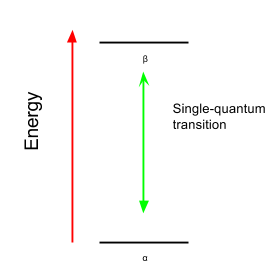
\includegraphics[scale=0.5]{figures/one_spin_1-2}
  \caption{An energy-level diagram for a spin system of a single nucleus.}
  \label{one_spin_1-2}
\end{figure}

\begin{figure}[h]
  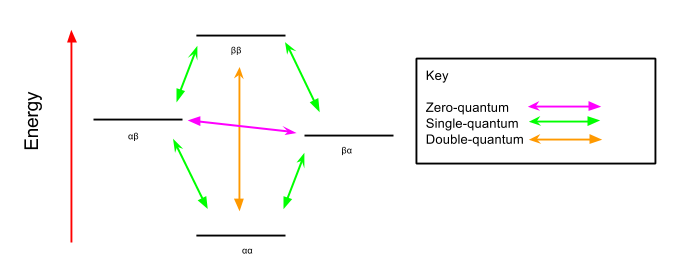
\includegraphics[scale=0.5]{figures/two_spins_1-2}
  \caption{An energy-level diagram for a spin system containing two nuclei.}
  \label{two_spins_1-2}
\end{figure}

\begin{figure}[h]
  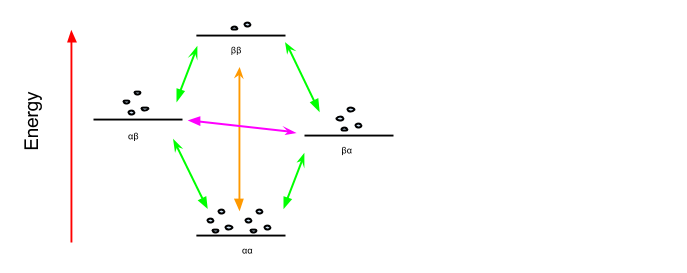
\includegraphics[scale=0.5]{figures/two_spins_initial}
  \caption{The initial population distribution of a two-spin system.}
  \label{two_spins_initial}
\end{figure}

\begin{figure}[h]
  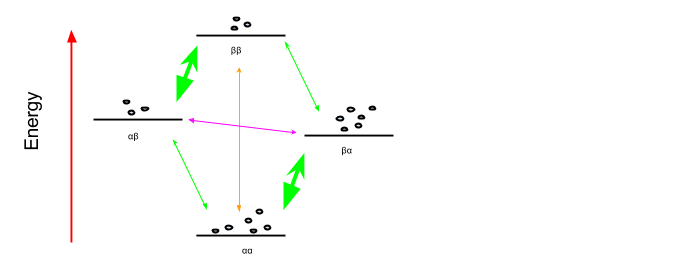
\includegraphics[scale=0.5]{figures/two_spins_rf}
  \caption{An RF pulse on one nucleus equalizes its populations.}
  \label{two_spins_rf}
\end{figure}

\begin{figure}[h]
  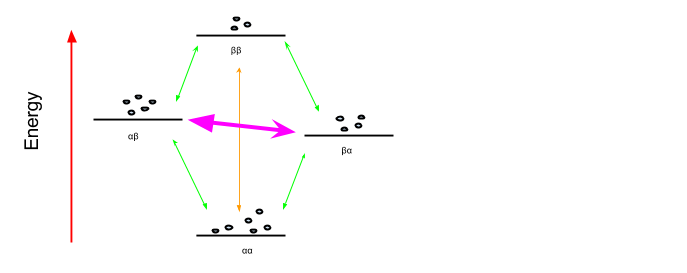
\includegraphics[scale=0.5]{figures/two_spins_w0}
  \caption{Relaxation in the case where the zero-quantum rate is faster.}
  \label{two_spins_w0}
\end{figure}

\begin{figure}[h]
  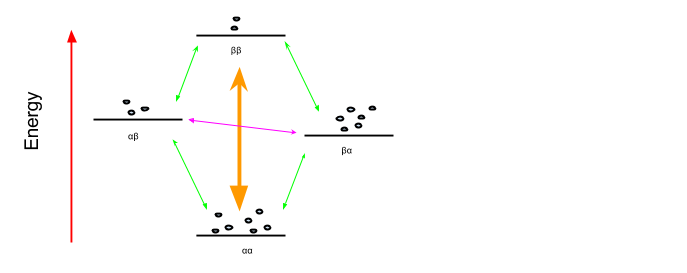
\includegraphics[scale=0.5]{figures/two_spins_w2}
  \caption{Relaxation in the case where the double-quantum rate is faster.}
  \label{two_spins_w2}
\end{figure}



\chapter{NMR Data Analysis is Irreproducible}

This chapter will describe the NMR data analysis process in detail,
including the roles of computational and manual analysis, as well as
the data and tools involved in the process.


\section{Time-domain Data Collection}

Time-domain NMR data, or FIDs, are collected by placing a concentrated
sample in a spectrometer, running various pulse sequences, and recording
the resultant data.  Pulse sequences \cite{khaneja2005} are designed to 
target specific nuclei, and the collected FIDs are sums of decaying sinusoids.

The collection of data suitable for Fourier Transform processing, described
in the next section, requires uniformly collected data in each dimension.
The delay between data points, number of points collected, and total delay
between the first and last point (or acquisition time, which may be calculated
from the first two parameters) determines the spectral width, or range of
different frequencies that can be distinguished, and resolution, or the
ability to distinguish nearby but distinct signals in the frequency domain
\cite{ernst2004}.

Sensitivity, which determines the ability to discern true signals
from noise in the frequency domain, places constraints on data collection
\cite{rovnyak2004accelerated}.  Non-uniform sampling approaches 
\cite{maciejewski2011random} avoid these tradeoffs by collecting more data
points where the signal-to-noise ratio is high, but maintain resolution by
still collecting some data points where the signal-to-noise is low.
However, it is important to capture the sample schedule used as well, since
it gives rise to frequency-domain artifacts according to its point spread
function.


\section{Spectral processing}

The raw data collected from an NMR spectrometer is referred to as 
time-domain data.  In a typical NMR experiment, these data represent the 
sum of multiple decaying sinusoids.  These FIDs are converted to 
frequency-domain spectra which are used in further analysis.  The goal of 
this phase is to construct a frequency spectrum which indicates the resonance 
frequencies of the atoms that were observed in the experiment.  A common tool 
for such a transformation is the Fourier Transform, which is able to convert 
a uniformly collected data set into a frequency spectrum.  
An example of an NMR spectrum of N-H groups is shown in Figure-\ref{nhsqc}.
Due to relaxation decreasing the amplitude of an NMR signal over time, peaks 
have an intrinsic linewidth in the frequency spectrum.

Alternative approaches include multidimensional decompsition \cite{mdd}
and maximum entropy reconstruction \cite{hoch1996nmr}.  When FIDs are 
non-uniformly collected, these processing methods are required.

Considerations include minimization of processing artifacts, signal-to-noise 
ratio, accounting for water lines, avoiding rolling baselines and baseline 
offsets, linewidth and shape, phasing, and apodization.  Multiple software 
packages exist for carrying out this conversion \cite{nmrpipe, rnmrtk}.
These packages include functions for processing the data in specific ways to 
guarantee desirable qualities.  A typical procedure for spectral processing 
involves the sequential application of multiple functions from one of these 
packages.  At each stage, the input is a data set and associated metadata, 
which includes information such as spectral width, dwell time, and number of 
points.  Each function may require the setting of one or more parameters in 
order to proceed.  Thus, in addition to the final frequency-domain spectrum, 
the process to create generates several intermediate data sets, several 
intermediate metadata sets, and the sequence of functions used along with 
their parameterizations.  Previous work from our lab has enabled the 
convenient collection of necessary metadata during spectral 
processing \cite{connjur-wb}.


\section{Peak picking}

The Fourier Transform of a decaying sinusoid produces a frequency-domain 
spectrum with a peak at a frequency matching the oscillation frequency of 
the sinusoid.  Since NMR time-domain data consists of multiple decaying 
sinusoids caused by atoms resonating at characteristic chemical shifts, 
the frequency domain spectrum will contain peaks for every oscillating 
sinusoid present in the time-domain data.  
Peak picking involves identification of the peaks, including their
chemical shift frequencies, shape, intensity, and width.  

In general, a peak is a local maximum in the frequency spectrum.  However,
not all local maxima are necessarily peaks due to noise and artifacts.
Nor do all peaks show up as local maxima if they are weak and close to the noise
level, which causes them 
to be nearly indistinguishable from the noise and baseline; this may be due to 
sample instability such as aggregation or precipitation, or low sample 
concentration \cite{picky, munin, korzhnev2001munin, apart, autopsy, pine}
\cite{williamson2009automated, guntert2009automated, altieri2004automation,
baran2004automated}.
Since peaks have non-zero widths, peaks that are closer than their
widths will overlap, distorting measurement of their attributes and possibly
also leading to disappearance of a local maximum.  These issues complicate peak 
picking, the goal of which is to find all true signal peaks and only true 
signal peaks.
Figure-\ref{nhsqc_peaks} shows a portion of a peak-picked
NHSQC spectrum; note the overlap between some peaks, and that some -- but not
all -- low-intensity spectral features have been identified as peaks.

Given these inherent issues, a general strategy for peak picking is 
described in \cite{autopsy, picky}.
First, the noise level is estimated and points below the noise are discarded.
Next, of the remaining spectral regions, isolated areas are picked as peaks.
Finally, overlap is resolved by lineshape matching and the peaks are picked
and their attributes measured.  An optional additional step is filtering
based on symmetry and linewidth \cite{autopsy, picky}.

Correct peaks are important because they form the basis for the construction 
of GSSs, the assignment of chemical shifts to atoms, and the interpretation of 
NOESY spectra which give rise to distance restraints as a preliminary to 
structure calculation \cite{guerry2011automated}.  
Incorrect peak identification or position can result 
in misinterpretation of NOESY spectra, which could lead to false distance 
restraints between atoms which are in fact very far apart in the actual 
protein structure.

Estimates of the amount of false positive and false negative peaks picked 
by computational tools range from very low (10-40\%) to very high (70-135\%) 
\cite{pine}. 
The quality of the results generally depends on characteristics of the 
spectrum, especially the signal/noise ratio, and resolution, as well as 
characteristics of the molecule including T\textsubscript{2} (which has an 
effect on peak width) and number of atoms -- the issue being that more atoms 
means more peaks, which means a higher chance of overlap.

Since none of these approaches yields perfect 
results \cite{guerry2011automated}, manual intervention during peak picking 
is important for obtaining results of sufficiently high quality
\cite{guntert2009automated}; many peak picking 
programs allow and encourage semi-automated interaction in order to clear 
up troublesome spectral features.  
Manual intervention is often accomplished based on knowledge outside of the 
spectrum: existence, position, and shape of peaks in other spectra, knowledge 
of the solvent, characteristic artifactual patterns caused by a specific 
processing scheme, knowledge of the local dynamics of a small region of the 
protein.  \cite{williamson2009automated, guntert2009automated, 
altieri2004automation, baran2004automated}
Because of this, peak picking can often not be completely finished until 
later analysis has been accomplished.


\section{GSSs and resonances}

GSSs \cite{saga, ezassign, pistachio, autoassign1997, autoassign2001}
and resonances \cite{ccpn} are parallel to residues and atoms.
They are key to data analysis because they are the link between what is 
observed in NMR experiments and the molecular details of the sample.
Although these concepts had been used to a limited extent by earlier programs
\cite{xeasy, sparky}, more recent work has treated GSSs and resonances as 
explicit, first-class members of data analysis \cite{ccpn, bmrb}.

\subsection{Resonances}
A resonance is an NMR-visible signal which corresponds to an atom \cite{ccpn}.
In general, an atom resonates at a single characteristic frequency based
on its local environment;  the same resonance will be found at the same 
frequency across multiple experiments.  This phenomenon is used to aid in 
identification, although it is confounded by degeneracy as well as proteins
with multiple conformations.

\subsection{GSSs}
A GSS is an NMR-visible group of peaks, typically across multiple spectra,
which corresponds to a group of covalently bonded resonances; it is similar
to a residue.  
The key to GSSs is a battery of multi-dimensional pulse 
sequences designed to correlate resonances within GSSs 
\cite{cavanagh1995protein, hncacb, hnco, cbcaconh}.  These experiments are all
based on an N-H group (due to its sensitivity and chemical shift dispersion)
and correlate additional nearby nuclei through covalent bonds.

These pulse sequences use several types of overlap.  First, each pulse sequence
includes the N-H group.  Second, due to the similar scalar couplings between
N and the CA and CA(i-1) nuclei, it is possible to simultaneously correlate an
N-H group with both nearby CA nuclei; this means that each CA may be correlated
with two N-H groups, or in other words, may be a part of two GSSs. 
Third, due to the scalar coupling between N and CO(i-1), correlations to 
C*(i-1) appear in two pulse sequences of a pair (e.g. HNCACB and CBCA(CO)NH), 
while C* appear in only the HNCACB.  See Figure-\ref{ccpn_nhsqc}, 
Figure-\ref{ccpn_hncacb}, Figure-\ref{ccpn_cbcaconh}, Figure-\ref{ccpn_hnco}, 
Figure-\ref{ccpn_hncaco} for an illustration of the correlated nuclei.

These characteristics lead to a natural definition of a GSS: a root 
resonance or resonances, typically an amide H-N group, and additional 
covalently-bonded resonances.  The precise extent of a GSS is in principle 
determined by the available NMR experiments \cite{hncacb, hnco, cbcaconh}.  
In practice, a backbone GSS often is initially 
comprised of a backbone H-N, CO, CA, CB, CO(i-1), CA(i-1), and CB(i-1).  


\section{GSS and resonance construction}

This H-N matching enables grouping of peaks into GSSs; given multiple spectra
which include N-H dimensions, peaks with matching N and H chemical shifts are
determined to belong to the same GSS.
Table-\ref{pulse_sequences} shows that H-N chemical shifts are captured in 
multiple spectra, and sometimes multiple times within a single spectrum.
At a later stage, GSSs are often augmented with additional sidechain resonances.
	
In addition to GSSs of backbone resonances, H-N-rooted GSSs typically are 
visible for Asparagine and Glutamine sidechains, and smaller GSSs of 
Tryptophan sidechains are visible.  Arginine sidechains may also give rise 
to an H-N-rooted GSS under certain experimental conditions. 

The difficulty in constructing these GSSs correctly and unambiguously stems 
from the issues inherent in NMR data.  First, the success of the standard 
suite of experiments rooted in H-N -- NHSQC, HNCO, HNCACB, etc. -- depends 
on \cite{autoassign1997}: % page 600 -- `reliability`
\begin{enumerate}
  \item good dispersion, i.e. no overlap, otherwise it is difficult to determine 
    which peaks belong with which H-N-rooted spin system.
  \item the H-N chemical shifts being nearly identical across all spectra.  
    This may not be the case if there are variations in the sample or the 
    temperature.  The Block-Siegert shift and experimental error also can have 
    an effect on chemical shift.
  \item nuclei appearing at a single chemical shift.  If there are multiple 
    conformations or chemical heterogeneity \cite{autoassign1997}, 
    a nucleus may appear at multiple chemical shifts and appear to be two 
    different resonances.
  \item the presence of an H-N group -- Proline is a notable exception, and 
    so it does not show up in experiments which rely on the presence of an H-N group
  \item extraneous peaks which do not seem to fit into a spin system, or 
    peaks which do not seem to match peaks in other spectra
  \item accurate (or at least consistent) spectral referencing.  
    Misreferenced spectra will cause the same nucleus to show up at different 
    chemical shifts across multiple spectra.
  \item quality of peak-picking \cite{autoassign1997, mars}: 
    chemical shifts, lineshapes, as well as the numbers of 
    false positives, false negatives, extraneous peaks
\end{enumerate}

Computational approaches for GSS construction tend to require manual 
assistance in some cases \cite{autoassign1997, mars}.  Incorrect or 
incomplete GSSs will have negative effects on the quality of later 
analysis; several assignment tools assume that manual intervention will 
verify and, if necessary, correct the GSSs \cite{williamson2009automated}; 
this allows the tools to be conservative in their 
predictions \cite{autoassign1997}.  However, it may not be 
possible to unambiguously and completely construct GSSs until the results 
of later analysis are available: some approaches use NOESY peaks and 
assignments as well as structure results to verify and correct GSSs 
\cite{autoassign1997}.

Figure-\ref{nhsqc_hncacb} shows an example of matching peaks between two
spectra.  The quality of the match -- how closely the chemical shifts line up,
as well as the lack of overlapping peaks -- means the peaks are easily
identified as members of the same GSS.


\section{Backbone spin systems and resonances: typing and sequence-specific assignment}

Once GSSs have been constructed, analysis continues with four simultaneous 
assignment subtasks: resonance typing, GSS typing, GSS to
GSS sequentially, and GSS to specific residues of the sample of interest.

\subsection{Assignment of resonance to atomtype}

Before assigning a resonance to a specific 
atom, the atomtype of a resonance may be assigned.  In an HNCO experiment, 
this is typically straightforward, because for each backbone spin system, 
the H dimension always corresponds to the backbone H, the N dimension always 
corresponds to the backbone N, and the C dimension always corresponds to the 
backbone C(i-1).  However, the situation is more complicated in an HNCACB 
experiment, as there are generally four choices of atomtype assignment for 
the C dimension:  CA, CB, CA(i-1), and CB(i-1).  Thus, the resonance given 
by the C dimension of each peak must be assigned one of these choices.  
Reasons for choosing a specific assignment include peak sign, as well as 
chemical shift compared to statistics available in the BMRB.  In addition, 
the overlap between experiment pairs such as the HNCACB and CBCA(CO)NH 
facilitates resonance-atomtype assignment: while the CA(i-1) and CB(i-1) 
are expected to appear in both experiments at the same chemical shift for 
a given backbone H-N root, the CA and CB are expected to appear only in the 
HNCACB spectrum.

\subsection{Assignment of amino acid type to GSS}

Correspondingly, GSSs are also assigned amino acid types.  This phase 
interacts strongly with the assignment of atomtypes to resonances, in 
that the possible atomtypes to which a resonance may be assigned depends 
on the amino acid type, and the expected chemical shift ranges for various 
atomtypes depends on amino acid type as well.  For instance, GSSs assigned 
to the Glycine amino acid type should not have a CB; and the CB resonance's 
chemical shift of a GSS assigned to Alanine is expected to be very different 
from all other CB chemical shifts.  Backbone amino acid types may be split 
into several categories \cite{saga} based on BMRB statistics for 
CA and CB chemical shifts \cite{bmrb}:
\begin{enumerate}
  \item Ala
  \item Gly 
  \item Pro
  \item Ser, Thr
  \item Val, Met, Lys, His, Arg, Glu, Gln, Trp, Cys
  \item Asp, Asn, Ile, Leu, Phe, Tyr
\end{enumerate}
However, GSS typings are complicated by several factors.  First, GSS typing 
requires correct and complete GSS construction.  Second, correctly assembled 
GSSs may include overlapped or extraneous peaks, expected peaks (based on a 
spectrum's typical results) may also be missing.  Third, most GSSs can not 
be uniquely typed based solely on CA and CB chemical shifts, as groups 5 and 
6 (above) as well as 4 are ambiguous.  Fourth, sidechain GSSs must be 
identified and separated.

\subsection{Assignment of GSS to GSS sequentially}

Sequential GSS assignments exploit the previously mentioned overlap of pulse
sequences such as the HNCACB and HN(CA)CO.  Sequential GSSs 
are expected to have CA/CA(i-1), CB/CB(i-1), and CO/CO(i-1) resonances at 
identical chemical shifts.  This duplication enables sequential assignment 
of GSSs.  Note that there is substantial interaction between atomtype-resonance 
assignment and sequential GSS assignment: assigning two GSSs sequentially 
implies the CB vs CB(i-1), CA vs CA(i-1), and C vs C(i-1) atomtype assignments 
of the resonances in both GSSs; knowing the atomtype-resonance assignments of 
two spin systems can prevent their sequential assignment (if, for example, the 
matching resonances are both CB(i-1)); and not knowing the atomtype-resonance 
assignment implies that the sequential GSS assignment may be invalid.  
Sequential GSS assignment is complicated by: 
\begin{enumerate}
  \item missing peaks, possibly caused 
  by local dynamics, which reduce the number of overlapping resonances between 
  potential sequential GSSs, and can also disrupt atomtype assignments of 
  resonances; 
  \item extraneous peaks, which may be false positives or caused by 
  multiple conformations of the protein, causing incorrect matches
  \item degeneracy of chemical shifts:  given two GSSs with identical CA(i-1) 
  and CB(i-1) resonances, as well as a third GSS with matching CA and CB 
  resonances, it is impossible to unambiguously assign sequentially solely 
  on the basis of chemical shift matching between the two GSSs 
  \cite{autoassign1997}.
\end{enumerate}

An example of GSS overlap is shown in Figure-\ref{hncacb_overlap}.  Green peaks
are CA, and purple peaks are CB; note that one each of green and purple peaks
match between the two GSSs.

\subsection{Assignment of GSS to specific residue of sample of interest}

The final piece of backbone analysis is assignment of GSSs to specific 
residues.  Since backbone GSSs are H-N-rooted, a GSS is assigned to a 
backbone-amide; this implies the assignment of resonances to atoms as well, 
based on matching of atomtypes.  When a typical GSS is assigned to a residue, 
the H, N, C, C(i-1), CA, CA(i-1), CB, and CB(i-1) atoms will be assigned 
resonances as well.  Sequence-specific assignment interacts heavily with 
sequential GSS assignment, because the protein sequence must be compatible 
with the GSS sequence, where `compatible' means that the amino acid types 
of the GSS match those of the protein sequence.  Note that full assignment 
of amino acid type to GSS is not a prerequisite for GSS-residue assignment; 
in fact, GSS-residue assignment may lead to GSS-amino acid type assignment 
for sequentially connected GSSs.  GSS-residue assignment is facilitated by 
long chains of sequential GSSs in which some of the GSSs are typed as Serine, 
Threonine, Glycine, or Alanine.  The longer a GSS chain, the fewer places it 
might possibly fit into the protein sequence \cite{saga}.  Also, 
as sequence-specific assignment proceeds, the number of unassigned GSSs and 
residues decreases; the result is that initially ambiguous assignments become 
unambiguous as choices are removed.  Conversely, complications arise from 
incomplete sequential GSS assignments resulting in short, ambiguous chains.  
The presence of prolines generally ends chains due to the lack of a backbone 
H-N group.  Missing GSSs also terminate chains.  Relatively few Ser, Thr, Gly, 
and Ala residues means the number of unambiguous anchor points will be lower.

Figure-\ref{ss-residue} shows an example of sequence-specific GSS assignment.
Although not all of the GSSs have been typed, the presence of a Glycine and
Serine in the GSS chain reduces the possible assignments to residues.
Additionally, the length of the GSS chain helps reduce the ambiguity compared
to shorter GSS chains.


\section{Sidechain: spin system and resonance assignment}

The next group of experiments collects chemical shifts of sidechain atoms.  
These experiments include 
the HBHA(CO)NH \cite{hbhaconh} in Figure-\ref{ccpn_hbhaconh}, 
the C(CO)NH-Tocsy \cite{cconhtocsy} in Figure-\ref{ccpn_cconhtocsy}, 
the HC(CO)NH-Tocsy \cite{hcconhtocsy} in Figure-\ref{ccpn_hcconhtocsy}, 
the HCCH-Tocsy \cite{hcchtocsy} in Figure-\ref{ccpn_hcchtocsy}, 
and aromatic Tocsys.  The purpose of these experiments is to 
obtain the chemical shift values of sidechain resonances of protons, since 
proton frequencies are necessary in order to interpret NOESY spectra.  To 
interpret these spectra, the peaks must be assigned to GSSs and atomtypes 
must be assigned to the new resonances. While several of these experiments 
are also rooted in backbone H-N groups, facilitating the addition of peaks 
to the correct GSS, others -- such as the HCCH-Tocsy -- are not.  These are 
analyzed by the matching of resonance chemical shifts with those from other 
experiments targeting sidechains.  Atomtype-resonance assignments can generally 
be made with reference to compiled BMRB statistics.  Complications in this 
phase include: stereospecificity -- nuclei such as HA2 and HA3 may give rise 
to different chemical shifts, but resolving the correspondence may be 
impossible without further data; overlap -- especially in the HCCH-Tocsy 
where sidechains of the same amino acid type but different residue may have 
many closing matching chemical shifts; overlap between resonances within the 
same GSS, especially in Leu and Ile; missing and extraneous data; and the 
difficulty of both obtaining and unambiguously interpreting aromatic data.  
New approaches for sidechain data collection and assignment have recently 
been developed \cite{mobli2010non, hiller2008apsy} which seek to address 
these issues by reducing ambiguity of chemical shifts.


\section{Alternative approach: probabilistic assignment}

The previously described approach views analysis as a pipeline: input is 
transformed into output, which becomes the input for the next stage, and so on.  
PINE \cite{pine} removes the pipeline constraint by connecting each stage to 
each other and allowing information to flow freely; this enables statistical 
weighting of interpretation as well as dependencies such as peak picking 
on GSS construction (a dependency which is not possible in the pipeline 
approach).  PINE does not remove the need for manual intervention; it is
still assumed that some level of intervention is necessary to obtain the
best results \cite{pine}.


\section{NOESY peak-picking and assignment}

In NOESY spectra, each true peak indicates a pair of protons within 
approximately 5 Angstroms of each other.  This is different from the 
correlation spectra discussed earlier, in which peaks indicate covalently 
bonded atoms; NOESY spectra do not depend on covalent bonds but rather 
depend on spatial proximity.  Thus, each NOESY peak contains some information 
about the actual three-dimensional structure of a molecule, if it can be 
determined which protons give rise to the peak.  Analysis of NOESY spectra 
requires chemical shift assignments of atoms, and uses that information to 
determine the protons involved in a peak.  Considerations used to analyze 
NOESY spectra include: symmetry -- a peak is expected to correspond to a 
matching peak with the frequencies of the two 1H dimensions swapped; patterns 
based on known proximity of atoms from the primary sequence giving rise to 
many short-distance NOE peaks; network anchoring.  Complications include 
overlap caused by degenerate chemical shifts of protons, leading to 
ambiguous interpretations of peak assignments; this can be greatly mitigated 
by the use of an extra dimension:  15N- or 13C-edited NOESY spectra reduce 
the ambiguity, as well as incorrect or incomplete chemical shift assignments.

NOESY assignment is generally done automatically \cite{cyana2004, aria2003}.  
NOESY peak-picking may be automated as well \cite{munin, korzhnev2001munin}.

An alternative approach is taken by ABACUS \cite{abacus_assignment}, which uses
Monte Carlo probabilistic methods for assignment, NOE assignment, and structure
calculation.  However, it is important to note that ABACUS still requires 
correct NOE peak picking and GSS construction as a prerequisite.


\section{Structure calculation}

Cyana is able to calculate a three-dimensional structure from NOESY peaks, 
chemical shift assignments, and distance restraints \cite{cyana2004, aria2003} 
using an iterative approach to NOESY peak assignment and building structural 
models.  It also requires secondary structure information as input, which can 
be calculated from chemical shift assignments using a program such as 
\cite{talos+}.  Chemical shift assignments may also be used to 
calculate potential structures \cite{cs-rosetta}.  Additional programs 
may be used to refine structures \cite{amber, xplor-nih}.  This phase 
generally does not require manual intervention.


\section{Discussion}

The inherent NMR issues of ambiguous, missing, and extraneous data cause 
problems throughout the entire analysis process.  Correctly dealing with 
these issues is difficult, but absolutely critical in order to obtain 
high-quality results \cite{williamson2009automated, guntert2009automated, 
altieri2004automation, baran2004automated}.  As yet, computational tools 
are not able to deal perfectly with these issues.  
Most tools have several basic limitations: 
\begin{enumerate}
  \item they require high-quality input in order to function correctly 
  \cite{saga, abacus_assignment, mars, autoassign2001, ezassign, pine, cyana2004}; 
  this input is generally assumed to have been manually prepared in order 
  to meet the stringent quality requirements of completeness and absence of 
  extraneous results
  \item even with high-quality input data, tools are not able to produce 
  perfect results 
  \item tools perform differently in different contexts, although 
  performance generally decreases as protein size increases and spectral quality 
  decreases
  \item manual verification and correction of the results is assumed, 
  even for tools that claim to be fully automated 
  \cite{williamson2009automated, guntert2009automated, altieri2004automation,
  baran2004automated}
\end{enumerate}

A key limitation of many analysis tools is the limited input data.  While
this simplifies the use of the tool in a simple pipeline, it may also lead
to reduced quality of results and explain the necessity of manual intervention:  
while the input data that a tool handles is limited, manual interventions can
make use of any additional information required to make specific deductions. 
Thus, PINE and related efforts  
are an exciting effort to loosen these artificial restrictions.  Initial 
results are promising, and show a marked improvement, although manual 
intervention is still assumed to be necessary in order to obtain the best 
results \cite{pine}.  Further tools such as \cite{shiftx2, cheshire}, 
which calculate chemical shifts from structure,  
bring additional information to bear, helping to validate assignments.

Another exciting development is the rise of probabilistic methods 
\cite{saga, pine}.  These methods reflect the reality that the 
confidence of a specific interpretation depends on the exact state of the 
data; in other words, an assignment which is 50\% confident given only an 
HNCA spectrum may become 90\% confident if an HN(CO)CA spectrum is added.  
The significance of this confidence level is that it enables easy tracking 
of ambiguous and/or low-confidence interpretations -- i.e. those that stand 
to benefit from collecting additional data sets.  By including confidence 
values on all assignments, an understanding of the troublesome areas is 
facilitated.  This helps to reduce the cost of cascading errors -- if the 
uncertainty is tracked as a confidence level, further interpretations based 
on a highly uncertain datum will also receive low confidence levels.  In 
addition, confidence levels are an alternative to the inherent balance 
between completeness and correctness -- it is no longer necessary to 
sacrifice one for the other \cite{autoassign2001, pine}.


\section{Conclusions}

Manual analysis plays a critical role in NMR data analysis, due to the inherent 
issues involved in analysis and to the large amount of information which must 
be brought to bear to solve difficult cases.  Although spectral processing, 
NOESY assignment, and structure calculation have been automated, peak-picking, 
GSS construction, and assignment of both resonances and GSSs have not been 
completely automated.  Manual intervention is assumed to be necessary by 
most tools, even automated ones, to ensure the completeness and correctness 
of results.  However, despite the importance that manual intervention plays 
in analysis, the specific modifications made and their reasons for -- 
which may be quite complicated -- are not captured \cite{guntert2009automated}.  
Thus, the metadata of manual intervention is lost, and analysis is 
irreproducible.


% tables
\clearpage
\section{Tables}

\begin{table}[h] % if I don't add the [h], the table comes before the section title
    \begin{tabular}{ | c || c | c | c | c | c |}
    \hline
              & NHSQC & HNCO & HN(CA)CO & HNCACB & CBCA(CO)NH \\
    \hline
      H       & 1 & 1 & 2 & 4 & 2 \\
    \hline
      N       & 1 & 1 & 2 & 4 & 2 \\
    \hline
      CO      & 0 & 1 & 0 & 0 & 0 \\
    \hline
      CO(i-1) & 0 & 1 & 1 & 0 & 0 \\
    \hline
      CA      & 0 & 0 & 0 & 1 & 0 \\
    \hline
      CA(i-1) & 0 & 0 & 0 & 1 & 1 \\
    \hline
      CB      & 0 & 0 & 0 & 1 & 0 \\
    \hline
      CB(i-1) & 0 & 0 & 0 & 1 & 1 \\
    \hline
    \end{tabular}
    \caption{The number of times nuclei typically appear in pulse sequences}
    \label{pulse_sequences}
\end{table}


% figures
\clearpage
\section{Figures}

\begin{figure}[h]
  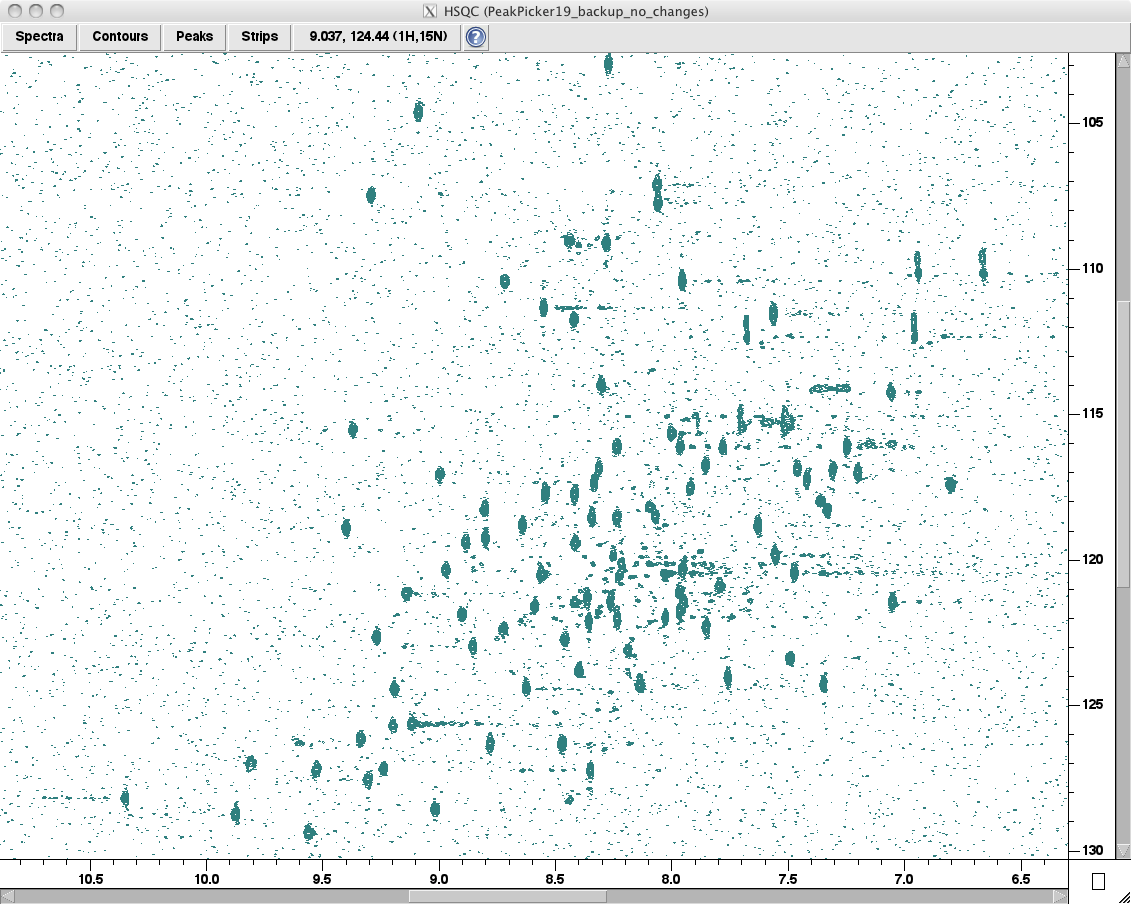
\includegraphics[scale=0.35]{figures/nhsqc}
  \caption[A frequency-domain NHSQC spectrum]
          {A frequency-domain NHSQC spectrum. 
           The x- and y-axes are nitrogen and proton, respectively.}
  \label{nhsqc}
\end{figure}

\begin{figure}
  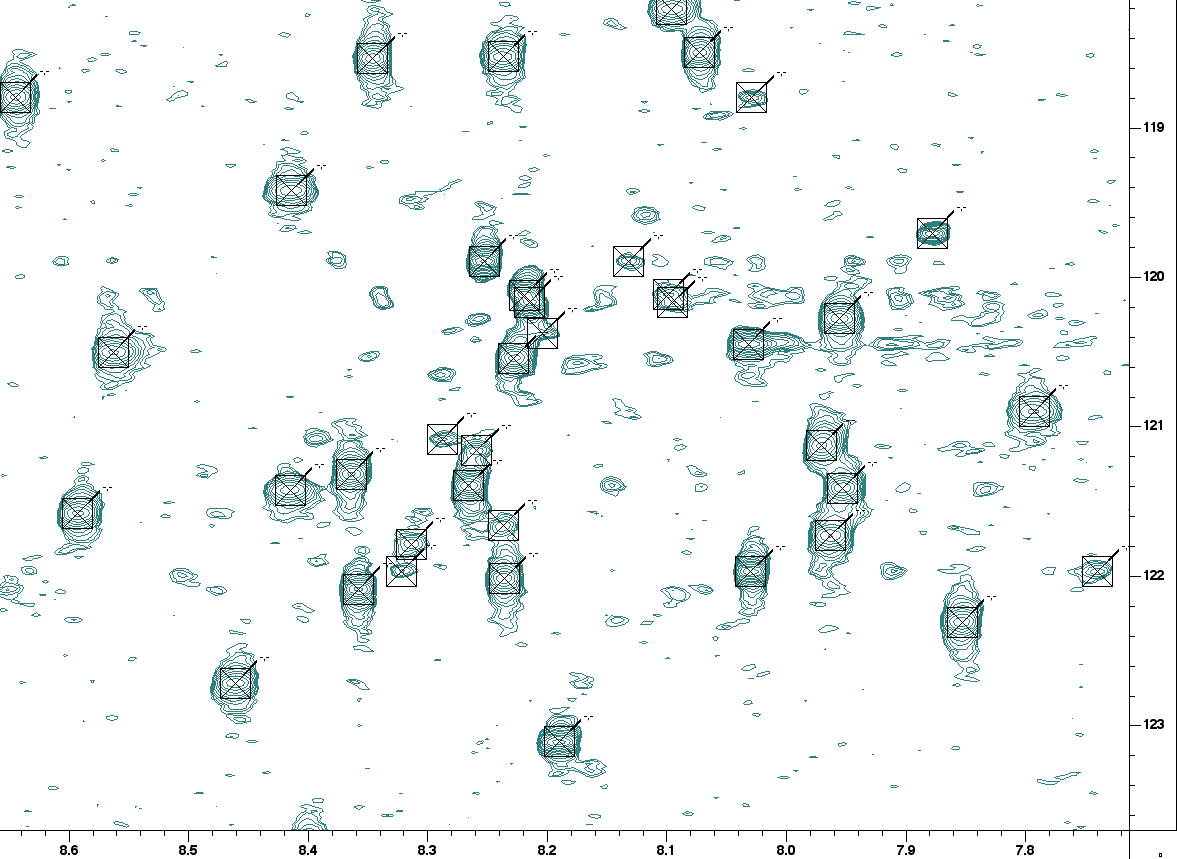
\includegraphics[scale=0.35]{figures/nhsqc_peaks}
  \caption[A peak-picked NHSQC spectrum]
          {A peak-picked NHSQC spectrum. 
           Peaks are indicated by black squares and crosses.}
  \label{nhsqc_peaks}
\end{figure}

\begin{figure}
  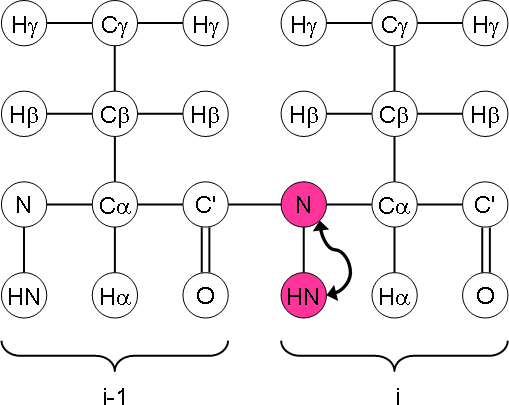
\includegraphics[scale=0.75]{figures/ccpn_nhsqc}
  \caption[The nuclei correlated by an NHSQC.]
          {The nuclei correlated (red) by an NHSQC.
           This figure is reproduced from \url{http://www.protein-nmr.org.uk/}
           with the permission of Victoria Higman.}
  \label{ccpn_nhsqc}
\end{figure}

\begin{figure}
  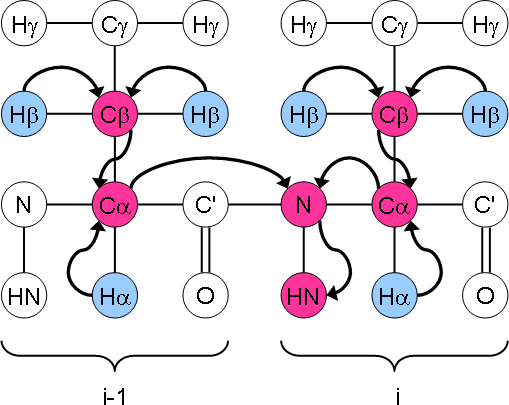
\includegraphics[scale=0.75]{figures/ccpn_hncacb}
  \caption[The nuclei correlated by an HNCACB.]
          {The nuclei correlated (red) by an HNCACB.
           This figure is reproduced from \url{http://www.protein-nmr.org.uk/}
           with the permission of Victoria Higman.}
  \label{ccpn_hncacb}
\end{figure}

\begin{figure}
  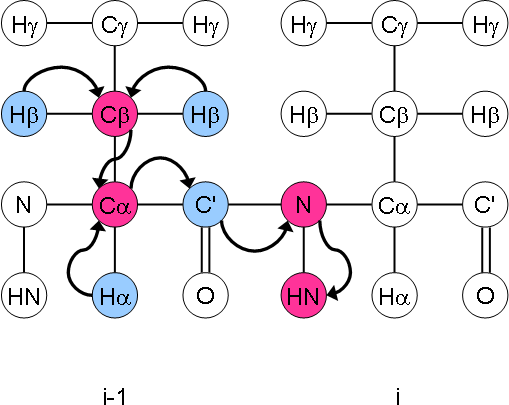
\includegraphics[scale=0.75]{figures/ccpn_cbcaconh}
  \caption[The nuclei correlated by a CBCA(CO)NH.]
          {The nuclei correlated (red) by a CBCA(CO)NH.
           This figure is reproduced from \url{http://www.protein-nmr.org.uk/}
           with the permission of Victoria Higman.}
  \label{ccpn_cbcaconh}
\end{figure}

\begin{figure}
  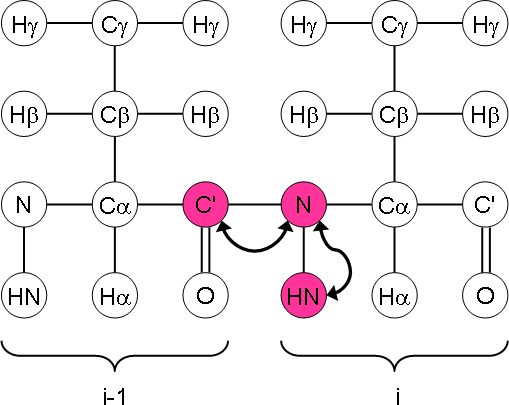
\includegraphics[scale=0.75]{figures/ccpn_hnco}
  \caption[The nuclei correlated by an HNCO.]
          {The nuclei correlated (red) by an HNCO.
           This figure is reproduced from \url{http://www.protein-nmr.org.uk/}
           with the permission of Victoria Higman.}
  \label{ccpn_hnco}
\end{figure}

\begin{figure}
  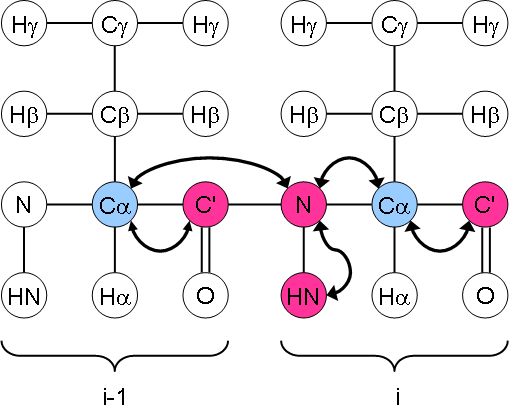
\includegraphics[scale=0.75]{figures/ccpn_hncaco}
  \caption[The nuclei correlated by an HN(CA)CO.]
          {The nuclei correlated (red) by an HN(CA)CO.
           This figure is reproduced from \url{http://www.protein-nmr.org.uk/}
           with the permission of Victoria Higman.}
  \label{ccpn_hncaco}
\end{figure}

\begin{figure}
  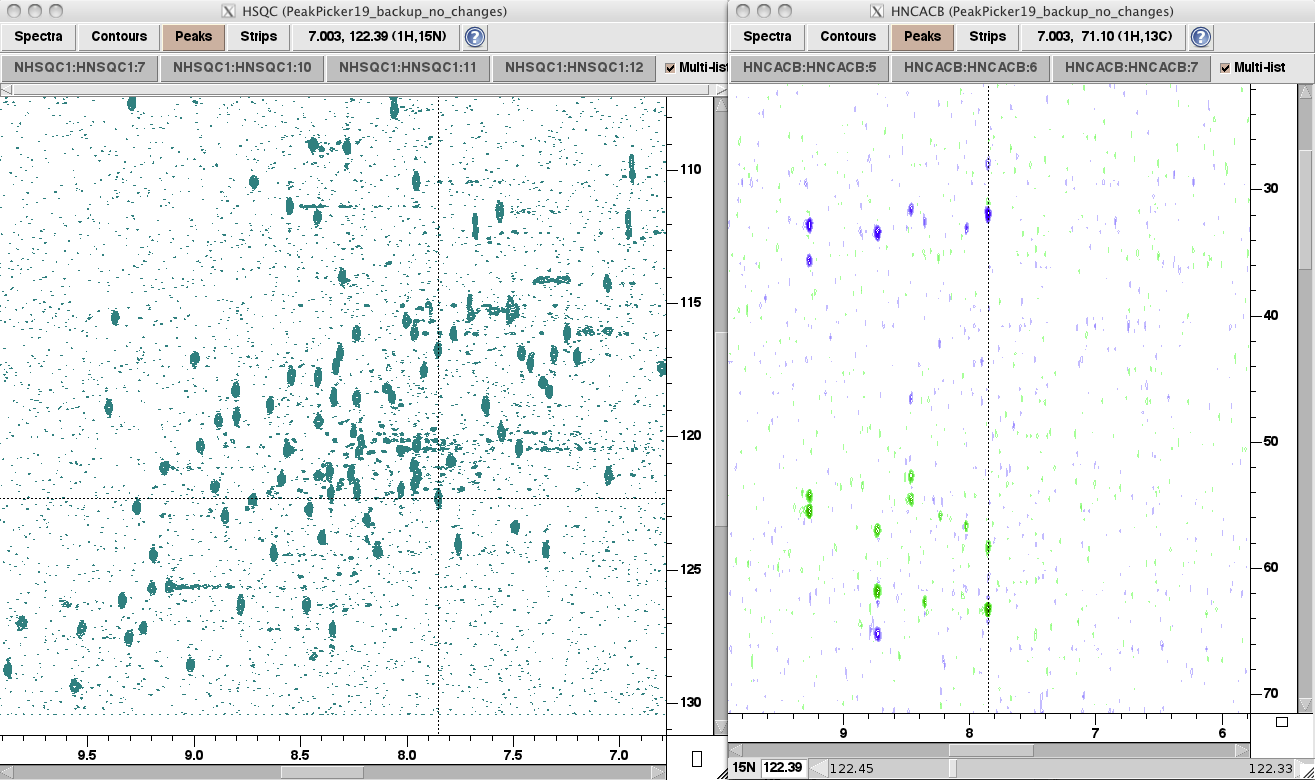
\includegraphics[scale=0.3]{figures/nhsqc_hncacb}
  \caption[Matching peaks between an NHSQC and an HNCACB spectrum]
          {Matching peaks between an NHSQC and an HNCACB spectrum.
           This likely indicates that the peaks belong to the same GSS.}
  \label{nhsqc_hncacb}
\end{figure}

\begin{figure}
  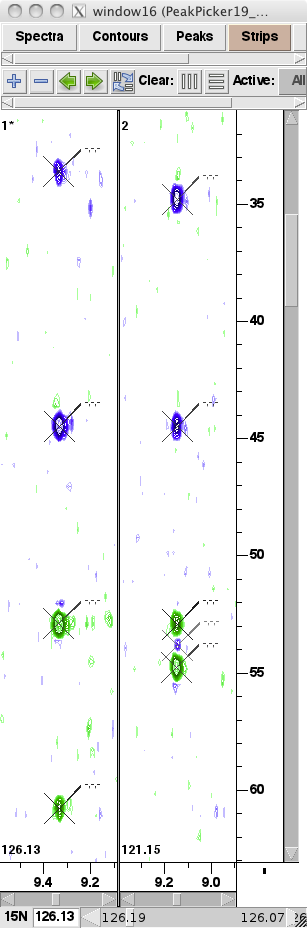
\includegraphics[scale=0.35]{figures/hncacb_overlap}
  \caption{Overlap of Carbon resonances in an HNCACB spectrum.}
  \label{hncacb_overlap}
\end{figure}

\begin{figure}
  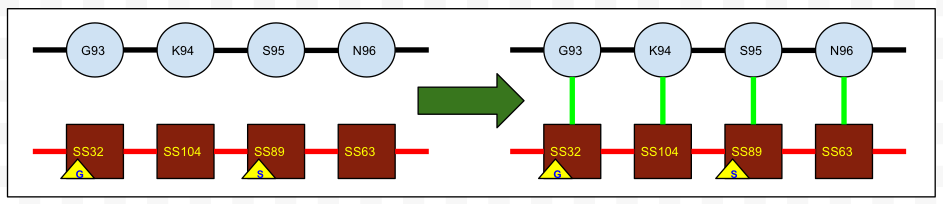
\includegraphics[scale=0.45]{figures/ss-residue}
  \caption[Assignment of a GSS chain to residues]
          {Assignment of a GSS chain to residues.  The circles are residues,
           black lines are peptide bonds, squares are GSSs, red lines are 
           sequential GSS assignments, and green lines are GSS-residue 
           assignments.}
  \label{ss-residue}
\end{figure}

\begin{figure}
  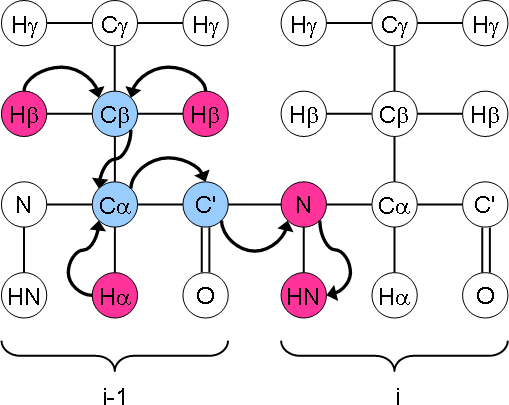
\includegraphics[scale=0.75]{figures/ccpn_hbhaconh}
  \caption[The nuclei correlated by an HBHA(CO)NH.]
          {The nuclei correlated (red) by an HBHA(CO)NH.
           This figure is reproduced from \url{http://www.protein-nmr.org.uk/}
           with the permission of Victoria Higman.}
  \label{ccpn_hbhaconh}
\end{figure}

\begin{figure}
  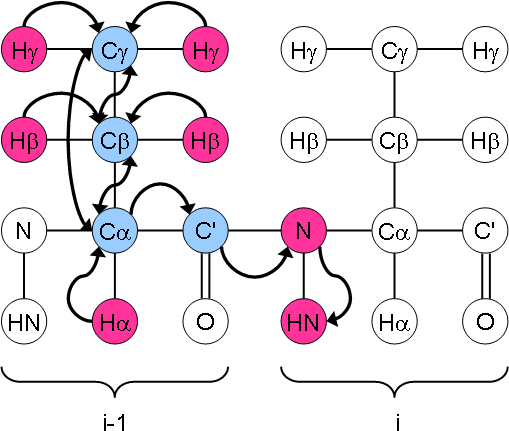
\includegraphics[scale=0.75]{figures/ccpn_hcconhtocsy}
  \caption[The nuclei correlated by an H(CCO)NH-Tocsy.]
          {The nuclei correlated (red) by an H(CCO)NH-Tocsy.
           This figure is reproduced from \url{http://www.protein-nmr.org.uk/}
           with the permission of Victoria Higman.}
  \label{ccpn_hcconhtocsy}
\end{figure}

\begin{figure}
  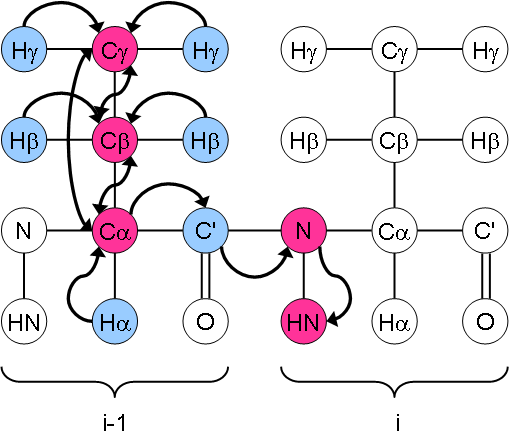
\includegraphics[scale=0.75]{figures/ccpn_cconhtocsy}
  \caption[The nuclei correlated by a C(CO)NH-Tocsy.]
          {The nuclei correlated (red) by a C(CO)NH-Tocsy.
           This figure is reproduced from \url{http://www.protein-nmr.org.uk/}
           with the permission of Victoria Higman.}
  \label{ccpn_cconhtocsy}
\end{figure}

\begin{figure}
  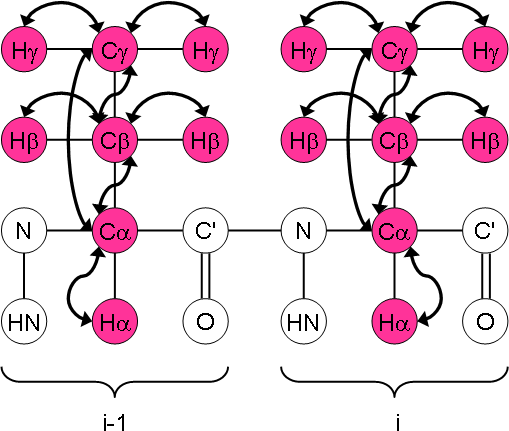
\includegraphics[scale=0.75]{figures/ccpn_hcchtocsy}
  \caption[The nuclei correlated by an HCCH-Tocsy.]
          {The nuclei correlated (red) by an HCCH-Tocsy.
           This figure is reproduced from \url{http://www.protein-nmr.org.uk/}
           with the permission of Victoria Higman.}
  \label{ccpn_hcchtocsy}
\end{figure}



\chapter{A Data Overview}
\label{ch_data_overview}

\begin{center}
  \textit{With insufficient data it is easy to go wrong.}

 - Carl Sagan
\end{center}

NMR data can be broadly grouped into four categories based on when it
is known.  First, Figure \ref{data_overview_1}, 
there is information that is known without performing
any NMR experiments: this includes information about the molecule as well
as general NMR and molecular knowledge.  Second,
Figure \ref{data_overview_2}, is data that is 
collected using the NMR spectrometer, and is known before analysis begins.  
Third, Figure \ref{data_overview_3}, is the information generated during 
analysis, and fourth, Figure \ref{data_overview_4}, is the final goal of 
an NMR study, information about the actual structure of the molecule of 
interest.

This chapter will present the data generated during the NMR process.
Later chapters will focus in on subsets of the data, as well as show how
the data is used during analysis.


\section{Global prior knowledge}
Knowledge of NMR and molecules that is available before any experiments are
performed.

\subsection*{Molecule}

\subsubsection{Primary sequence}
The primary sequence of amino acids -- for example, the sequence of Ubiquitin
is MQIFVKTLTG KTITLEVEPS DTIENVKAKI QDKEGIPPDQ QRLIFAGKQL EDGRTLSDYN IQKESTLHLV LRLRGG
according to Swiss-Prot -- of the protein is known.  

\subsubsection{Amino acids}
The atoms contained in each amino acid (see Table \ref{alanine_atoms}), 
bond lengths between atom pairs (see Table \ref{alanine_bond_lengths}), 
and bond angles (see Table \ref{alanine_bond_angles}) are known 
\cite{alanine_sreepad}.

\subsection*{NMR}

\subsubsection{Nuclei}
The gyromagnetic ratio of nuclei (see Table \ref{gyromagnetic_ratios}) and 
pulse sequences.  The gyromagnetic ratio and the magnetic field strength 
determine the approximate frequency range at which nuclei appear in spectra.

\subsubsection{Time-domain data}
Resonances appear as decaying sinusoids, and the full data set is a sum of
many of those sinusoids at varyious frequencies and intensities.
This is exploited in transforming time-domain data sets to frequency-domain.

\subsubsection{Through-bond experiments}
Time-domain free induction decay (FID)s are collected using
pulse sequences \cite{khaneja2005} designed to target specific nuclei by
exploiting the coupling constants and characteristic chemical shifts of specific 
nuclei and functional groups.  The collected FIDs are sums of decaying sinusoids.

The pulse sequence determines which covalently bound groups will appear in 
experiments (see Tables \ref{nhsqc_peaktypes}, \ref{hnco_peaktypes}, 
\ref{hncacb_peaktypes}, \ref{hbhaconh_peaktypes}, \ref{cconh_peaktypes}, and
\ref{hcconh_peaktypes}).

\subsubsection{Through-space experiments}
Nuclear Overhauser Effect (NOE) \cite{noe_kaiser} experiments transfer 
magnetization between spatially near proton pairs, and do not require a 
network of covalent bonds.  Each true peak indicates a pair of protons within 
approximately 5 Angstroms of each other.  This is different from 
through-bond correlation spectra, in which peaks indicate the nuclei of covalently 
bonded atoms; NOESY spectra do not depend on covalent bonds but rather 
depend on spatial proximity.  Thus, each NOESY peak contains some information 
about the actual three-dimensional structure of a molecule, although this
information is not used until the correspondence between peak cross
section and an atom's nucleus is determined.

\subsubsection{Resonance}
A particular nucleus is expected to resonate at approximately the same 
frequency in all spectra (although factors such as temperature and the 
Bloch-Siegert shift can produce differences).

\subsubsection{Frequency-domain spectra}
The Fourier Transform of a decaying sinusoid produces a frequency-domain 
spectrum with a peak at a frequency matching the oscillation frequency of 
the sinusoid.  Since NMR time-domain data consists of multiple decaying 
sinusoids caused by nuclei resonating at characteristic chemical shifts, 
the frequency domain spectrum will contain peaks for every oscillating 
sinusoid present in the time-domain data.  

Spectra contain peaks, which are characterized to obtain volume and peak
cross section attributes; peak cross sections are characterized to obtain 
position and width attributes (see Figure \ref{peak_1d}).

\subsubsection{Chemical shift statistics}
Statistics from previously analyzed molecules are maintained by the BMRB
\cite{bmrb}, which show clear trends of average chemical shifts based on
both amino acid type and nucleus (see Table \ref{alanine_atoms} for the 
chemical shift statistics of alanine).

Chemical shift values are correlated to secondary structure, as described
by secondary chemical shift statistics \cite{spera1991empirical}.  Chemical 
shifts are also correlated to three-dimensional structure, as shown by 
CHESHIRE \cite{cheshire} and CS-ROSETTA \cite{cs-rosetta}.  


\section{Local prior knowledge}
Knowledge which is available after performing NMR experiments, but before
performing analysis.

\subsection*{Sample}

\subsubsection{Preparation procedure}
The procedure used to express and purify a sample of interest, including
growth medium and conditions, expression organism, and buffer optimization.

\subsubsection{Isotope labeling}
The specific H, N, and C labeling pattern.  While \textsuperscript{1}H is 
the most abundant isotopye of hydrogen, and convenient for NMR experiments,
\textsuperscript{12}C is the most abundant isotope of carbon and is not 
NMR-active; \textsuperscript{2}H is not as easy to observe because of
its nuclear spin value of 1 (as opposed to the proton's spin value of 1/2),
but can improve the quality of experiments observing nearby protons because,
in comparison to protons, nearby nuclei are afforded fewer relaxation pathways.
Labeling patterns with specific properties have been implemented to take
advantage of these different properties, as in SAIL-FLYA \cite{sail_flya}.
See Table \ref{gyromagnetic_ratios}.

\subsubsection{Sample contents}
The components present in the sample as well as their concentrations.
Samples can degrade and aggregate over time, and may be affected by the
NMR experiments.

\subsection*{NMR}

\subsubsection{Spectrometer}
Operating characteristics of the spectrometer, such as its field strength.

\subsubsection{Time-domain data}
The experimental conditions in which each time-domain data set is collected, 
its sampling schedule, and the FIDs themselves.

For each time-domain data set, the delay between data points, number of 
points collected, and total delay between the first and last point (or 
acquisition time, which may be calculated from the first two parameters).

The sample schedule gives rise to frequency-domain artifacts according to 
its point spread function, and also determines which means can be used to
process the time-domain data to frequency-domain.  Two examples of different
types of sample schedule are shown in Figure \ref{schedule_uniform} and
Figure \ref{schedule_nonuniform}.

\subsubsection{Spectra}
The set of frequency-domain spectra and the spectral processing workflow
used to construct them.  Key attributes are the spectral width, or range of
different frequencies that can be distinguished, and resolution, or the
ability to distinguish nearby but distinct signals in the frequency domain
\cite{ernst2004}.  See Figure \ref{nhsqc} for an example Nitrogen 
Heteronuclear Single-Quantum Coherence (HSQC) spectrum.

\subsubsection{Stereospecific ambiguities}
Given the set of spectra collected, the atoms in the molecule, and the isotope
labeling scheme, there may be stereospecifically ambiguous assignments.  See
Table \ref{stereospecific_ambiguities} for a lost of potential ambiguities.



\section{Analysis}
Knowledge which is obtained while analyzing the experimentally collected data.

This covers peak picking (see Figure \ref{nhsqc_peaks} for a peak picked spectrum), 
the assembly of peaks into GSSs, GSS and resonance typing, sequential
GSS assignments, and sequence-specific GSS assignments.
In general, the correspondence between resonances, which appear in NMR spectra 
as peak cross sections, and atomic nuclei is not known.  The correspondence 
between resonances and peak cross sections is also not known, and is difficult 
to determine in the presence of ambiguity.

GSSs \cite{saga, ezassign, pistachio, autoassign1997, autoassign2001}
and resonances \cite{ccpn} are parallel to residues and nuclei.
They are key to data analysis because they are the link between what is 
observed in NMR experiments and the molecular details of the sample.
Although these concepts had been used to a limited extent by earlier programs
such as XEasy and Sparky \cite{xeasy, sparky}, more recent work has treated 
GSSs and resonances as explicit, first-class members of data analysis 
\cite{ccpn, bmrb}.  These definitions are based on the BMRB and CCPN data models,
the complete documentation of the NMR-STAR data dictionary may be found online 
at \url{http://www.bmrb.wisc.edu/dictionary/} and
\url{http://www.ccpn.ac.uk/software/extras/datamodelfolder/datamodel}.
% also \url{http://www2.ccpn.ac.uk/api-documentation/}. 
% also \url{http://www2.ccpn.ac.uk/api-documentation/ccpnmr/ccpnmr2.2/python/doc/api.html}
% also \url{http://www2.ccpn.ac.uk/api-documentation/ccpnmr/ccpnmr2.2/model/doc/ccp/nmr/index.html}

\subsection*{Peak}
A feature of a spectrum that corresponds to a group of covalently bond
resonances (in a through-bond spectrum) or to a pair of nearby protons
(in a NOESY spectrum).  A peak has a number of cross sections equal to
the dimensionality of the spectrum in which it appears; each cross section
corresponds to a resonance at a characteristic frequency.

\subsection*{Resonance}
A resonance is an NMR-visible signal which corresponds to a nucleus \cite{ccpn}.
In general, a nucleu resonates at a single characteristic frequency based
on its local environment;  the same resonance will be found at the same 
frequency across multiple experiments.  This phenomenon is used to aid in 
identification, although it is confounded by degeneracy as well as proteins
with multiple conformations.

A resonance is used to link a peak cross section to a nucleus, for a chemical 
shift assignment, by means of a spin system and a residue.  Each peak cross 
section is assigned a resonance, and the resonances are assigned to spin 
systems, with the semantics that they are covalently bound.

\subsection*{Generic spin system}
A generic spin system (GSS) is an NMR-visible group of peaks, typically 
across multiple spectra, which corresponds to a group of covalently bonded 
resonances; it is similar to a residue.  
The key to GSSs is a battery of multi-dimensional pulse 
sequences designed to correlate resonances within GSSs 
\cite{cavanagh1995protein, hncacb, hnco, cbcaconh}, which are
based on an N-H group (due to its sensitivity and chemical shift dispersion)
and correlate additional nearby nuclei through covalent bonds.

These pulse sequences use several types of overlap.  First, each pulse sequence
includes the N-H group.  Second, due to the similar scalar couplings between
N and the CA and CA(i-1) nuclei, it is possible to simultaneously correlate an
N-H group with both nearby CA nuclei; this means that each CA may be correlated
with two N-H groups, or in other words, may be a part of two GSSs. 
Third, due to the scalar coupling between N and CO(i-1), correlations to 
C*(i-1) appear in two pulse sequences of a pair (e.g. HNCACB and CBCA(CO)NH), 
while C* appear in only the HNCACB.  See Figure \ref{ccpn_nhsqc}, 
Figure \ref{ccpn_hncacb}, Figure \ref{ccpn_cbcaconh}, Figure \ref{ccpn_hnco}, 
Figure \ref{ccpn_hncaco}, Figure \ref{ccpn_cconhtocsy}, Figure \ref{ccpn_hcchtocsy},
Figure \ref{ccpn_hcconhtocsy}, and Figure \ref{ccpn_hbhaconh} for an 
illustration of the correlated nuclei.  Table \ref{pulse_sequences} tabulates
the number of distinct measurements of each nucleus that can be obtained from
common pulse sequences under ideal conditions.

These characteristics lead to a natural definition of a GSS: a root 
resonance or resonances, typically an amide H-N group, and additional 
covalently-bonded resonances.  The precise extent of a GSS is in principle 
determined by the available NMR experiments \cite{hncacb, hnco, cbcaconh}.  
In practice, a backbone GSS often is initially 
comprised of a backbone H-N, CO, CA, CB, CO(i-1), CA(i-1), and CB(i-1).

\subsubsection{Sidechain GSSs}
The standard pulse sequences can also excite sidechain resonances, if the 
chemical shifts of the resonances and the coupling constants between those
resonances are similar to those of the targeted backbones resonances.
Typically, sidechain GSSs are observed for tryptophan, asparagine, and glutamine
residues in H-N-rooted pulse sequences, and it is also possible to observe
arginine residues.
As it is not always made explicitly clear what these potential GSS types
are, Tables \ref{nhsqc_peaktypes}, \ref{hnco_peaktypes}, 
\ref{hncacb_peaktypes}, \ref{hbhaconh_peaktypes}, \ref{cconh_peaktypes}, and
\ref{hcconh_peaktypes} provide them in tabulated form for each pulse sequence.


\section{Desired knowledge}

\subsection*{Restraints}
Through the analysis process, structural constraints are obtained.  These 
constraints include H-H interatomic distances obtained from NOESY spectra
(see Figure \ref{structure_restraints}), residual dipolar couplings (RDCs) 
(see Figure \ref{structure_restraints}) which give orientation constraints
between two nuclei, and torsion angles 
(see Figure \ref{torsion_angles}) which constrain the orientation of three
adjacent bonds.
In structural models, it is often the case that some constraints are not 
satisfied.  These are known as "violations".

\subsection*{Structure} 
The three-dimensional coordinates of the atoms, or correspondingly, the
three-bond torsion angles.  In other words, the structure of the molecule
is unknown.



\clearpage
\section{Tables}

\begin{table}[h]
  \begin{tabular}{ | c | c | }
    \hline
    Atom name   &  Average chemical shift (PPM) of nucleus \\  \hline
    C           &  187.20     \\  \hline
    O           &  --         \\  \hline
    N           &  123.32     \\  \hline
    H           &  8.19       \\  \hline
    HA          &  4.25       \\  \hline
    CA          &  53.16      \\  \hline
    HB1         &  1.35       \\  \hline
    HB2         &  1.35       \\  \hline    
    HB3         &  1.35       \\  \hline
    CB          &  19.06      \\  \hline
  \end{tabular}
  \caption[The atomic nuclei in alanine, in a protein chain.]
          {The atomic nuclei in alanine, in a protein chain.
           Average chemical shift statistics are taken from the BMRB.}
  \label{alanine_atoms}
\end{table}

\begin{table}
  \begin{tabular}{ | c | c | c | }
    \hline
    Atom 1  &   Atom 2  &  length (Angstroms)   \\  \hline
    C   &   N   &   1.45  \\  \hline
    C   &   C   &   1.51  \\  \hline
    C   &   O   &   1.25  \\  \hline
    N   &   H   &   1.03  \\  \hline
    C   &   H   &   1.1   \\  \hline
    O   &   H   &   1.1   \\  \hline
  \end{tabular}
  \caption[Alanine bond lengths, calculated from first principles.]
          {Alanine bond lengths, calculated from first principles
           in \cite{alanine_sreepad}.}
  \label{alanine_bond_lengths}
\end{table}

\begin{table}
  \begin{tabular}{ | c | c | c | c | }
    \hline
    Atom 1  &   Atom 2  &  Atom 3  &  estimated angle (degrees)   \\  \hline
    C   &   CA  &   CB  &   128  \\  \hline
    C   &   CA  &   N   &   112  \\  \hline
    N   &   CA  &   CB  &   110  \\  \hline
    O   &   C   &   CA  &   120  \\  \hline
  \end{tabular}
  \caption[Estimates of alanine bond angles.]
          {Estimates of alanine bond angles.  The first two are
           calculated from first priniciples in \cite{alanine_sreepad};
           the latter two are based on number of atoms bonded
           to the central atom.}
  \label{alanine_bond_angles}
\end{table}

\begin{table}
  \begin{tabular}{ | c | c | }
    \hline
    Nucleus &   gyromagnetic ratio (MHz / Tesla)  \\  \hline
    \textsuperscript{1}H    &   42.576  \\  \hline
    \textsuperscript{13}C   &   10.705  \\  \hline
    \textsuperscript{15}N   &   -4.316  \\  \hline
    \textsuperscript{19}F   &   40.052  \\  \hline
    \textsuperscript{31}P   &   17.235  \\  \hline
  \end{tabular}
  \caption{Gyromagnetic ratios of biologically important nuclei.}
  \label{gyromagnetic_ratios}
\end{table}

\begin{table}
  \begin{tabular}{ | c | c | }
    \hline
    Covalently-bound group  &  Amino acid sequence  \\  \hline
    H-N                          &  [\^{}P]              \\  \hline
    HE-NE                        &  R                    \\  \hline
    HD21-ND2                     &  N                    \\  \hline
    HD22-ND2                     &  N                    \\  \hline
    HE21-NE2                     &  Q                    \\  \hline
    HE22-NE2                     &  Q                    \\  \hline
    HE1-NE1                      &  W                    \\  \hline
  \end{tabular}
  \caption{The covalent groups that appear in the NHSQC experiment.}
  \label{nhsqc_peaktypes}
\end{table}

\begin{table}
  \begin{tabular}{ | c | c | }
    \hline
    Covalently-bound group  &  Amino acid sequence  \\  \hline
    H-N-C(i-1)                   &  .[\^{}P]             \\  \hline
    HE-NE-CZ                     &  R                    \\  \hline
    HD21-ND2-CG                  &  N                    \\  \hline
    HD22-ND2-CG                  &  N                    \\  \hline
    HE21-NE2-CD                  &  Q                    \\  \hline
    HE22-NE2-CD                  &  Q                    \\  \hline
    HE1-NE1-CE1                  &  W                    \\  \hline
  \end{tabular}
  \caption{The covalent groups that appear in the HNCO experiment.}
  \label{hnco_peaktypes}
\end{table}
    
\begin{table}
  \begin{tabular}{ | c | c | }
    \hline
    Covalently-bound group  &  Amino acid sequence  \\  \hline
    H-N-CA                       &  .[\^{}P]             \\  \hline
    H-N-CA(i-1)                  &  .[\^{}P]             \\  \hline
    H-N-CB                       &  .[\^{}PG]            \\  \hline
    H-N-CB(i-1)                  &  [\^{}G][\^{}P]       \\  \hline
    HE-NE-CD                     &  R                    \\  \hline
    HD21-ND2-CB                  &  N                    \\  \hline
    HD21-ND2-CA                  &  N                    \\  \hline
    HD22-ND2-CB                  &  N                    \\  \hline
    HD22-ND2-CA                  &  N                    \\  \hline
    HE21-NE2-CG                  &  Q                    \\  \hline
    HE21-NE2-CB                  &  Q                    \\  \hline
    HE22-NE2-CG                  &  Q                    \\  \hline
    HE22-NE2-CB                  &  Q                    \\  \hline
  \end{tabular}
  \caption{The covalent groups that appear in the HNCACB experiment.}
  \label{hncacb_peaktypes}
\end{table}

\begin{table}
  \begin{tabular}{ | c | c | }
    \hline
    Covalently-bound group  &  Amino acid sequence         \\  \hline
    H-N-HA(i-1)                  &  [\^{}G][\^{}P]              \\  \hline
    H-N-HA2(i-1)                 &  G[\^{}P]                    \\  \hline
    H-N-HA3(i-1)                 &  G[\^{}P]                    \\  \hline
    H-N-HB(i-1)                  &  [ITV][\^{}P]                \\  \hline
    H-N-QB(i-1)                  &  A[\^{}P]                    \\  \hline
    H-N-HB2(i-1)                 &  [PRNDCQEHLKMFSWY][\^{}P]    \\  \hline
    H-N-HB3(i-1)                 &  [PRNDCQEHLKMFSWY][\^{}P]    \\  \hline
  \end{tabular}
  \caption{The covalent groups that appear in the HBHA(CO)NH experiment.}
  \label{hbhaconh_peaktypes}
\end{table}

\begin{table}
  \begin{tabular}{ | c | c | }
    \hline
    Covalently-bound group         &  Amino acid sequence  \\  \hline
    H-N-C*(i-1), * in (A)               &  G[\^{}P]             \\  \hline
    H-N-C*(i-1), * in (A, B)            &  [HDSNCAFYW][\^{}P]   \\  \hline
    H-N-C*(i-1), * in (A, B, G)         &  [EQM][\^{}P]         \\  \hline
    H-N-C*(i-1), * in (A, B, G2)        &  T[\^{}P]             \\  \hline
    H-N-C*(i-1), * in (A, B, G, D)      &  [RP][\^{}P]          \\  \hline
    H-N-C*(i-1), * in (A, B, G1, G2)    &  V[\^{}P]             \\  \hline
    H-N-C*(i-1), * in (A, B, G, D, E)   &  K[\^{}P]             \\  \hline
    H-N-C*(i-1), * in (A, B, G1, G2, D1)&  I[\^{}P]             \\  \hline
    H-N-C*(i-1), * in (A, B, G, D1, D2) &  L[\^{}P]             \\  \hline
    % sidechain 
    HD21-ND2-C*, * in (B, A)            &  N (sidechain)            \\  \hline
    HD22-ND2-C*, * in (B, A)            &  N (sidechain)            \\  \hline
    HE21-NE2-C*, * in (G, B, A)         &  Q (sidechain)            \\  \hline
    HE22-NE2-C*, * in (G, B, A)         &  Q (sidechain)            \\  \hline
  \end{tabular}
  \caption{The covalent groups that appear in the C(CO)NH-TOCSY experiment.}
  \label{cconh_peaktypes}
\end{table}

\begin{table}
  \begin{tabular}{ | c | c | }
    \hline
    H-N-*(i-1), * in (HA2, HA3)                         &  G[\^{}P]             \\  \hline
    H-N-*(i-1), * in (HA, HB2, HB3)                     &  [HDSNCFYW][\^{}P]    \\  \hline
    H-N-*(i-1), * in (HA, QB)                           &  A[\^{}P]             \\  \hline
    H-N-*(i-1), * in (HA, HB, QG2)                      &  T[\^{}P]             \\  \hline
    H-N-*(i-1), * in (HA, HB2, HB3, HG2, HG3)           &  [EQM][\^{}P]         \\  \hline
    H-N-*(i-1), * in (HA, HB2, HB3, HG2, HG3, HD2, HD3) &  [RP][\^{}P]          \\  \hline
    H-N-*(i-1), * in (HA, HB, QG1, QG2)                 &  V[\^{}P]             \\  \hline
    H-N-*(i-1), * in (HA, HB2, HB3, HG3, HG3, HD2, HD3, HE2, HE3)   &  K[\^{}P] \\  \hline
    H-N-*(i-1), * in (HA, HB, HG12, HG13, QG2, QD1)     &  I[\^{}P]             \\  \hline
    H-N-*(i-1), * in (HA, HB2, HB3, HG, QD1, QD2)       &  L[\^{}P]             \\  \hline
    % sidechain
    HD21-ND2-*, * in (HB3, HB2, HA)   &  N (sidechain)                  \\  \hline
    HD22-ND2-*, * in (HB3, HB2, HA)   &  N (sidechain)                  \\  \hline
    HE21-NE2-*, * in (HG3, HG2, HB3, HB2, HA)   &  Q (sidechain)        \\  \hline
    HE22-NE2-*, * in (HG3, HG2, HB3, HB2, HA)   &  Q (sidechain)        \\  \hline
  \end{tabular}
  \caption{The covalent groups that appear in the HC(CO)NH-TOCSY experiment.}
  \label{hcconh_peaktypes}
\end{table}


\begin{table}
  \begin{tabular}{ | c | c | c |}
    \hline
    Ambiguity type    &  Atomic nuclei &  Amino acid types     \\  \hline 
    3 nuclei, 1 peak   &  QB           &  A                    \\  \hline 
    3 nuclei, 1 peak   &  QG1          &  I                    \\  \hline 
    3 nuclei, 1 peak   &  QG2          &  [TI]                 \\  \hline 
    3 nuclei, 1 peak   &  QE           &  M                    \\  \hline 
    2 nuclei, 2 peaks  &  HA2/HA3      &  G                    \\  \hline 
    2 nuclei, 2 peaks  &  HB2/HB3      &  [RHKDESNQCPLMFYW]    \\  \hline 
    2 nuclei, 2 peaks  &  HG2/HG3      &  [RKEQPM]             \\  \hline 
    2 nuclei, 2 peaks  &  HG12/HG13    &  I                    \\  \hline 
    2 nuclei, 2 peaks  &  HD2/HD3      &  [RKP]                \\  \hline 
    2 nuclei, 2 peaks  &  HD21/HD22    &  N                    \\  \hline 
    2 nuclei, 2 peaks  &  HE2/HE3      &  K                    \\  \hline 
    2 nuclei, 2 peaks  &  HE21/HE22    &  Q                    \\  \hline 
    2 nuclei, 2 peaks  &  CG1/CG2      &  V                    \\  \hline 
    2 nuclei, 2 peaks  &  CD1/CD2      &  L                    \\  \hline 
    2 nuclei, 2 peaks or 2 nuclei, 1 peak  &  HD1/HD2  &  [YF]  \\  \hline 
    2 nuclei, 2 peaks or 2 nuclei, 1 peak  &  HE1/HE2  &  [YF]  \\  \hline 
    2 groups of 3 nuclei, 2 peaks  &  QG1/QG2  &  V            \\  \hline
    2 groups of 3 nuclei, 2 peaks  &  QD1/QD2  &  L            \\  \hline
  \end{tabular}
  \caption{Ambiguities in stereospecific assignments.}
  \label{stereospecific_ambiguities}
\end{table}

\begin{table}
    \begin{tabular}{ | c || c | c | c | c | c |}
    \hline
              & NHSQC & HNCO & HN(CA)CO & HNCACB & CBCA(CO)NH \\
    \hline
      H       & 1 & 1 & 2 & 4 & 2 \\
    \hline
      N       & 1 & 1 & 2 & 4 & 2 \\
    \hline
      CO      & 0 & 1 & 0 & 0 & 0 \\
    \hline
      CO(i-1) & 0 & 1 & 1 & 0 & 0 \\
    \hline
      CA      & 0 & 0 & 0 & 1 & 0 \\
    \hline
      CA(i-1) & 0 & 0 & 0 & 1 & 1 \\
    \hline
      CB      & 0 & 0 & 0 & 1 & 0 \\
    \hline
      CB(i-1) & 0 & 0 & 0 & 1 & 1 \\
    \hline
    \end{tabular}
    \caption{The number of times nuclei typically appear in pulse sequences.}
    \label{pulse_sequences}
\end{table}


% figures
\clearpage
\section{Figures}

\begin{figure}[h]
  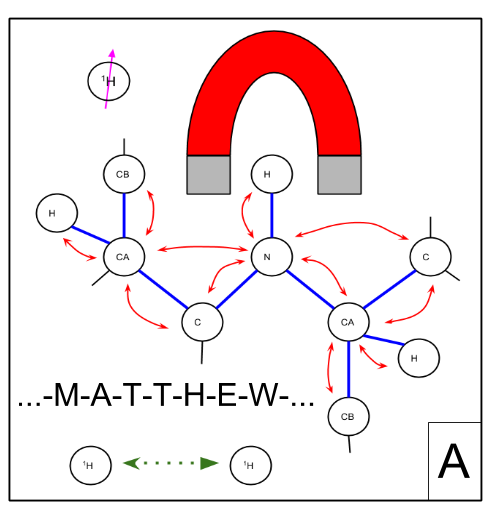
\includegraphics[scale=0.7]{figures/data_overview_1}
  \caption[General NMR and molecular knowledge.]
          {General NMR and molecular knowledge, including NMR phenomenon
           such as through-bond and through-space interactions, primary
           sequence, and gyromagnetic ratios.}
  \label{data_overview_1}
\end{figure}

\begin{figure}
  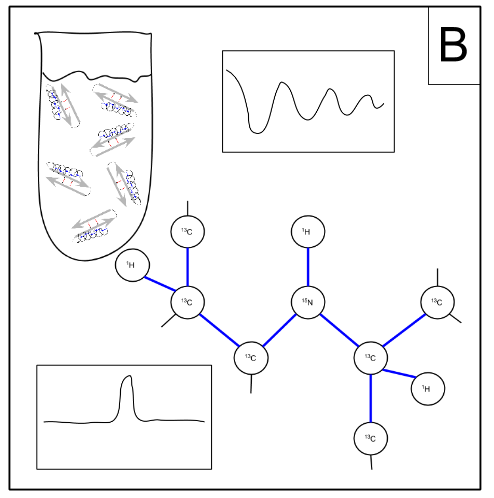
\includegraphics[scale=0.7]{figures/data_overview_2}
  \caption[Experimentally determined knowledge: obtained before analysis.]
          {Experimentally determined knowledge: obtained before analysis,
           including sample preparation and conditions, isotopic labeling,
           and time-domain and frequency-domain data.}
  \label{data_overview_2}
\end{figure}

\begin{figure}
  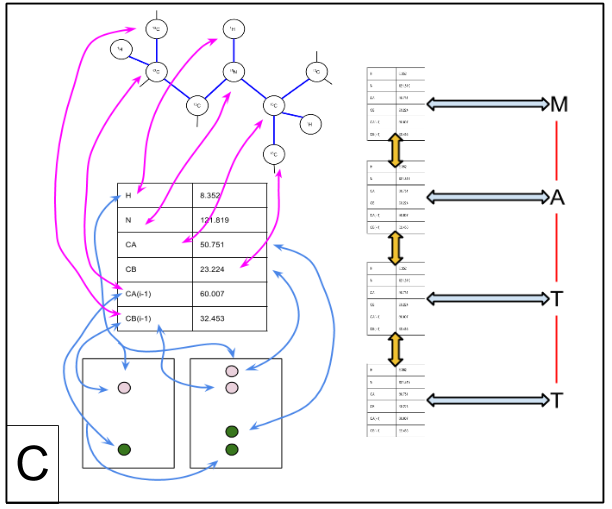
\includegraphics[scale=0.6]{figures/data_overview_3}
  \caption[Knowledge obtained during analysis.]
          {Knowledge obtained during analysis, including peaks, GSSs,
           resonances, sequential and sequence-specific assignments, and
           chemical shifts.}
  \label{data_overview_3}
\end{figure}

\begin{figure}
  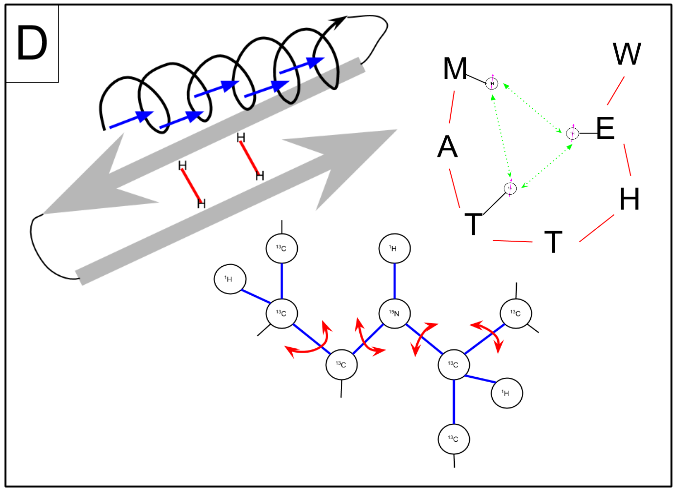
\includegraphics[scale=0.6]{figures/data_overview_4}
  \caption[Information about the actual physical properties of a molecule.]
          {Information about the actual physical properties of a molecule
           is derived from structural and angle restraints.}
  \label{data_overview_4}
\end{figure}

\begin{figure}
  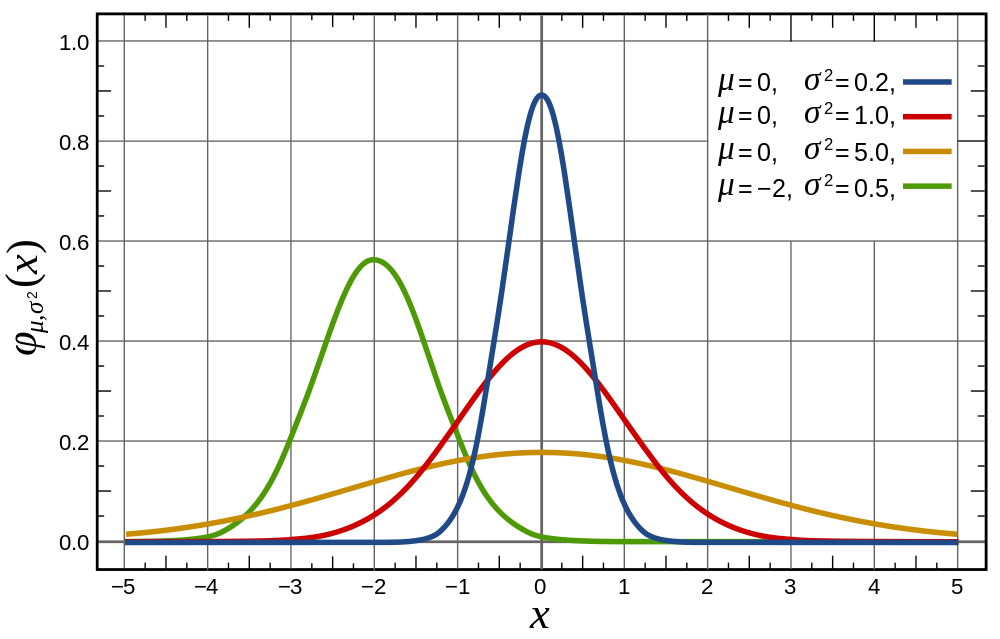
\includegraphics[scale=0.4]{figures/peak_1d}
  \caption[A 1-dimensional cross-section of Gaussian peaks.]
          {A 1-dimensional cross-section of Gaussian peaks.
           Each peak cross section may be characterized by its 
           position, as well as its width.  The peak as a whole
           has an intensity or height.  This image is in the
           public domain and was accessed at 
           \url{http://en.wikipedia.org/wiki/File:Normal_Distribution_PDF.svg}.}
  \label{peak_1d}
\end{figure}

\begin{figure}
  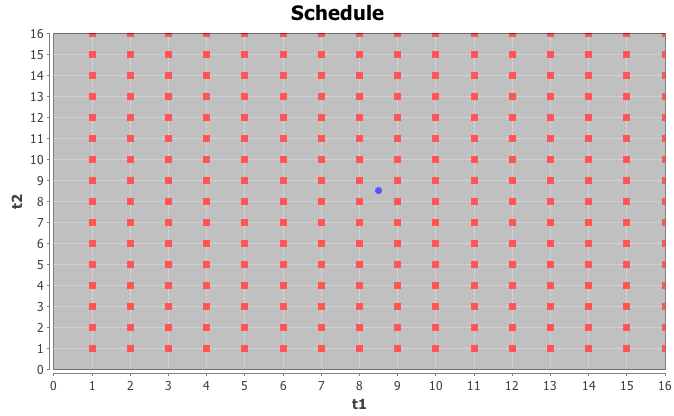
\includegraphics[scale=0.5]{figures/schedule_uniform}
  \caption[A uniform sample schedule.]
          {A uniform sample schedule.  The gaps between the points
           are constant.  The two axes represent the 
           variable time delays in the two indirect dimensions of a
           three-dimensional experiment.}
  \label{schedule_uniform}
\end{figure}

\begin{figure}
  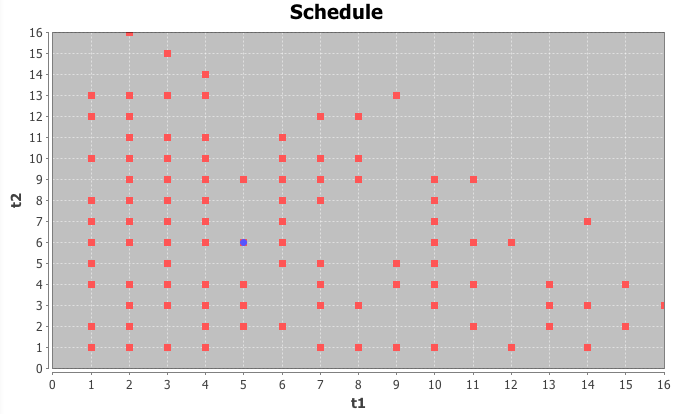
\includegraphics[scale=0.5]{figures/schedule_nonuniform}
  \caption[A non-uniform sample schedule.]
          {A non-uniform sample schedule.  The gaps between the points
           are not constant.  The two axes represent the 
           variable time delays in the two indirect dimensions of a
           three-dimensional experiment.}
  \label{schedule_nonuniform}
\end{figure}

\begin{figure}
  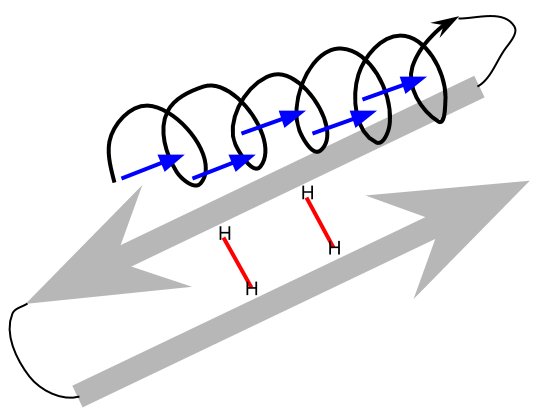
\includegraphics[scale=0.6]{figures/structure_restraints}
  \caption[Restraints are used to build a structural model.]
          {Restraints are used to build a structural model.
           Residual dipolar couplings give orientation constraints,
           and NOESY spectra give interatomic (H-H) distance constraints.}
  \label{structure_restraints}
\end{figure}

\begin{figure}
  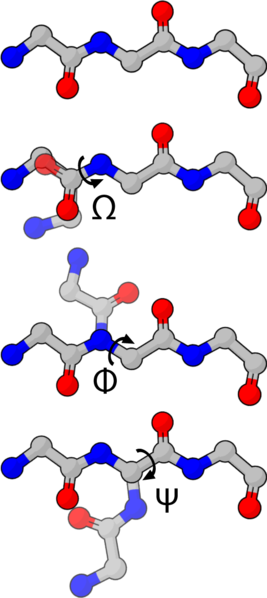
\includegraphics[scale=0.5]{figures/torsion_angles}
  \caption[Torsion angles provide structural information.]
          {Torsion angles provide structural information.
           A torsion angle is described by the positions of four
           atoms, and is the angle between two planes.  For protein
           structures, two key torsion angles are between the backbone
           atoms of each residue.
           This image is in the public domain, and was accessed
           from \url{http://en.wikipedia.org/wiki/File:Peptide_angles.png}.}
  \label{torsion_angles}
\end{figure}

% prevents a "! LaTeX Error: Too many unprocessed floats."
% see http://tex.stackexchange.com/a/46514/28358
\clearpage

\begin{figure}
  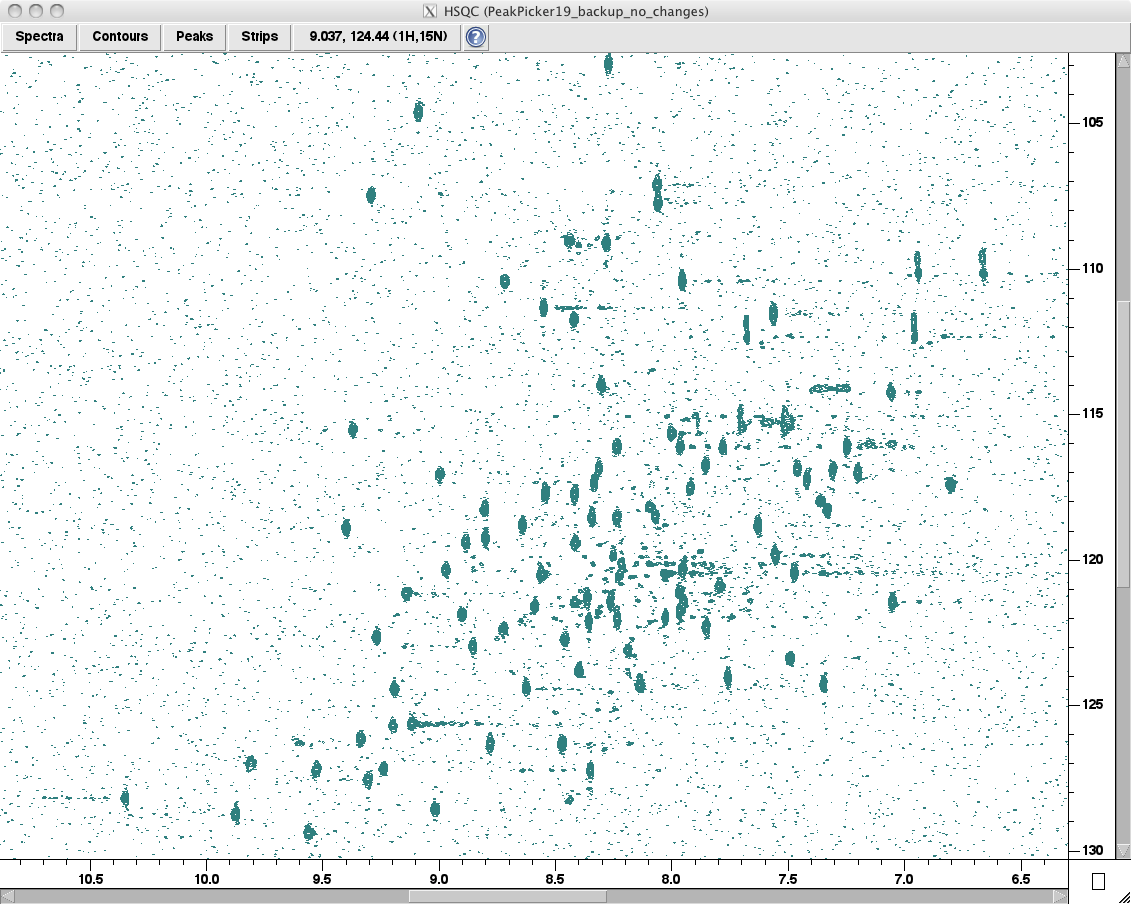
\includegraphics[scale=0.35]{figures/nhsqc}
  \caption[A frequency-domain NHSQC spectrum.]
          {A frequency-domain NHSQC spectrum. 
           The x- and y-axes are nitrogen and proton, respectively.}
  \label{nhsqc}
\end{figure}

\begin{figure}
  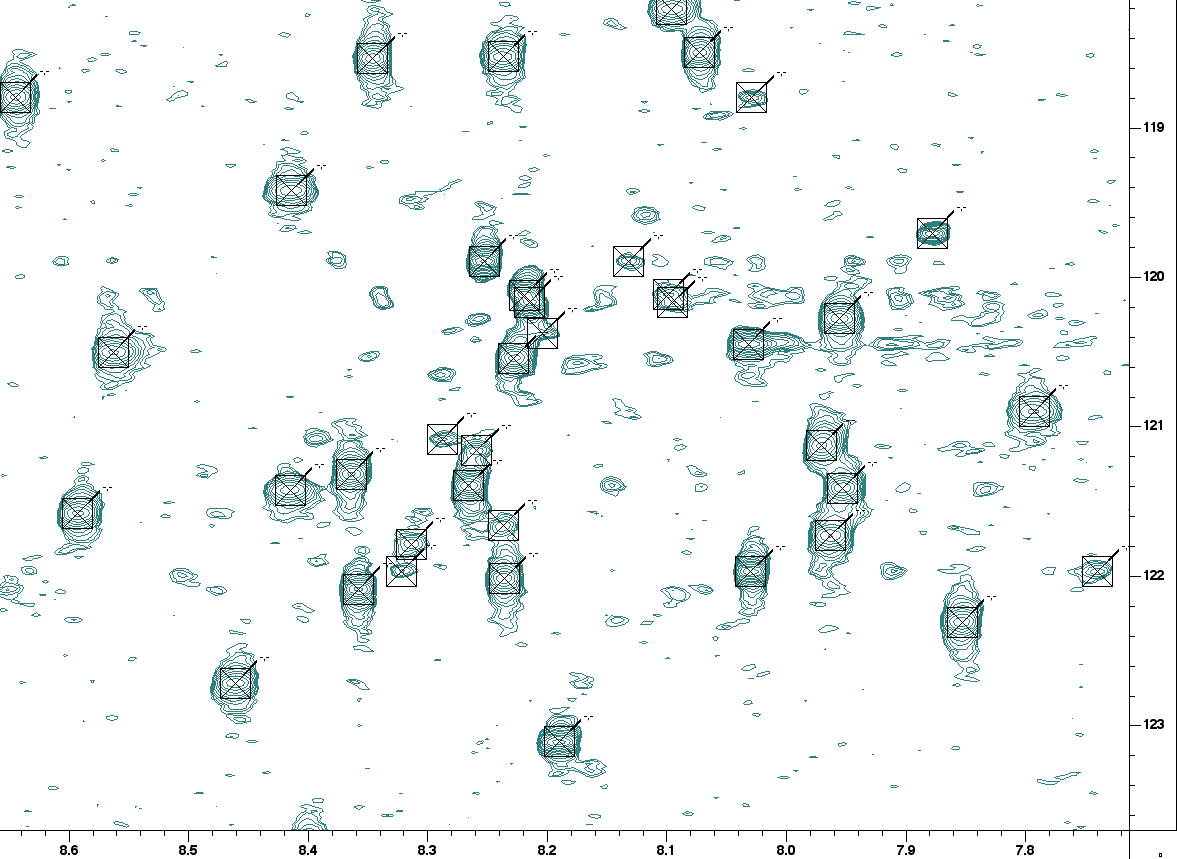
\includegraphics[scale=0.35]{figures/nhsqc_peaks}
  \caption[A peak picked NHSQC spectrum.]
          {A peak picked NHSQC spectrum. 
           Peaks are indicated by squares and crosses.}
  \label{nhsqc_peaks}
\end{figure}

\begin{figure}
  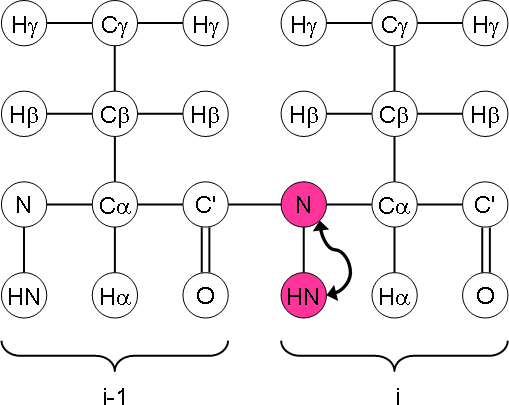
\includegraphics[scale=0.75]{figures/ccpn_nhsqc}
  \caption[The nuclei correlated by an NHSQC.]
          {The nuclei correlated by an NHSQC.
           This figure is reproduced from \url{http://www.protein-nmr.org.uk/}
           with the permission of Victoria Higman.}
  \label{ccpn_nhsqc}
\end{figure}

\begin{figure}
  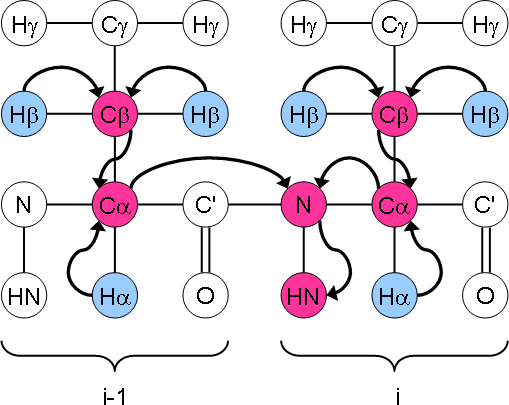
\includegraphics[scale=0.75]{figures/ccpn_hncacb}
  \caption[The nuclei correlated by an HNCACB.]
          {The nuclei correlated by an HNCACB.
           This figure is reproduced from \url{http://www.protein-nmr.org.uk/}
           with the permission of Victoria Higman.}
  \label{ccpn_hncacb}
\end{figure}

\begin{figure}
  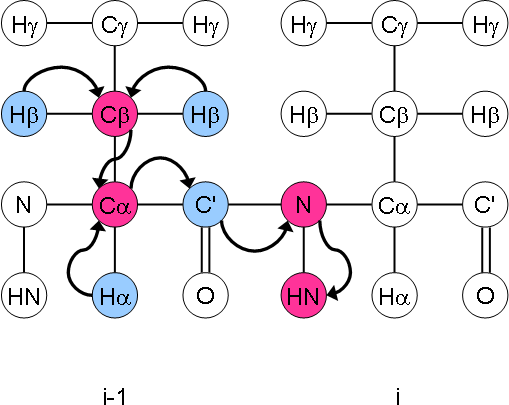
\includegraphics[scale=0.75]{figures/ccpn_cbcaconh}
  \caption[The nuclei correlated by a CBCA(CO)NH.]
          {The nuclei correlated by a CBCA(CO)NH.
           This figure is reproduced from \url{http://www.protein-nmr.org.uk/}
           with the permission of Victoria Higman.}
  \label{ccpn_cbcaconh}
\end{figure}

\begin{figure}
  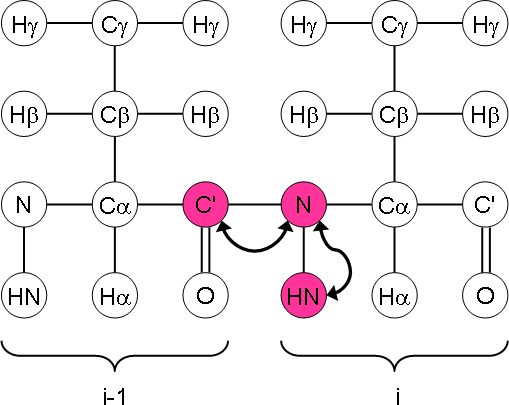
\includegraphics[scale=0.75]{figures/ccpn_hnco}
  \caption[The nuclei correlated by an HNCO.]
          {The nuclei correlated by an HNCO.
           This figure is reproduced from \url{http://www.protein-nmr.org.uk/}
           with the permission of Victoria Higman.}
  \label{ccpn_hnco}
\end{figure}

\begin{figure}
  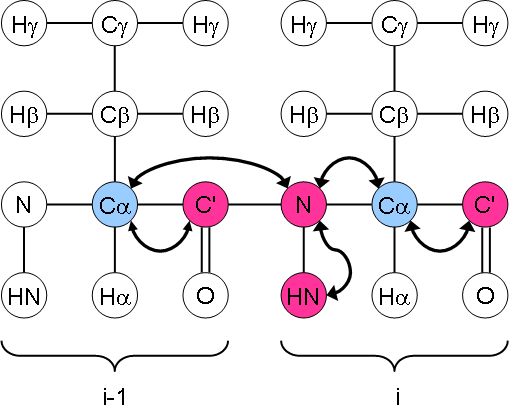
\includegraphics[scale=0.75]{figures/ccpn_hncaco}
  \caption[The nuclei correlated by an HN(CA)CO.]
          {The nuclei correlated by an HN(CA)CO.
           This figure is reproduced from \url{http://www.protein-nmr.org.uk/}
           with the permission of Victoria Higman.}
  \label{ccpn_hncaco}
\end{figure}

\begin{figure}
  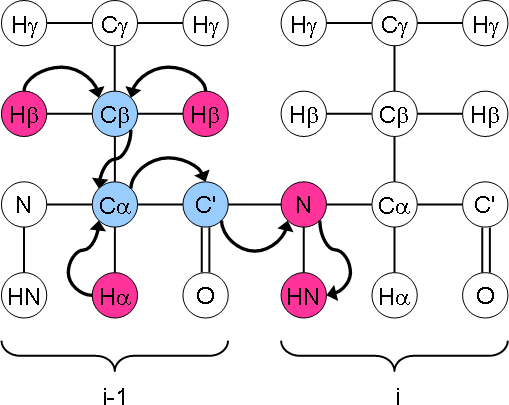
\includegraphics[scale=0.75]{figures/ccpn_hbhaconh}
  \caption[The nuclei correlated by an HBHA(CO)NH.]
          {The nuclei correlated by an HBHA(CO)NH.
           This figure is reproduced from \url{http://www.protein-nmr.org.uk/}
           with the permission of Victoria Higman.}
  \label{ccpn_hbhaconh}
\end{figure}

\begin{figure}
  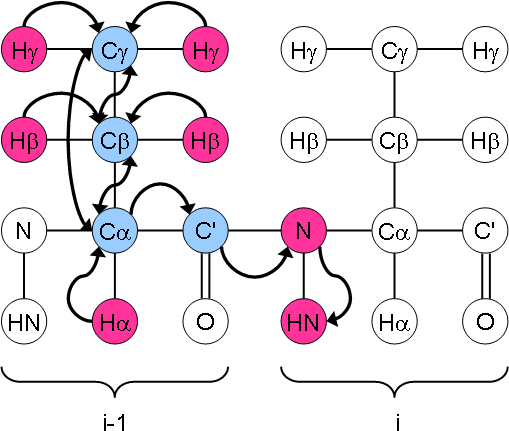
\includegraphics[scale=0.75]{figures/ccpn_hcconhtocsy}
  \caption[The nuclei correlated by an H(CCO)NH-TOCSY.]
          {The nuclei correlated by an H(CCO)NH-TOCSY.
           This figure is reproduced from \url{http://www.protein-nmr.org.uk/}
           with the permission of Victoria Higman.}
  \label{ccpn_hcconhtocsy}
\end{figure}

\begin{figure}
  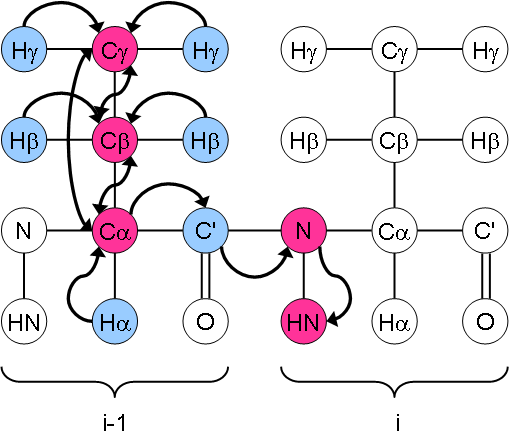
\includegraphics[scale=0.75]{figures/ccpn_cconhtocsy}
  \caption[The nuclei correlated by a C(CO)NH-TOCSY.]
          {The nuclei correlated by a C(CO)NH-TOCSY.
           This figure is reproduced from \url{http://www.protein-nmr.org.uk/}
           with the permission of Victoria Higman.}
  \label{ccpn_cconhtocsy}
\end{figure}

\begin{figure}
  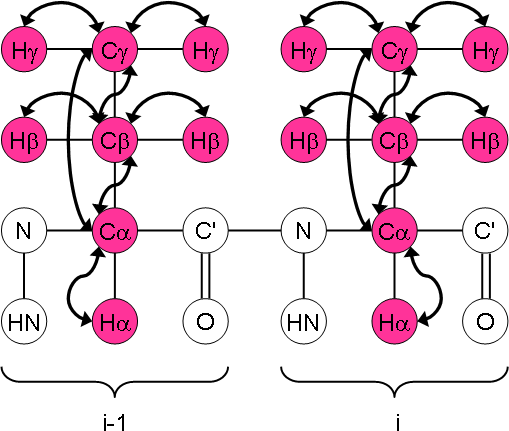
\includegraphics[scale=0.75]{figures/ccpn_hcchtocsy}
  \caption[The nuclei correlated by an HCCH-TOCSY.]
          {The nuclei correlated by an HCCH-TOCSY.
           This figure is reproduced from \url{http://www.protein-nmr.org.uk/}
           with the permission of Victoria Higman.}
  \label{ccpn_hcchtocsy}
\end{figure}



\chapter{A Process Overview}

\begin{center}
  \textit{If you can't describe what you are doing as a process, you don't 
          know what you're doing.}

 - W. Edwards Deming
\end{center}

This chapter will describe the NMR data analysis process in detail,
including the roles of computational and manual analysis, their interaction
with the data types, and tools used in the process.
In order to study proteins in solution using NMR, a multi-step process is 
employed to collect and analyze data, as shown in 
Figure \ref{nmr_overview}, which breaks the process down into a series of 
independent stages \cite{guerry2011automated}.
Figure \ref{process_timeline} shows a view of the process in the context
of the data discussed in the previous chapter.



\section{Data Collection}

See panel A of Figure \ref{nmr_overview}.

\subsection*{Sample preparation}
The protein or molecule of interest is isolated and a solution 
obtained.  The preparation procedure employed will determine isotope labeling
and concentration.

\subsection*{Time-domain data acquisition}
The solution is placed in an NMR spectrometer and an array of pulse sequences
are used to collect time-domain data.

The collection of data suitable for Fourier Transform processing, described
in the next section, requires uniformly collected data in each dimension.

Sensitivity, which determines the ability to discern true signals
from noise in the frequency domain, places constraints on data collection
\cite{rovnyak2004accelerated}.  Non-uniform sampling approaches 
\cite{maciejewski2011random} avoid these tradeoffs by collecting more data
points where the signal-to-noise ratio is high, but maintain resolution by
still collecting some data points where the signal-to-noise is low.


\section{Spectral processing}

In Figure \ref{nmr_overview} panel B, 
spectral processing operates on these FID data sets.  They are 
converted to frequency-domain spectra using tools such as NMRPipe \cite{nmrpipe}
and the Rowland NMR ToolKit \cite{rnmrtk}.  Functions such as 
zero-fills, Fourier transforms, phase shifts, apodizations, and linear 
predictions are applied to the data as a processing pipeline.  These 
functions are used to ensure that the spectra are amenable to further 
analysis, by optimizing peak size and shape and minimizing processing 
artifacts.

The raw data collected from an NMR spectrometer is referred to as 
time-domain data.  In a typical NMR experiment, these data represent the 
sum of multiple decaying sinusoids.  These FIDs are converted to 
frequency-domain spectra which are used in further analysis.  The goal of 
this phase is to construct a frequency spectrum which indicates the resonance 
frequencies of the nuclei that were observed in the experiment.  A common tool 
for such a transformation is the Fourier Transform, which is able to convert 
a uniformly collected data set into a frequency spectrum.  
An example of an NMR spectrum of N-H groups is shown in Figure \ref{nhsqc}.
Due to relaxation decreasing the amplitude of an NMR signal over time, peaks 
have an intrinsic linewidth in the frequency spectrum.
Related approaches include multidimensional decomposition \cite{mdd}
and maximum entropy reconstruction \cite{hoch1996nmr}.  When FIDs are 
non-uniformly collected, these processing methods are required.

Considerations include minimization of processing artifacts, signal-to-noise 
ratio, accounting for water lines, avoiding rolling baselines and baseline 
offsets, linewidth and shape, phasing, and apodization.  Multiple software 
packages exist for carrying out this conversion, such as NMRPipe and RNMRTK \cite{nmrpipe, rnmrtk}.
These packages include functions for processing the data in specific ways to 
guarantee desirable qualities.  A typical procedure for spectral processing 
involves the sequential application of multiple functions from one of these 
packages.  At each stage, the input is a data set and associated metadata, 
which includes information such as spectral width, dwell time, and number of 
points.  Each function may require the setting of one or more parameters in 
order to proceed.  Thus, in addition to the final frequency-domain spectrum, 
the process generates several intermediate data sets, several 
intermediate metadata sets, and the sequence of functions used along with 
their parameterizations.  A previous program developed by our lab, known
as CONNJUR WB, has enabled the convenient collection of necessary metadata 
during spectral processing \cite{connjur-wb}.



\section{Spectral analysis}

In the spectral analysis stage, Figure \ref{nmr_overview} panel C,
the overall goal is to identify the chemical shifts of individual nuclei.
The spectra may be analyzed using a tool such as XEasy \cite{xeasy}, 
Sparky \cite{sparky}, NMRViewJ \cite{nmrviewj}, or CCPN Analysis \cite{ccpn}.  

In each spectrum, peak-picking is performed, and true signal peaks must 
be identified and separated from peaks caused by noise and artifacts.  
Additionally, signal peaks caused by contaminants must be identified.  
Next, GSSs are identified and constructed \cite{ccpn}. 
The connectivity of resonances in a GSS is exploited 
in through-bond experiments.  GSSs then must be assigned 
connectivities to other GSSs through overlap of mutual resonances, 
amino acid types, and finally specific residues of the sample of interest. 
Resonances must also be assigned to specific nuclei \cite{ccpn}, 
with the final result being that specific nuclei in the sample of interest 
are assigned chemical shift values.  Currently, 100\% assignments are not 
achievable due to several factors such as data quality, ambiguity,
missing resonances, and metal ions \cite{guerry2011automated}.
Between 80\% and 95\% completion may be required \cite{williamson2009automated}
for successful analysis at later stages.

\subsection*{Peak picking}
Peak picking is the process of identifying and characterizing the peaks in 
a spectrum.  The goal is to identify all true signal peaks, while recognizing
and separating false peaks.

To a first approximation, a peak is identified by a local maximum in the 
frequency spectrum.  However, not all local maxima are necessarily true
peaks: noise and artifacts give rise to false peaks.  Nor do all peaks show 
up as local maxima if 
they are weak and close to the noise level, which causes them 
to be nearly indistinguishable from the noise and baseline; this may be due to 
sample instability such as aggregation or precipitation, or low sample 
concentration \cite{picky, munin, korzhnev2001munin, apart, autopsy, pine}
\cite{williamson2009automated, guntert2009automated, altieri2004automation,
baran2004automated}.
Each peak cross section has a non-zero width; adjacent signals may give rise
to overlapping peaks, distorting measurement of their attributes and possibly
also leading to disappearance of a local maximum.
Figure \ref{nhsqc_peaks} shows a portion of a peak-picked
NHSQC spectrum; note the overlap, and that some -- but not
all -- low-intensity spectral features have been identified as peaks.

Given these inherent issues, a general strategy for peak picking is 
described in \cite{autopsy, picky} and summarized here.
First, the noise level is estimated and points below the noise are discarded.
Next, of the remaining spectral regions, isolated areas are picked as peaks.
Finally, overlap is resolved by lineshape matching, the peaks are picked
and their attributes measured.  An optional additional step is filtering
based on symmetry and linewidth \cite{autopsy, picky}.

Correct peaks are important because they form the basis for the construction 
of GSSs, the assignment of chemical shifts to nuclei, and the interpretation of 
NOESY spectra which give rise to distance restraints as a preliminary to 
structure calculation \cite{guerry2011automated}.  
Incorrect peak identification or position can result 
in misinterpretation of NOESY spectra, which could lead to false distance 
restraints between atoms which are in fact very far apart in the actual 
protein structure.

Estimates of the amount of false positive and false negative peaks picked 
by computational tools range from low (10-40\%) to high (70-135\%) \cite{pine}. 
The quality of the results generally depends on characteristics of the 
spectrum, especially the signal/noise ratio, and resolution, as well as 
characteristics of the molecule including \mattfttwo{} (which has an 
effect on peak width) and number of nuclei -- more nuclei give rise to
more peaks, and therefore a higher chance of overlap.

Since none of these approaches yields perfect 
results \cite{guerry2011automated}, manual intervention during peak picking 
is important for obtaining results of sufficiently high quality
\cite{guntert2009automated}; many peak picking 
programs allow and encourage semi-automated interaction in order to clear 
up troublesome spectral features.  
Manual intervention is often accomplished based on knowledge outside of the 
spectrum: existence, position, and shape of peaks in other spectra, knowledge 
of the solvent, characteristic artifactual patterns caused by a specific 
processing scheme, knowledge of the local dynamics of a small region of the 
protein.  \cite{williamson2009automated, guntert2009automated, 
altieri2004automation, baran2004automated}
Because of this, peak picking can often not be completely finished until 
later analysis has been accomplished.

\subsection*{GSS and resonance construction}
As many pulse sequences are specificially designed to exploit the strong
backbone H-N coupling and correlate additional nearby nuclei, H-N groups appear 
in many through-bond spectra and are given a privileged position in analysis: 
the signals which H-N groups give rise to appear at matching chemical shifts
across multiple spectra.
This H-N matching enables grouping of peaks into GSSs; given multiple spectra
which include N-H dimensions, peaks with matching N and H chemical shifts are
determined to belong to the same GSS.
Table \ref{pulse_sequences} shows that H-N chemical shifts are captured in 
multiple spectra, and sometimes multiple times within a single spectrum.
At a later stage, GSSs are often augmented with additional sidechain resonances.
	
In addition to GSSs of backbone resonances, H-N-rooted GSSs typically are 
visible for Asparagine and Glutamine sidechains, and smaller GSSs of 
Tryptophan sidechains are visible.  Arginine sidechains may also give rise 
to an H-N-rooted GSS under certain experimental conditions. 

The difficulty in constructing these GSSs correctly and unambiguously stems 
from the issues inherent in NMR data.  First, the success of the standard 
suite of experiments rooted in H-N -- NHSQC, HNCO, HNCACB, etc. -- depends 
on \cite{autoassign1997}: % page 600 -- `reliability`
\begin{enumerate}
  \item good dispersion, i.e. no overlap, otherwise it is difficult to determine 
    which peaks belong with which H-N-rooted spin system.
  \item the H-N chemical shifts being nearly identical across all spectra.  
    This may not be the case if there are variations in the sample or the 
    temperature.  The Bloch-Siegert shift and experimental error also can have 
    an effect on chemical shift.
  \item nuclei appearing at a single chemical shift.  If there are multiple 
    conformations or chemical heterogeneity \cite{autoassign1997}, 
    a nucleus may appear at multiple chemical shifts and appear to be two 
    different resonances.
  \item the presence of an H-N group -- Proline is a notable exception, and 
    so it does not show up in experiments which rely on the presence of an H-N group
  \item extraneous peaks which do not seem to fit into a spin system, or 
    peaks which do not seem to match peaks in other spectra
  \item accurate (or at least consistent) spectral referencing.  
    Misreferenced spectra will cause the same nucleus to show up at different 
    chemical shifts across multiple spectra.
  \item quality of peak-picking \cite{autoassign1997, mars}: 
    chemical shifts, lineshapes, as well as the numbers of 
    false positives, false negatives, extraneous peaks
\end{enumerate}

Computational approaches for GSS construction tend to require manual 
assistance in some cases, such as AutoAssign and Mars 
\cite{autoassign1997, mars}.  Incorrect or 
incomplete GSSs will have negative effects on the quality of later 
analysis; several assignment tools assume that manual intervention will 
verify and, if necessary, correct the GSSs \cite{williamson2009automated}; 
this allows the tools to be conservative in their 
predictions \cite{autoassign1997}.  However, it may not be 
possible to unambiguously and completely construct GSSs until the results 
of later analysis are available: some approaches use NOESY peaks and 
assignments as well as structure results to verify and correct GSSs 
\cite{autoassign1997}.

Figure \ref{nhsqc_hncacb} shows an example of matching peaks between two
spectra.  The quality of the match -- how closely the chemical shifts line up,
as well as the lack of overlapping peaks -- means the peaks are easily
identified as members of the same GSS.

\subsection*{Resonance typing}
Before assigning a resonance to a specific 
nuclei, the type of a resonance may be assigned.  In an HNCO experiment, 
this is typically straightforward, because for each backbone spin system, 
the H dimension always corresponds to the backbone H, the N dimension always 
corresponds to the backbone N, and the C dimension always corresponds to the 
backbone C(i-1).  However, the situation is more complicated in an HNCACB 
experiment, as there are generally four choices of type assignment for 
the C dimension:  CA, CB, CA(i-1), and CB(i-1).  Thus, the resonance given 
by the C dimension of each peak must be assigned one of these choices.  
Reasons for choosing a specific assignment include peak sign, as well as 
chemical shift compared to statistics available in the BMRB.  In addition, 
the overlap between experiment pairs such as the HNCACB and CBCA(CO)NH 
facilitates resonance typing: while the CA(i-1) and CB(i-1) 
are expected to appear in both experiments at the same chemical shift for 
a given backbone H-N root, the CA and CB are expected to appear only in the 
HNCACB spectrum.

\subsection*{GSS typing}
Correspondingly, GSSs are also assigned amino acid types.  This phase 
interacts strongly with the assignment of nuclei to resonances, in 
that the possible nuclei to which a resonance may be assigned depends 
on the amino acid type, and the expected chemical shift ranges for various 
types depends on amino acid type as well.  For instance, GSSs assigned 
to the Glycine amino acid type should not have a CB; and the CB resonance's 
chemical shift of a GSS assigned to Alanine is expected to be very different 
from all other CB chemical shifts.  Backbone amino acid types may be split 
into several categories \cite{saga} based on BMRB statistics for 
CA and CB chemical shifts \cite{bmrb}:
\begin{enumerate}
  \item Ala
  \item Gly 
  \item Pro
  \item Ser, Thr
  \item Val, Met, Lys, His, Arg, Glu, Gln, Trp, Cys
  \item Asp, Asn, Ile, Leu, Phe, Tyr
\end{enumerate}
However, GSS typings are complicated by several factors.  First, GSS typing 
requires correct and complete GSS construction.  Second, correctly assembled 
GSSs may include overlapped or extraneous peaks, expected peaks (based on a 
spectrum's typical results) may also be missing.  Third, most GSSs can not 
be uniquely typed based solely on CA and CB chemical shifts, as groups 5 and 
6 (above) as well as 4 are ambiguous.  Fourth, sidechain GSSs must be 
identified and separated.

\subsection*{Sequential GSS assignment}
Sequential GSS assignments exploit the previously mentioned overlap of pulse
sequences such as the HNCACB and HN(CA)CO.  Sequential GSSs 
are expected to have CA/CA(i-1), CB/CB(i-1), and CO/CO(i-1) resonances at 
identical chemical shifts.  This duplication enables sequential assignment 
of GSSs.  Note that there is substantial interaction between nucleus-resonance 
assignment and sequential GSS assignment: assigning two GSSs sequentially 
implies the CB vs CB(i-1), CA vs CA(i-1), and C vs C(i-1) type assignments 
of the resonances in both GSSs; knowing the resonance typings of 
two spin systems can prevent their sequential assignment (if, for example, the 
matching resonances are both CB(i-1)); and not knowing the resonance typing 
implies that the sequential GSS assignment may be invalid.  
Sequential GSS assignment is complicated by: 
\begin{enumerate}
  \item missing peaks, possibly caused 
  by local dynamics, which reduce the number of overlapping resonances between 
  potential sequential GSSs, and can also disrupt resonance typing 
  \item extraneous peaks, which may be false positives or caused by 
  multiple conformations of the protein, causing incorrect matches
  \item degeneracy of chemical shifts:  given two GSSs with identical CA(i-1) 
  and CB(i-1) resonances, as well as a third GSS with matching CA and CB 
  resonances, it is impossible to unambiguously assign sequentially solely 
  on the basis of chemical shift matching between the two GSSs 
  \cite{autoassign1997}.
\end{enumerate}

An example of GSS overlap is shown in Figure \ref{hncacb_overlap}.  Green peaks
are CA, and purple peaks are CB; note that one each of green and purple peaks
match between the two GSSs.

\subsection*{Sequence-specific GSS assignment}
Since backbone GSSs are H-N-rooted, a GSS is assigned to a 
backbone-amide; this implies the assignment of resonances to nuclei as well, 
based on matching of resonance typing.  When a typical GSS is assigned to a residue, 
the H, N, C, C(i-1), CA, CA(i-1), CB, and CB(i-1) nuclei will be assigned 
resonances as well.  Sequence-specific assignment interacts heavily with 
sequential GSS assignment, because the protein sequence must be compatible 
with the GSS sequence, where `compatible' means that the amino acid types 
of the GSS match those of the protein sequence.  Note that full assignment 
of amino acid type to GSS is not a prerequisite for GSS-residue assignment; 
in fact, GSS-residue assignment may lead to GSS-amino acid type assignment 
for sequentially connected GSSs.  GSS-residue assignment is facilitated by 
long chains of sequential GSSs in which some of the GSSs are typed as Serine, 
Threonine, Glycine, or Alanine.  The longer a GSS chain, the fewer places it 
might possibly fit into the protein sequence \cite{saga}.  Also, 
as sequence-specific assignment proceeds, the number of unassigned GSSs and 
residues decreases; the result is that initially ambiguous assignments become 
unambiguous as choices are removed.  Conversely, complications arise from 
incomplete sequential GSS assignments resulting in short, ambiguous chains.  
The presence of prolines generally ends chains due to the lack of a backbone 
H-N group.  Missing GSSs also terminate chains.  Relatively few Ser, Thr, Gly, 
and Ala residues means the number of unambiguous anchor points will be lower.

Figure \ref{ss-residue} shows an example of sequence-specific GSS assignment.
Although not all of the GSSs have been typed, the presence of a Glycine and
Serine in the GSS chain reduces the possible assignments to residues.
Additionally, the length of the GSS chain helps reduce the ambiguity compared
to shorter GSS chains.

\subsection*{Sidechain: spin system and resonance assignment}
The next group of experiments collects chemical shifts of sidechain atomic nuclei.  
These experiments include 
the HBHA(CO)NH \cite{hbhaconh} in Figure \ref{ccpn_hbhaconh}, 
the C(CO)NH-Tocsy \cite{cconhtocsy} in Figure \ref{ccpn_cconhtocsy}, 
the HC(CO)NH-Tocsy \cite{hcconhtocsy} in Figure \ref{ccpn_hcconhtocsy}, 
and the HCCH-Tocsy \cite{hcchtocsy} in Figure \ref{ccpn_hcchtocsy}.  
The purpose of these experiments is to 
obtain the chemical shift values of sidechain resonances of protons, since 
proton frequencies are necessary in order to interpret NOESY spectra.  To 
interpret these spectra, the peaks must be assigned to GSSs and the new 
resonances typed.  While several of these experiments 
are also rooted in backbone H-N groups, facilitating the addition of peaks 
to the correct GSS, others -- such as the HCCH-Tocsy -- are not.  These are 
analyzed by the matching of resonance chemical shifts with those from other 
experiments targeting sidechains.  Resonance typing can generally 
be made with reference to compiled BMRB statistics.  Complications in this 
phase include: stereospecificity -- nuclei such as HA2 and HA3 may give rise 
to different chemical shifts, but resolving the correspondence may be 
impossible without further data; overlap -- especially in the HCCH-Tocsy 
where sidechains of the same amino acid type but different residue may have 
many closing matching chemical shifts; overlap between resonances within the 
same GSS, especially in Leu and Ile; missing and extraneous data; and the 
difficulty of both obtaining and unambiguously interpreting aromatic data.  
New approaches for sidechain data collection and assignment have recently 
been developed \cite{mobli2010non, hiller2008apsy} which seek to address 
these issues by reducing ambiguity of chemical shifts.

\subsection*{Alternative approach: probabilistic assignment}
The previously described approach views analysis as a pipeline: input is 
transformed into output, which becomes the input for the next stage, and so on.  
PINE \cite{pine} removes the pipeline constraint by connecting each stage to 
each other and allowing information to flow freely; this enables statistical 
weighting of interpretation as well as dependencies such as peak picking 
on GSS construction (a dependency which is not possible in the pipeline 
approach).  PINE does not remove the need for manual intervention; it is
still assumed that some level of intervention is necessary to obtain the
best results \cite{pine}.


\section{Structure determination}

In the final stage, Figure \ref{nmr_overview} panel D, the chemical shift 
assignments are used to interpret the NOESY experiments and a structure
is calculated and refined.

\subsection*{NOESY peak-picking and assignment}
NOESY peaks provide structural restraints if it can be 
determined which protons gave rise to the peak.  Analysis of NOESY spectra 
therefore requires chemical shift assignments of nuclei to 
determine the protons involved in a peak.  
NOESY spectra are  processed and peak-picked, similarly to through-bond 
spectra, and resonance assignments of peaks made.  
Considerations used to analyze 
NOESY spectra include: symmetry -- a peak is expected to correspond to a 
matching peak with the frequencies of the two 1H dimensions swapped; patterns 
based on known proximity of nuclei from the primary sequence giving rise to 
many short-distance NOE peaks; and network anchoring.  Complications include 
overlap caused by degenerate chemical shifts of protons, leading to 
ambiguous interpretations of peak assignments; this can be greatly mitigated 
by the use of an extra dimension:  15N- or 13C-edited NOESY spectra reduce 
the ambiguity, as well as incorrect or incomplete chemical shift assignments.

NOESY assignment may be done automatically by programs such as CYANA and 
ARIA \cite{cyana2004, aria2003}.  
NOESY peak-picking may be automated as well by programs such as
MUNIN \cite{munin, korzhnev2001munin}.

An alternative approach is taken by ABACUS \cite{abacus_assignment}, which uses
Monte Carlo probabilistic methods for assignment, NOE assignment, and structure
calculation.  A key difference of the ABACUS approach is the reduced dependency
on the quality and analysis of through-bond experiments; through-bond experiments
are used mainly to assemble peaks into GSSs, but sequential connectivities are
obtained from NOESY experiments.  A more detailed explanation may be found at 
\url{http://www.nmr2.buffalo.edu/nesg.wiki/Resonance_Assignment/Abacus/Introduction_to_ABACUS}.
Importantly, input to ABACUS -- correct NOESY peak picking and GSS construction
-- must be complete and accurate.

\subsection*{Structure calculation}
The resonance assignments of the NOESY data are 
interpreted to obtain distance restraints, which are then used to calculate 
coarse-grained three-dimensional structures.  The structures may then be 
refined and fine-tuned using a computational tool such as 
Assisted Model Building with Energy Refinement (AMBER) \cite{amber}.  
Unambiguous resonance assignment of NOESY data purely on the basis of chemical 
shift assignments may often be impossible or impractical, due to degenerate 
chemical shifts and to non-stereospecific assignments.  While these 
ambiguities can often be resolved through the collection of additional 
NMR data, the expense involved in doing so may often make it more practical 
to attempt to resolve the ambiguities through a structure determination 
program such as CYANA \cite{cyana2004}.

CYANA is able to calculate a three-dimensional structure from NOESY peaks, 
chemical shift assignments, and distance restraints \cite{cyana2004, aria2003} 
using an iterative approach to NOESY peak assignment and building structural 
models.  It also requires secondary structure information in the form of 
torsion angle restraints as input; as
chemical shift values are correlated to secondary structure, as described
by secondary chemical shift statistics \cite{spera1991empirical}, secondary 
structure can be calculated from chemical shift assignments using a program 
such as TALOS+ \cite{talos+}.  As of version 3.0, CYANA is able to make use
of RDCs during structure calculation as well.

Chemical shift assignments may also be used to calculate potential structures.
CS-ROSETTA \cite{cs-rosetta} uses chemical shift assignments of nuclei in 
backbone GSSs and produces a set of structures.  The general method is to 
compare the chemical shifts with those of proteins of known chemical shift
and structure, and then to select structure fragments from those known 
proteins.  By assembling these fragments into a complete structure, a full
model is constructed.  Although CS-ROSETTA is computationally intensive, it
still offers a massive potential time savings by eliminating the need to
collect and analyse NOESY spectra.

Additional programs may be used to build, manipulate, and refine structures.
AMBER \cite{amber} is a set 
of force fields which facilitate simulation of molecular dynamics.  The
force fields are parameterizable and describe potential energy; when applied
to a molecule they provide a description of the molecule's potential energy. 
Major components of the force fields are contributed by atomic bonds, 
electron orbitals, bond torsions, van der Waals interactions, and electrostatics.
XPLOR-NIH \cite{xplor-nih} is a
powerful structural calculation and refinement program that is capable of
incorporating torsion angle restraints, j coupling restraints, isotope 
effects, 13C secondary shifts, proton chemical shift restraints, RDCS, and NOEs.
These data are modeled by means of a set of energy terms which the program
attempts to minimize.  XPLOR-NIH is also capable of modeling explicit 
solvent molecules in order to determine their effect on the structure, 
although this approach is superceded by the potential energy term model
to a certain extent \cite{xplor-nih}.



\section{Discussion}

The inherent NMR issues of ambiguous, missing, and extraneous data cause 
problems throughout the entire analysis process.  Correctly dealing with 
these issues is difficult, but absolutely critical in order to obtain 
high-quality results \cite{williamson2009automated, guntert2009automated, 
altieri2004automation, baran2004automated}.  As yet, computational tools 
are not able to deal perfectly with these issues, due to one or more of 
several basic limitations: 
\begin{enumerate}
  \item they require high-quality input in order to function correctly:
    SAGA \cite{saga}, ABACUS \cite{abacus_assignment}, Mars \cite{mars}, 
    AutoAssign \cite{autoassign2001}, EZ-ASSIGN \cite{ezassign},
    PINE \cite{pine}, and CYANA \cite{cyana2004};
  this input is generally assumed to have been manually prepared in order 
  to meet the stringent quality requirements of completeness and absence of 
  extraneous results
  \item even with high-quality input data, tools are not able to produce 
  perfect results 
  \item tools perform differently in different contexts, although 
  performance generally decreases as protein size increases and spectral quality 
  decreases
  \item manual verification and correction of the results is assumed, 
  even for tools that claim to be fully automated 
  \cite{williamson2009automated, guntert2009automated, altieri2004automation,
  baran2004automated}
\end{enumerate}

A key limitation of many analysis tools is the fixed input data.  While
this simplifies the use of the tool in a simple pipeline, it may also lead
to reduced quality of results and explain the necessity of manual intervention:  
while the input data that a tool handles is restricted, manual interventions can
make use of any additional information required to make specific deductions. 
Thus, PINE and related efforts  
are an exciting effort to loosen these incidental restrictions.  Initial 
results are promising, and show a marked improvement, although manual 
intervention is still assumed to be necessary in order to obtain the best 
results \cite{pine}.  Further tools such as SHIFTX2 and CHESHIRE 
\cite{shiftx2, cheshire}, which calculate chemical shifts from structure,  
bring additional information to bear, helping to validate assignments.
Table \ref{data_connections} and Figure \ref{process_timeline} show some
of the key connections between various data types, putting these tools in
the overall context of NMR data analysis.

Another exciting development is the rise of probabilistic methods 
\cite{saga, pine}.  These methods reflect the reality that the 
confidence of a specific interpretation depends on the exact state of the 
data; in other words, an assignment which is 50\% confident given only an 
HNCA spectrum may become 90\% confident if an HN(CO)CA spectrum is added.  
The significance of this confidence level is that it enables easy tracking 
of ambiguous and/or low-confidence interpretations -- i.e. those that stand 
to benefit from collecting additional data sets.  By including confidence 
values on all assignments, an understanding of the troublesome areas is 
facilitated.  This helps to reduce the cost of cascading errors -- if the 
uncertainty is tracked as a confidence level, further interpretations based 
on a highly uncertain datum will also receive low confidence levels.  In 
addition, confidence levels are an alternative to the inherent balance 
between completeness and correctness -- it is no longer necessary to 
sacrifice one for the other \cite{autoassign2001, pine}.


\section{Conclusions}

The massive amount of data involved in a structure determination process --
often on the order of gigabytes -- necessitates the use of computational
tools for data management as well as efficiency of analysis.  To address
specific problems in the NMR analysis process, many software implementations 
of useful data processing algorithms have been created, distributed, and 
maintained in recent years 
(\url{http://nmrbox.org/NMRbox.org/Registry.html}, 
\url{http://nmrwiki.org/wiki/index.php?title=Category:Software}, 
\url{http://bmrb.wisc.edu/tools/prog\_corner.shtml}).  
Additionally, several groups have 
accelerated the process by producing software tools spanning and integrating 
multiple steps to decrease the necessity for time-consuming human intervention
\cite{abacus_assignment}.
This allows automated or semi-automated structure determination for small 
proteins.  Other groups have built integrated pipelines, using one specific 
tool for each step \cite{baran2004automated, sail_flya}, 
and allowing manual intervention at traditionally 
difficult stages.  Many recent methods re-envision structure determination 
as an iterative process, where the results of a later stage may require the 
researcher to re-evaluate or re-perform an earlier stage \cite{cyana2004}; 
this has been applied to interpretation of NOE-derived 
restraints \cite{aria2003}.  Altogether, the structure determination 
process can often take several months \cite{guerry2011automated}.

In general, while computational tools are able to deliver results relatively 
quickly compared to manual analysis, they may not be able to produce more 
accurate results, especially when the input data is low-quality, irregular, or 
otherwise problematic; this can result in false positives and negatives
\cite{williamson2009automated}.  This is a problem at every stage of spectral
analysis.

This has the consequence that NMR structure determination data analysis 
processes cannot be fully automated if high-quality results are required.  
An effective solution to this problem combines the strengths of the automated 
and manual approaches, in a semi-automated fashion:  computational tools are 
used to quickly perform the majority of analyses such as peak-picking and 
GSS construction, and manual analysis is used to clear up the 
relatively small number of cases involving ambiguities and errors caused 
by problematic or unclear data.  Thus, some amount of manual analysis may 
be required at all stages of the data analysis process 
\cite{guntert2009automated, williamson2009automated}.   

Manual analysis therefore plays a critical role in NMR data analysis, due 
to the inherent issues of analysis which complicate automated tools, and 
to the ability to bring sufficient context to bear to solve difficult cases.  
Manual intervention is assumed to be necessary by 
most tools, even automated ones, to ensure the completeness and correctness 
of results.  However, despite the importance that manual intervention plays 
in analysis, the specific modifications made and their reasons for -- 
which may be quite complicated -- are not captured \cite{guntert2009automated}.  
Thus, the metadata of manual intervention is lost, and analysis is 
irreproducible.
Figure \ref{nmr_process} shows which data are and are not required for 
deposition by the BMRB, indicating data missing from final results that
prevents reproducibility.



% tables
\clearpage
\section{Tables}

% TODO more examples
% TODO some inputs, outputs have multiple data types
\begin{table}[h]
    \begin{tabular}{ | c || c | c | c | c | c |}
    \hline
      Data                                      &  Example              &  Reverse example   \\  \hline
      FID -> spectrum                           &  Frequency-domain     &  NMRPipe, RNMRTK   \\  \hline
      Spectrum -> peaks                         &  Sparky peak picker   &                    \\  \hline
      Peaks -> GSSs                             &                       &                    \\  \hline
      Sequence -> chemical shifts               &                       &  ShiftY            \\  \hline
      Chemical shifts -> secondary structure    &  TALOS+               &                    \\  \hline
      Chemical shifts -> tertiary structure     &  CS-ROSETTA, CHESHIRE &  SPARTA+, ShiftX   \\  \hline
      Chemical shifts -> NOESY assignments      &  CYANA                &                    \\  \hline
      NOESY assignments -> structure            &  CYANA                &                    \\  \hline
      NOEs, shifts, j-couplings -> structure    &  XPLOR-NIH            &                    \\  \hline
    \end{tabular}
    \caption{Connections between various data types.}
    \label{data_connections}
\end{table}



% figures
\clearpage
\section{Figures}

\begin{figure}[h]
  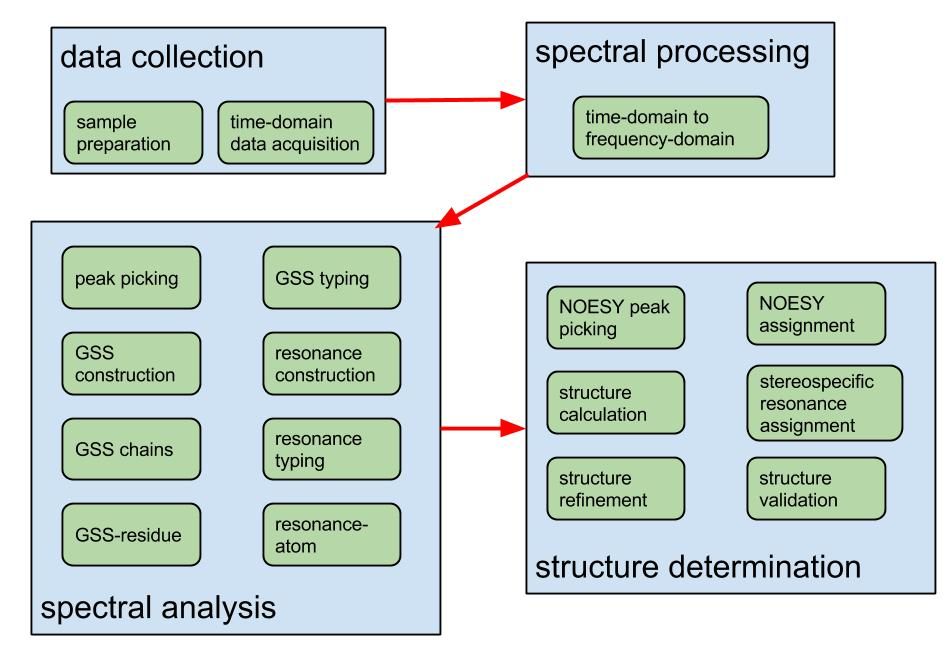
\includegraphics[scale=0.42]{figures/nmr_overview}
  \caption{An overview of the NMR process for protein structure determination}
  \label{nmr_overview}
\end{figure}

\begin{figure}
  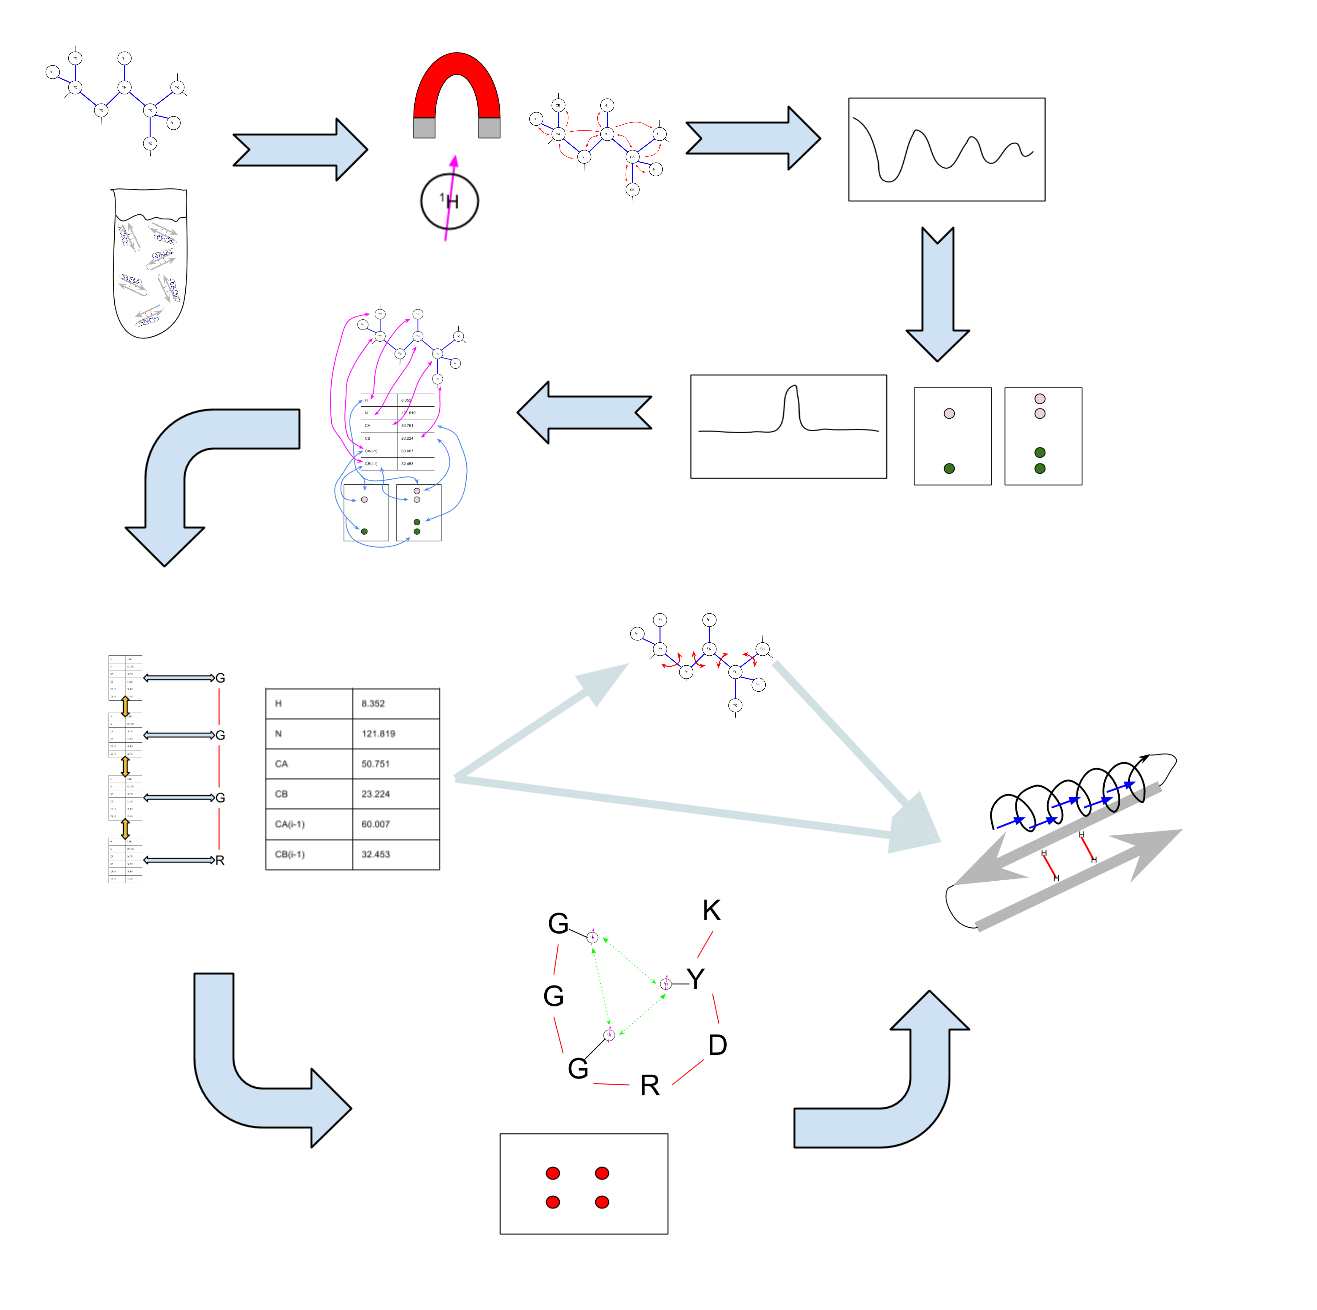
\includegraphics[scale=0.35]{figures/process_timeline}
  \caption{The connections between various data types.}
  \label{process_timeline}
\end{figure}

\begin{figure}
  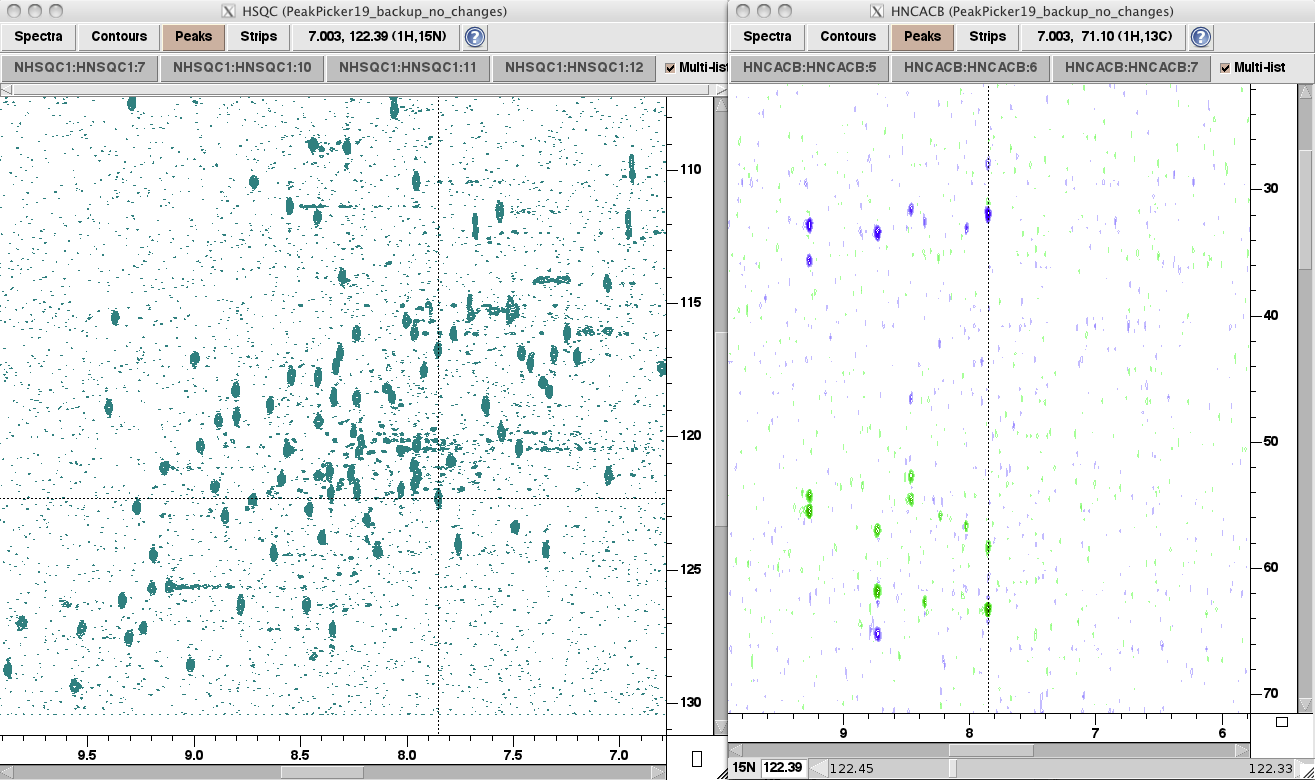
\includegraphics[scale=0.3]{figures/nhsqc_hncacb}
  \caption[Matching peaks between an NHSQC and an HNCACB spectrum]
          {Matching peaks between an NHSQC and an HNCACB spectrum.
           This likely indicates that the peaks belong to the same GSS.}
  \label{nhsqc_hncacb}
\end{figure}

\begin{figure}
  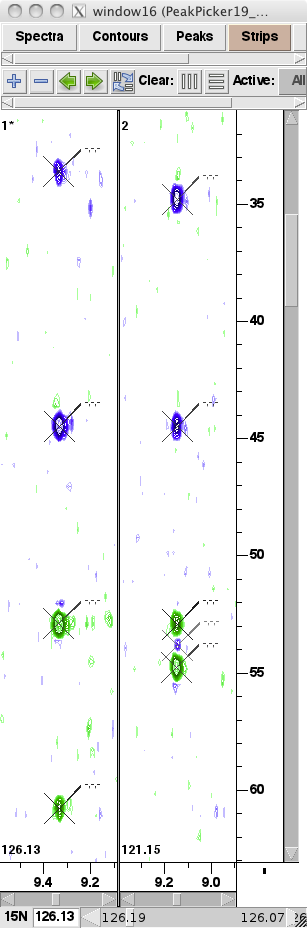
\includegraphics[scale=0.35]{figures/hncacb_overlap}
  \caption{Overlap of Carbon resonances in an HNCACB spectrum.}
  \label{hncacb_overlap}
\end{figure}

\begin{figure}
  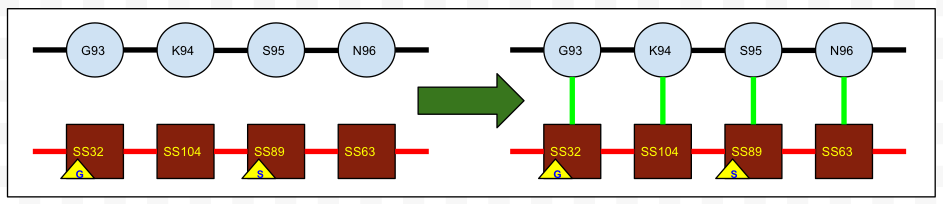
\includegraphics[scale=0.45]{figures/ss-residue}
  \caption[Assignment of a GSS chain to residues]
          {Assignment of a GSS chain to residues.  The circles are residues,
           black lines are peptide bonds, squares are GSSs, red lines are 
           sequential GSS assignments, and green lines are GSS-residue 
           assignments.}
  \label{ss-residue}
\end{figure}

\begin{figure}
  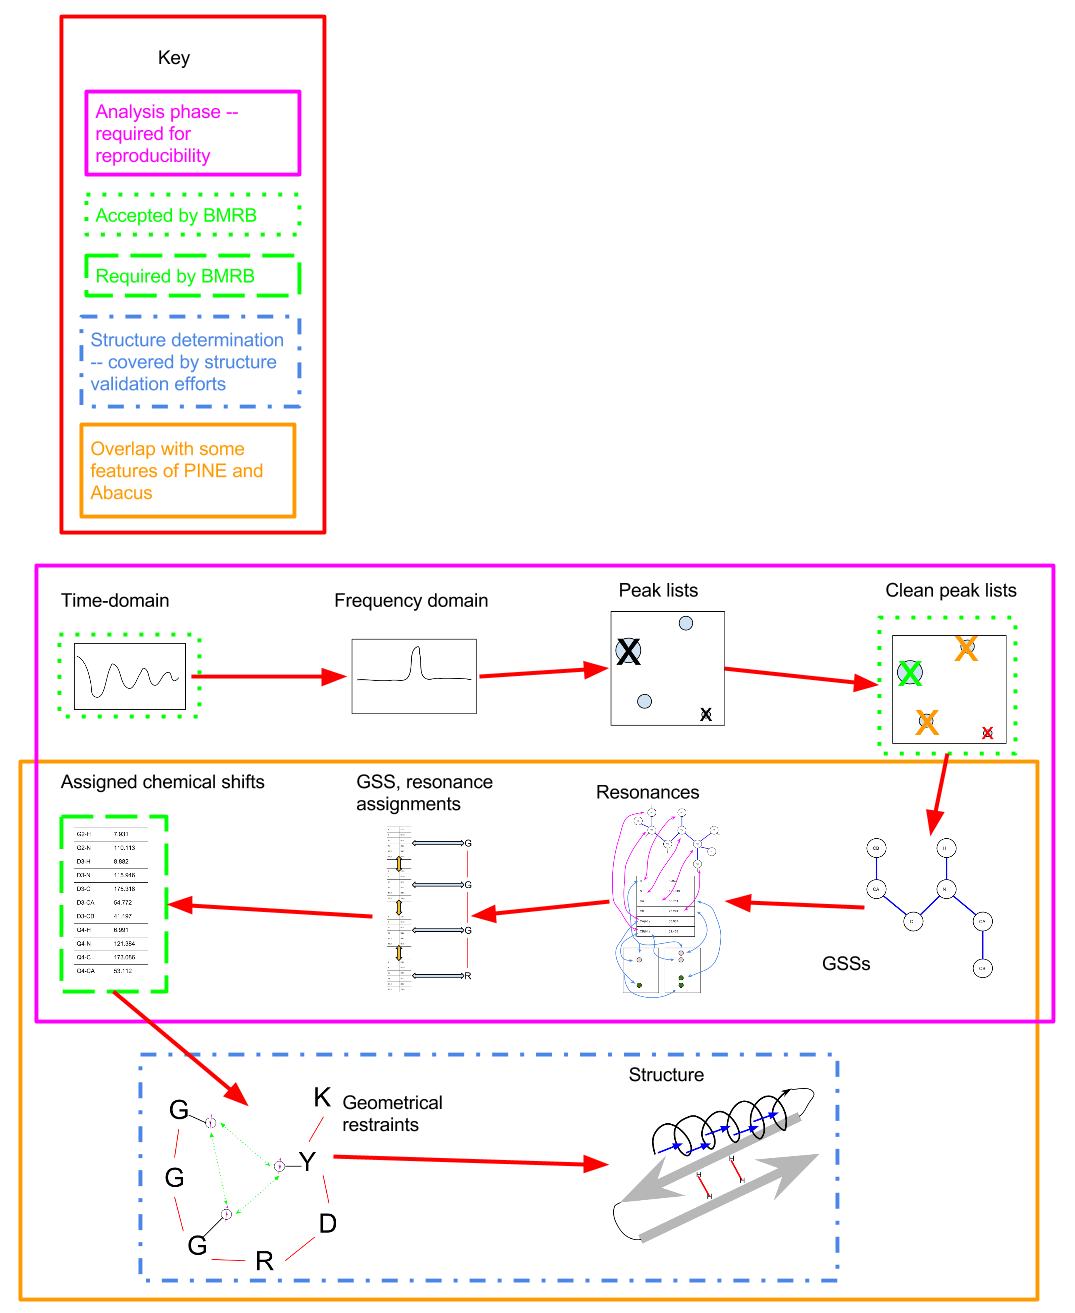
\includegraphics[scale=0.3]{figures/nmr_process}
  \caption[Breakdown of the NMR process by reproducibility.]
          {Breakdown of the NMR process by reproducibility.  The BMRB currently
           requires deposition of some data types, and accepts others.  However,
           these data are incomplete.}
  \label{nmr_process}
\end{figure}



\chapter{An Approach for Reproducible Analysis}

\begin{center}
  \textit{If you're doing an experiment, you should report everything that 
    you think might make it invalid - not only what you think is right about it; 
    other causes that could possibly explain your results; and things you 
    thought of that you've eliminated by some other experiment, and how they 
    worked - to make sure the other fellow can tell they have been eliminated.}

 - Richard Feynman
\end{center}



\section{NMR data analysis is irreproducible}
Successful achievement of a reproducible NMR study requires reproducibility at 
each stage of the process.  First, the protocol for expressing, purifying, and 
preparing the sample of interest for experiments inside the NMR spectrometer 
must be reproducible, as well as the exact experimental conditions, 
spectrometer, pulse sequences and collection times used to collect the 
time-domain data must be captured.  Second, the software, platform, functions, 
and parameterizations for spectral processing stage must be captured.  
Third, both the computational results of peak-picking, GSS construction,
GSS assignment, and resonance assignment as well as any manual changes, 
along with the associated deductive process of reasoning, must be captured.  
Fourth, analysis and assignment of NOESY spectra, structure calculation, 
stereospecific resonance assignment and structure refinement must be captured.  
This last stage may also include computational as well as manual analysis 
components.  

This work will focus on reproducibility of the third and fourth stages, 
spectral analysis and structure determination.  Unfortunately, according to 
the definition of reproducible NMR given above, these stages are irreproducible.

Much work has been done to capture additional data from the assignment process.  
The CCPNMR effort, including the significant projects of CCPN Analysis and the 
CCPN data model \cite{ccpn}, captures a significant portion of final data.
Other significant efforts include SPINS \cite{baran2006spins}, 
Sesame \cite{sesame}, and the NorthEast Structural Genomics consortium (NESG)
 \cite{nesg2005nmr}.  However, much of the previous 
work in this area has focused on project management rather than reproducibility.
While SPINS is effective at capturing intermediate and final results, it is 
only intended for use on primary data files -- it is not designed to capture 
the key meta data mentioned above.  Sesame is capable of project management; 
however, it is intended for use in high-throughput studies.  ELNs 
\cite{rubacha2011eln}, while effective at capturing experimental design and
data, are not designed to support in-depth analysis, nor are they intended
to interface with NMR tools.

While the need for integration of automation with occasional manual 
validation and editing has been recognized \cite{baran2006spins}, no 
current systems are capable of combining these features with full 
meta data capturing.  
What is still missing is an approach and tooling for collecting all the primary 
data and meta data of NMR spectral analysis and structure determination.  Much 
time and effort is expended in these stages, but the data is not recorded.  The 
result is that the final data sets deposited into the BMRB are incomplete.



NMR data analysis is irreproducible because insufficient information is
captured during the process.  
This chapter will outline the data involved in NMR, and then 
describe in more detail the missing data, its role and importance, 
then a model for capturing that data, and a strategy for using
the model during the analysis process.



\section{Concrete data sets}
The data involved in the NMR process was covered abstractly in Chapter 
\ref{ch_data_overview}.  During execution of the NMR process, these data
are embodied concretely as structured files, read to and written from
local hard drives, databases, and remote hosts.  Final data sets are 
deposited to the BMRB and are then shared as NMR-STAR files.  Since files
are used as the means of transfer and sharing of NMR information, it is 
necessary to define the meaning and extent of a data set in terms of the
number, format, and content of the data files involved.

In the data collection stage, the extent of a data set includes the FIDs
stored as structured binary files as well as the metadata describing
various parameters of how the data was recorded and saved.  The scope of
a data set is expanded during spectral reconstruction to include binary
spectral data, spectral metadata, and the sequence of functions used to
convert the data from time-domain to frequency-domain, which often takes
the form of a shell script file invoking processing tools.

During spectral analysis, a data set includes peak lists and chemical shift
assignments.  Depending on which analysis tool one uses, these data are saved
in various formats along with additional parameters and settings which 
describe the configuration and state of the tool itself (such as contour
levels and peak ornament colors on a spectral display) which are not of direct
importance to NMR.  When integrating analysis with tools such as TALOS+ and
CS-ROSETTA \cite{talos+, cs-rosetta}, specially formatted files may be 
temporarily generated to transmit information to those tools, such as 
chemical shift assignments in a specific format.  The protein sequence is
often stored as a textual file containing the protein's amino acids.

Once the structure determination stage is reached, the data set now includes
torsion angle restraints, structure files, lists of restraint violations, 
NOESY peak lists, RDC lists, and scripts for running and analyzing results 
from tools such as CYANA.



\section{Missing data and its role in analysis}
% need to cover what the data is, how it plays a role in NMR analysis, 
% why it's important to capture
The key deficiencies causing irreproducibility are missing primary data and 
meta data which are modeled neither in the CCPN data model nor in the 
NMR-STAR data dictionary, and are not archived and disseminated.
In other words, these data form an important piece of the analysis process,
but are not captured as concrete data in the data set.
Spectral analysis, including peak picking, GSS construction, GSS and resonance
typing, sequential GSS assignment, and sequence-specific GSS assignment is 
accomplished using a step-by-step process of deductive reasoning 
which is often augmented by computational tools.  The computational 
results may be subject to manual validation, correction, and extension
\cite{guerry2011automated}.  This section will explore the various types
of data involved.


\subsection*{Deductive process of reasoning}
Manual modifications are performed using a process similar to deductive 
reasoning.  It follows a general pattern:
\begin{enumerate}
  \item identification: a feature of the data is identified as amenable to 
    interpretation.  For example, the feature may be a false negative (such as 
    a signal peak misclassified as noise by the automated peak-picker), a false 
    positive (such as an artifactual peak misclassified as signal), or an 
    ambiguity (such as overlapped GSSs, causing clustering algorithms to fail).
  \item pattern recognition: the spectroscopist identifies a potential method 
    for interpreting the feature based on his/her domain knowledge of NMR and 
    experience with interpretation of previous data sets.  For example, such 
    methods may take the form of deductive rules:  if <the data matches a 
    certain pattern>, then <it could be interpreted a certain way>. 
  \item application of the rule to the data feature.  The chosen rule is 
    applied, and the result of the interpretation is included back into the 
    data set.  The result may now be used to drive further deductions.
  \item repeat -- go to step 1 to identify features for further interpretations
    This method is a form of iterative, sequential deduction.  The key components 
    are the ordered series of steps, the state of the data before and after each 
    step, and the deductive rules used to make interpretations at each step.  
    In addition, it should be noted that the final data set can not be 
    regenerated using automated tools alone if there are any manual 
    modifications made to tool output.
\end{enumerate}

The information describing the deductive process of reasoning employed in 
manually interpreting a feature of the primary data is not captured, although
it is important because it provides the explanation 
of why something was done.

Each deductive reason is an embodiment of NMR-specific knowledge of how to 
interpret a data feature.  In general, a deductive rule requires an input, 
produces an output, and has an intuitive justification for its action.
% TODO example

Application of these rules provides a rationale for manual modifications.  The
rationale is a justification that the change modification is correct, as
well as an indication of why the change was made.  Therefore, capturing the
deductive rules employed enables verification of the veracity of modifications. 
It also facilitates knowledge transfer, both in the contexts of collaboration
and teaching, by providing a meaningful annotation (with reference to the
domain of NMR) for actions taken.


\subsection*{Intermediate results: the data set is the deductive context}
When the output of a computational tool, whether peak-picking, GSS construction, 
or sequence-specific GSS assignment, is modified to correct mistakes,
a discrepancy is introduced between the output of the tool 
given the input and a suitable parameterization, and the final data set. 
This indicates that the final results are not the output of a single 
replicable step, but rather of a series of steps of refinement and 
modification.  Thus, new data sets are implicitly generated from the previous
one during the analysis process after every modification, whether manual or automated.
The application of a deductive rule to modify the data set is sensitive to
the current state of the data set -- in other words, the validity of the 
use of a given rule, as well as its effect, depends on the exact state of
the data set.  Therefore, it is important to record the data context when
applying a deductive rule.  The intermediate results rectifies the discrepancy 
between automated tool output and the final data set.  However, this data is 
not recorded.

With respect to reproducibility, the importance of capturing intermediates is 
due to the dependence of deductions on context: without knowing the context, 
it is impossible to evaluate the correctness, confidence, and alternative 
interpretations of a deduction.  In standard approaches to analysis, the 
contexts are not captured; they are implicit.  By making the contexts 
explicit, it becomes possible not only to fully recapitulate the process of 
analysis, but also to employ error detection and correction strategies by 
analysis of deductions and their contexts.  An interesting side-effect of 
capturing contexts is that analysis can be restarted in the middle, by 
selecting an appropriate context and applying a different deduction.

% TODO
% come up with a simple example that demonstrates: 
%   1) the dependence of deductive ability on context
%   2) the concept and utility of multiple snapshots
%   3) the concept and utility of tracking logical dependencies

Furthermore, during manual analysis and modification of results, when the 
state of the data is continually being modified and improved, the analyses
which may be made are dependent upon the data context.
For example, assignment of a GSS to a residue may allow a further 
unambiguous assignment of a different GSS to a residue (an assignment 
which previously would have been ambiguous) by eliminating one of two 
assignment possibilities based on matching amino acid type.
% TODO explain better, provide an example
Implicit in the sequence of data sets are logical dependencies of derived
data upon features of the previous data set: the context of each deduction
is important, because the exact context determines what deductions may be
made and the confidence level of each deduction. 

% TODO I need to discuss what the intermediate results need to do
%   i.e. they need to make the process recapitulatable
%   and this is done by capturing the contexts


\subsection*{Extraneous results}
Standard approaches use the 
assumption that all peaks are true signal, with no provision for storing peaks 
determined to be processing artifacts or noise.  Such spurious peaks are simply 
deleted and do not show up in the final results.  This is a problem because the 
fact that a peak was found, and later interpreted as noise does not show up in 
the final data set.  The same problem applies to GSSs that are found 
but can not be assigned to any residue of the sample of interest, or are 
believed to correspond to atomic nuclei of a contaminant.  Such GSSs should 
be represented in the final data set.

During analysis, some portion of the positive results are not of direct interest
to the final answer.  Not only peaks, but also resonances and GSSs are included.
The positive results include both false positives, caused by noise or
artifacts, and true positives, caused by contaminants.

Although not of direct interest, such extraneous results play a role in 
the process of analysis: as was covered earlier, when making a manual
modification, a deductive rule is applied to a context (data set).  Changing 
the context affects which rules apply and what deductions are made; 
therefore, as a part of the context, extraneous results matter during analysis. 
If incorrectly identified or left unrecognized, extraneous features can
lead to incorrect peak picking, chemical shift assignments, GSSs, and GSS
assignments.

A further benefit of capturing extraneous results is the ability to distinguish
between identifying a data feature and interpreting it.  In other words, peaks
picked during peak picking are treated as positives, this is the "identification"
phase; in the later "interpretation" phase, these peaks are separated into
false positives and true positives.  This allows rectification of the 
discrepancies between uncorrected computational results and the final,
deposited results as well as marking potentially suspicious results for 
future perusal.  It should also be noted that picking a peak, then
interpreting it as extraneous and discarding it is typically not reported in
final data sets, despite containing important information.
There is a balance between false positives and false negatives \cite{pine};
false negatives are more undesirable \cite{pine, saga, guntert2009automated},
and capturing extraneous results helps to avoid this tradeoff: by reducing
the cost of a false positive, tools are free to focus on avoiding false
negatives.

The process of separating positives into false and true is prone to 
introducing bias; by keeping and reporting the initial results, such bias
can be estimated.  This is not possible if the extraneous results are not
reported, and also allows the feature identification phase to proceed
without bias, since error correction will be applied at a later stage. 
By providing additional context, it may be possible to estimate the quality 
of an analysis, where errors may be most likely found in the borderline 
cases; it will also help assigning confidence levels to datums by not.
Additional quality measures enabled include the number of peaks found by the
peak-picker, the number of false positives, the number of peaks assigned to
GSSs, and the number of GSSs assigned to residues.  It may also be possible
to estimate contamination, incompleteness and overcompleteness, overfitting, 
and consistency.


\subsection*{Notes: incompletions, uncertainties, ambiguities}
During the course of data analysis, it is often the case that odd, ambiguous,
abnormal, or otherwise unexpected situations noticed during analysis
\cite{nuseibeh2000inconsistency}.  
% TODO however, no record is made, blah blah .... these are valuable b/c blah blah
As notes indicate the deficiencies and 
potential problems present in a data set, they are valuable to future 
scientists as they highlight a data set's flaws and how it can be improved.

Due to the difficulties inherent in data analysis, situations are reached
in which the interpretation of a specific feature is problematic:
\begin{itemize}
  \item uncertain or impossible.  The evidence for a particular deduction 
    is not solid.
  \item ambiguous.  Multiple interpretations of a feature are consistent
    with the data and satisfy the constraints.  It is not possible to choose
    between them.
  \item inconsistent.  The data set is in an inconsistent state, or a 
    deduction would leave it in an inconsistent state.
\end{itemize}
A simple example is non-stereospecific sidechain proton assignments: 
a residue such as a Histidine or Lysine which has two beta protons will 
often give rise to two resonances, one for each beta proton; however, 
without additional information, it is impossible to assign a resonance to
a specific nucleus.  A related example is caused by the two delta and epsilon
protons in Phenylalanine and Tyrosine aromatic sidechains; the two resonances,
even if distinguishable, can not be uniquely assigned to nuclei.  In both
cases, the ambiguity is resolvable through the use of additional information;
however, before that additional information is provided, it is useful to be
able to store what is known -- that there are two peaks, each of which 
corresonds to one nuclei, but exactly which is unsure -- as an indication to
future analysis or perusal that a problem has been identified but not yet
solved.

% TODO add a picture
Correctly identifying and characterizing peaks in the presence of significant
amounts of overlap is a notoriously difficult problem \cite{guerry2011automated}.
The number, position, and intensity of peaks become distorted by the overlap.
In such a case, it may not initially be possible to fully and correctly
resolve the overlap (although later information from additional spectra, such
as a higher-dimensional spectrum in which the additional dimension removes
the overlap, may resolve the problem); a note explaining that overlap is
suspected and that the characterizations may be in error points this out.

% TODO add a picture
Building unambiguous and complete sequential GSS assignments is complicated 
when multiple GSSs have the same or nearly the same chemical shift values
for resonances which are or potentially may be assigned to CA, CB, CO, or the
corresponding (i-1) nuclei.  Leaving a note in the data set describing what
the ambiguity is ensures that this information is not lost, and is clearly
marked for re-analysis when more data becomes available.
% TODO make sure I don't describe the solution in this section -- rather, it should be about the problem !!


\section{A Model for Reproducible NMR}

A data model is a means of specifying the structure of information  
\cite{codd1970relational}.  This
information may be used as inputs and outputs for computational tools, or
it may be archived and available for reference use.  Data models are useful
because they provide a formal specification of the structure, which enables
unambiguous, correct, and automated use of data.  Data models are
abstract specifications; they must be implemented in source code in order
to become a usable artifact.

This section will cover a data model for reproducibility.  Once a data
model exists, it can be implemented as part of a software program that
facilitates reproducible data analysis, as will be covered in a later 
chapter.  The core of this data model is formed by the BMRB \cite{bmrb}
and CCPN \cite{ccpn} data models.  These models are then extended with
several additional data types and properties in order to enable 
reproducibility.


\subsection*{Deductive reasoning}
When a data feature is interpreted, a deductive rule is used to provide
the result, given the input.  In order to support the capture of this data, 
a model both for the application of a rule to a data set, and for the rules
themselves, was created.  The rules are modeled as an extensible library of 
commonly used deductive reasons.  Modeling the rules as an enumerated library 
enables quick and easy use.  During analysis, one or more rules are applied to 
make a deduction.  This is shown in Figure \ref{deduction_model}.

Using a rule-based system is based upon prior work in computational fields
\cite{buchanan1984rule, reiter1987theory}, with systems that have been used for 
medical diagnostic, industrial fault detection, and e-mail spam filtering.
Important characteristics include the system's ability to support and describe
probabilistic reasoning, learning and tutoring, future extensions, explanations
of past analyses, and performance evaluations \cite{buchanan1984rule}.
The content of the deductive rule library is based on 
established practices during data analysis \cite{guerry2011automated, hncacb,
hnco, cbcaconh, hbhaconh, picky, xeasy, sparky, ccpn}.
It is presented in Appendix \ref{sec_library}.



\subsection*{Intermediate results}
The general outline of the solution is a model of the process of data analysis,
consisting of a sequence of snapshots of the data set, taken at carefully chosen 
moments during analysis, which show the full process of analysis by capturing
all changes.  Each snapshot -- other than the first -- contains a link to
the previous snapshot, as well as a set of data differences.  The differences
between snapshots provide the key value of this solution: they explicitly
show how the data set is changed over time.
Associated with each snapshot is a small amount of meta data to help describe
the snapshot, including a timestamp, author information, and a deductive
annotation, which describes the "why" of the changes and will be covered in
the next section.

The core of the strategy is based on that used by Version Control System (VCS) 
software tools \cite{vcs_concepts, hinsen2009vcs}, which are commonly 
applied for managing source code of 
software projects \cite{loeliger2012git, cvs, svn}.
These tools were originally implemented in order to manage the change in 
source code over time, while retaining the ability to easily inspect past 
states of the code.  It was found that application of such tools led to 
large increases in productivity, robustness, correctness, and reduced 
faults \cite{fischer2003vcs}.

While the general solution is adapted from version control software, in order
to effectively capture intermediate NMR data sets, such that the process of
analysis is clear and understandable, the solution must be augmented to fit
the specific needs of the NMR domain.
In other words, capturing meaningful intermediate snapshots is challenging; it 
is not sufficient to capture them indiscriminately.  If snapshots are captured 
too infrequently, the situtation is not significantly different from current 
practices: the analysis process will not be reproducible.  If too many snapshots
are captured, reconstructing the logical dependencies will not be possible;
in addition, the valuable information may be difficult to identify compared to
the large amounts of useless information.  A third potential problem is 
collecting snapshots indiscriminately -- i.e. not in a manner that corresponds
to the actual process employed.  This, too, prevents later use of the 
intermediate data because the process has not been correctly captured.

Therefore, there are several principles of intermediate data collection which
must be observed in order to create a useful data set.  These principles help
to ensure that snapshots are created neither too often nor too rarely, and
that they are useful for future perusal:
\begin{itemize}
  \item time.
    Snapshots should be taken often enough that all modifications are captured.
    For example, when peaks are initially picked by an automated tool, and then 
    modified (perhaps sorting them into signal, noise, and artifact classifications)
    by manual adjustment, a snapshot must be taken immediately after the automated
    peak picker is run, and before any modifications are made.  When additional
    modifications are made, it is again necessary to take another snapshot before
    these changes, in order to capture the previous state of the data set -- which
    is otherwise lost if this is not done.
  \item content.
    Each snapshot should have a clear and simple focus on analyzing a single
    feature or performing a single type of interpretation.  For example, a snapshot
    should not include changes both to resonance typing and to peak lists if those
    changes are not inter-dependent.  % this ensure that logical dependencies are recoverable ? ... 
  \item cohesion.
    Similarly to the previous point, changes which are inter-dependent belong in
    the same snapshot.  For example, when assigning GSSs sequentially, assume there
    are two potentially matching GSSs based on CA and CB resonances, which however
    have not been specifically assigned i/i-1.  If one GSS is determined to be the
    first, and the other the second, then the CA(i), CA(i-1), CB(i), and CB(i-1)
    assignments of the resonances in both spin systems are determined.  These 
    changes all naturally belong in a single snapshot, since they are logically 
    co-dependent.
  \item logical dependencies must be recoverable.
    The previous two points enable recovery of deductive, logical dependencies.  
    The sequential process of deduction is the core of manual analysis, and 
    therefore it is important to capture it clearly.  This means that the 
    dependencies must be reconstructable from the sequence of intermediate data 
    sets.
\end{itemize}

% devote more space to discussing diffs/comparisons, logical dependencies
%   what, why, and how.  
%   also, how the VCS-based solution supports these goals
The primary goal of capturing intermediate data sets is to 
facilitate reproducibility by modeling and saving the process of analysis.  
A system which does so by capturing a sequence of snapshots of the data set 
at intermediate timepoints meets the requirements for reproducibility.
First, such a system is able to correctly recapitulate the changes over time
due to manual and automated analysis.  For example,
if an automated peak picker were used on a spectrum, and then the results
manually verified and corrected, if snapshots were taken at the appropriate
moments, the sequence of snapshots would show both the complete results of
the automated tool, as well as every manual change made.
% TODO should I say more here?
Second, by capturing the full context of each modification, the logical and 
temporal dependencies between various features of the data set are trackable.
% TODO what? the following doesn't make much sense
Additionally, capturing multiple intermediates allows rich comparisons to be made 
between snapshots.  These comparisons, combined with the deductive annotations,
indicate the changes made with each specific deductive reason. 


\subsection*{Extraneous results}
Our approach is to allow any number of peaks and GSSs, and to 
augment them with additional data fields which distinguish between signal, 
noise, contaminants, etc.  This allows one to make a critical distinction 
between: 1) finding/recording a peak based purely on characteristics of 
the spectrum such as volume, height, relative height compared to noise, 
lineshape, and linewidth, and 2) interpreting a peak as signal, noise, 
etc. (and the same for GSSs).  Even peaks and GSSs for 
which no analysis is made can be kept in the data set without encumbering 
assignment of true peaks and GSSs.

To model extraneous results, the BMRB and CCPN models \cite{bmrb, ccpn}
were extended to support additional fields which distinguished between 
extraneous and primary data.
This applies to peaks, resonances, and GSSs.
The general approach for using this model is to never directly delete
a peak, resonance, or GSS, but rather to mark it as extraneous by modifying
its associated category from 'signal' to 'artifact', 'noise', 'contaminant'
etc.

For example, while using an interactive spectral analysis such as Sparky or
CCPN Analysis \cite{sparky, ccpn} for peak picking a spectrum, it is common
to run the automated, built-in peak picker and then to manually correct the
results by deleting some peaks and adding new ones.  This approach works
differently; peaks are not deleted.  If the category of each of the
peaks initially picked by the automated tool is 'signal', then the
user must correct all of the categories for peaks 
determined to be signal or noise; note that these peaks are not deleted
from the list.  They remain in the list but with a different category
tag that differentiates them from signal peaks.

A further category of extraneous data is peaks from amino acid sidechains; 
it is presented in Tables \ref{nhsqc_peaktypes}, \ref{hnco_peaktypes}, 
\ref{hncacb_peaktypes}, \ref{hbhaconh_peaktypes}, \ref{cconh_peaktypes}, and
\ref{hcconh_peaktypes}.  While most of the
peaks in these experiments correspond to backbone covalently bound groups, 
and are used for backbone sequential assignments, many sidechain GSSs are
visible as well.  Although these peaks are often ignored, they do contain
useful information.  They also can confound analysis if they are not properly
recognized as sidechain peaks.  Lastly, their presence is surprising to 
newcomers to the analysis process, as they are typically not explicitly 
recognized as part of the standard experiments.

% TODO a pictoral representation of this model
% TODO examples
% TODO 
% CCPN peak pick as initial peak list, then corrections I made as peak list 
%   where each peak has additional fields


\subsection*{Notes}
The key idea is, given the inevitability of such problems during data
analysis, to create facilities for explicitly recognizing, discussing, 
and handling such problems \cite{robillard2007concerns}. 
Several strategies for such an approach 
are covered in \cite{nuseibeh2000inconsistency} including deferral of the
problem while flagging it for later follow-up.

To model notes, the BMRB and CCPN models \cite{bmrb, ccpn} were extended
to support an additional data type: a note.  A note can refer to one or more
other feature of the data set, and also includes a textual description of
the nature of the problem, as well as an indication of how the problem might
be resolved (although that is optional).  As the purpose of a note is to
explicitly indicate known deficiencies, incompletions, or uncertainties in 
the data set, wherever and whatever they may be, this approach is able to do
so.
% TODO a pictoral representation of this model
% TODO example: odd feature in data, unable to resolve

Enabling the representation of such data has similarities to the probabilistic
approach applied by PINE \cite{pine} to great effect.  
PINE deals with the innate uncertainty of data 
analysis by resolving the tradeoff between false positives and false 
negatives through association of a probabilistic confidence metric with each
feature interpretation; low confidence values are used as evidence that an
interpretation is suspicious and needs additional verification or data.
In a complementary approach, capturing notes of analysis issues also 
resolves the tradeoff for manual analysis, by enabling the association of
an explanatory or warning message with suspected low-quality deductions.
In addition, the message may contain more information than a scalar: it may
necessarily refer to multiple conflicting pieces of the data set in the case
of a contradiction.



\section{An implementation of the model}
A software implementation of this model was created as an extension to the
popular assignment program Sparky \cite{sparky}.  Sparky natively provides
facilities for spectral viewing, peak picking, spectral analysis and 
resonance assignment; the extension augments the native features with 
features which facilitate reproducibility: easy capturing of snapshots,
easy snapshot annotation with deductive reasoning, and easy capturing and
identification of extraneous peaks and GSSs.
The design, implementation, and use of this program is covered in 
detail in Section \ref{sec_sparky_extension}.



\section{Applying reproducible analysis: using the model}
This section presents some general advice for how to use the reproducibility
model effectively in practice.  It provides tips and suggestions, as well
as covering common problems and how they can be avoided.

\begin{itemize}
  \item one snapshot, one focus.  Keeping each snapshot focused on dealing
    with a single issue helps the process of analysis to remain understandable
    to later perusers.  This is because it makes the logical dependencies 
    more obvious; when a single snapshot contains many unrelated things, or
    is extensive enough that part of the snapshot depends on other parts, then
    it is no longer clear what the logical relationships are.  Keeping snapshots
    small and focused alleviates this issue.
  \item level of detail.  It is not necessary to exhaustively annotate every
    last single change; clearly, such an approach would be problematic because
    it would require far too much time and effort on the part of its users.
    Rather, the value of this reproducible approach is to clearly indicate 
    major issues and modifications.  The more important and the more time and
    brain power went into making a deduction, the more annotation it typically
    deserves -- in other words, a complicated deduction requires a complicated
    justification.  On the other hand, if multiple peaks are quickly and
    straightforwardly identified as artifactual with a minimum of effort, 
    only a bare minimum of annotation is needed; the deduction does not become
    clearer with additional annotation.
  \item apply the correct rule(s).
  \item record uncertainty and resolution.  When in doubt or difficulty 
    during analysis, record all information pertaining to the issues, whether
    as a note or extraneous data.  Even if the problem is easily or quickly
    solved, describing it creates a record of that problem which is valuable
    for later perusal.  Trends over such a record help to indicate more 
    large-scale problems, as well as illuminating troublesome spots for
    collaborators and learners.
\end{itemize}
   
% maybe talk about the culture of the lab notebook?
% could this belong in its own chapter?
% or in the software chapter, or in the 'reproducible data sets' chapter?


\section{Future directions}
The deductive library is not complete -- it does not include deductions for
every single possible analysis or interpretation which may be performed on
NMR data.  Examples include residual dipolar couplings, hydrogen bonds,
and pseudocontact shift restraints.  However, the library is extensible: it
can be easily augmented with new deductive reasons.  This is important because
even if the library were complete today, it would likely still need to be
extended in the near future to deal with new types of analysis and new data
types.  Thus, the strength of the approach that has been presented here, and
its corresponding model, is that the approach is orthogonal to the specific
datatype under analysis, which allows the library to be extended as necessary.

A further source of incompleteness is that of tools such as SPARTA+, CHESHIRE,
Shifty, CS-ROSETTA, and SHIFTX2 \cite{sparta+, cheshire, shiftx2, cs-rosetta, shifty}.
These tools enable new interconnections between various stages of the analysis
process (see Table \ref{data_connections} and Figure \ref{process_timeline}), 
creating possibilities for skipping steps or going backwards in the
process in order to verify that results are consistent with expectations.  
Effective use of these tools employs several useful deductive rules, similarly
to manual analysis.  Again, as the deductive library is extensible, it would be
straightforward to add deductive reasons for incorporating the results of these
tools into the analysis process.


\section{Discussion}
By collecting reproducible data sets, the true information content used in
NMR spectroscopy is made explicit and visible.  This is analogous to how lab
notebooks are intended to be used in wet-lab work: as a means of recording
the crucial details describing how an experiment was done, so that the procedure
can be shared with and improved upon by others.  A key difference, however, is
that while lab notebooks have been in use for several centuries, the culture
of reproducibility of digital analysis is still in its infancy: we do not yet
have much experience with the what, how, and why of reproducibility in 
electronic media.

The first step is to define the lost data and a model for it.
Then the model must be applied in practice, and its correct use taught.
By extending standard existing models, the barrier to entry is greatly reduced,
and instead of requiring an abrupt and drastic change in the workflows of those
already using the standard BMRB and CCPN models \cite{bmrb, ccpn}, the change 
to reproducible analysis can be incremental and gradual.  This should help 
adoption.

Not only will such data sets make the process explicit, they will also help
make biases explicit.  It is possible that different research groups and
different analysis techniques have different innate biases; it is quite likely
that such biases will become obvious through the collection of these full data
sets.  Each bias will represent an opportunity for learning and for improving
the quality of analysis.

A natural question to ask of the approach is whether it is able to deal with 
the various strategies employed in practice by NMR spectroscopists around the
world.  Is the library of deductive reasoning sufficient for all use cases?
While it is not possible to prove that the approach is universal, it is not
necessary to do so.  Rather, it is important to identify the principles of
NMR data analysis, and embody them into the library.  Furthermore, this risk
of non-universality has been mitigated by the extensibility of the library:
although as much was included as was reasonably possible to identify, if 
a deficiency is found in the library, it can easily be rectified by extending
it with an additional deductive reason.


% figures
\clearpage
\section{Figures}

\begin{figure}[h]
  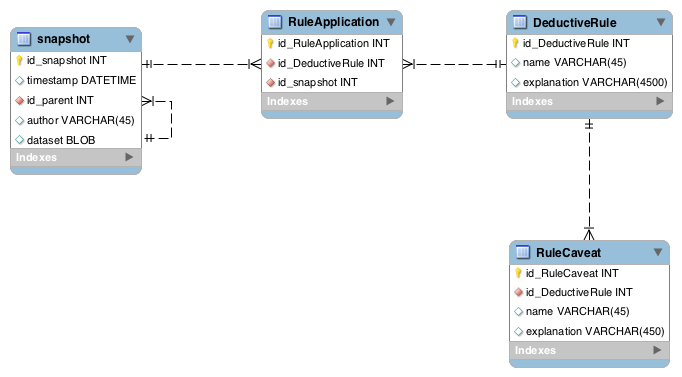
\includegraphics[scale=0.5]{figures/deduction_model}
  \caption{A relational model of a snapshot and deductions.}
  \label{deduction_model}
\end{figure}



\chapter{Sparky extension for reproducible spectral analysis}
\label{sec_sparky_extension}

\begin{center}
  \textit{The best way to predict the future is to invent it.}

 - Alan Kay
\end{center}


Sparky \cite{sparky} is a popular program for interactive peak picking,
GSS construction, and chemical shift assignment.  Sparky is implemented 
with a C++ core, and Python extensions.  It is designed with
extensibility in mind, with a convenient Python API through which 
the core data model can be accessed.  The
extensions are also able to augment the user interface with additional
controls, as well as script common operations, and provide extra algorithms
for analysis.  Since Python is a full-featured programming language, 
it is also possible to interact with the filesystem, loading and dumping
data if necessary, as well as calling additional third-party tools.

The extension is intended to help the spectroscopist to capture the 
missing data of analysis: intermediate primary data, extraneous
data, deductive meta data, and notes.  The general approach is to augment
Sparky's data model and user interface with new functionality.



\section{Getting started with Sparky}

\subsection{Getting Sparky}
A Sparky version including the reproducibility extension can be found at
\url{https://github.com/mattfenwick/SparkyExtensions/releases}.  Simply 
choose the latest version of the correct platform, download it, untar and 
unzip it, and run the sparky executable (in Contents/Resources/bin in the
Mac version, and bin/ in the Linux version).

\subsection{Dependencies}
The reproducibility extension requires a working git installation in order
to capture snapshots.  git is a freely available tool for version control,
and may be found at \url{http://git-scm.com/downloads}.
git works with local files -- no setup of remote hosts is required.
A git client (a list of which may be found at \url{http://git-scm.com/downloads/guis})
is a useful tool to help view and manage a git repository.  A simple,
cross-platform git client that I have used successfully is "giteye",
which may be found at \url{http://www.collab.net/giteyeapp}.

\subsection{Sparky manual}
Sparky manuals, which cover the complete use of the program and its many
features in depth, may be found at 
\url{http://www.cgl.ucsf.edu/home/sparky/manual/} and 
\url{http://pine.nmrfam.wisc.edu/PINE-SPARKY/}.

\subsection{Sparky keyboard shortcuts}
While all Sparky functionality can be accessed through its point-and-click
menu interface, it is far faster to use the keyboard shortcuts, especially
for common tasks.  The most useful of these shortcuts are covered in Table
\ref{sparky_shortcuts}.

\subsection{Sparky extensions}
Extensions are accessible through the "extensions" pull-down menu,
as shown in Figure \ref{sparky_extensions}.
Additionally, the reproducibility extension is accessible through
the "re" shortcut (see Figure \ref{sparky_reproducibility}),
and the "rg" shortcut brings up the group editor.



\section{Concepts}
Automated algorithms do not usually produce perfect results in NMR analysis.
Automated peak picking,
GSS construction, and GSS-residue assignment need manual validation and
correction.  These manual modifications are inherently difficult, tedious,
and error-prone because they are the most complicated to correctly analyze.
However, correctly analyzing them has an important impact on the quality
of the final result.
The main goal of this extension is to facilitate reproducibility
by capturing the entire analysis process, including manual modifications.

The process of manual analysis is composed of a series of discrete steps.
At each step, a deductive rule is applied to the data set, producing a
modified new data set.  Thus, for each rule, knowing the context is important:
it allows one to determine how appropriate the application of a specific rule
is, as well as what the results should be, and to determine whether the 
results are consistent with expectations.

\subsection{GSS and resonance}
Sparky's data model is shown in Figure \ref{sparky_model}.  It includes 
entities for spectra, peaks, resonances, GSS, atoms, and molecules, among
others.  Sparky does not natively distinguish between a GSS (generic spin 
system) and a residue, nor between a resonance and an atom.

Both GSSs and resonances have been implemented in the extension, based 
on the CCPN model \cite{ccpn}.

\subsection{Extraneous data}
In standard analysis, false positive peaks (picked as true peaks initially,
but later determined to be noise or artifactual) and false positive spin 
systems (not assigned to any residue) are typically deleted and/or ignored.
In this extension, \textbf{data is never deleted}.  Such results are kept,
since they have valuable information content, even if they are not used for
the immediate purpose of the analysis process (be it structure or dynamics
determination).  These results are kept by, instead of deleting them, 
explicitly marking them as not of interest, and placed in a different
category.

\subsection{Snapshots}
Snapshots of intermediate states during analysis are used to enable rehashing
of the deductive process.  In general, by capturing a snapshot of the data set
each time a deductive rule is applied, the context of each manual modification
is captured.

An additional benefit of capturing snapshots is that they allow one to go 
backward in time.  This is useful for understanding what happened and
why, but is also useful for fixing mistakes and accidents -- this is
important because Sparky does not really have the capability to undo
changes.  If a datum is accidentally gets changed: 1) it may not even
be noticed, and 2) it is probably impossible to easily restore.  By capturing
snapshots, both of these problems are trivially solved.

\subsection{Deductive reasoning}
Capturing the deductive rules applied during the process of manual assignment
provides semantic information about what is being done and why.  This makes it
far more meaningful to examine the sequence of snapshots of an analysis
process and determine the context.



\section{Project setup}
From the terminal, create an empty directory and "cd" into it.
Intialize it as an empty git repository and create the Sparky directory
structure with the following terminal commands:
\begin{verbatim}
$ git init
$ mkdir Projects/
$ mkdir Save/
$ mkdir Data/
\end{verbatim} 
Make sure to save all spectra files in the "Data/" directory.
When in Sparky, save the project in the "Projects/" directory.
The Sparky .save files will automatically be written into the "Save/"
directory.

Now start Sparky and take care of tedious initial project setup.  This includes:
\begin{itemize}
  \item opening each of the spectra that will be used (using the "fo" shortcut)
  \item setting the contour levels ("ct").  Some nice default setting are
    "15 levels" for both positive and negative contours, and "red-yellow" color
    for positives, along with "blue-green" for negatives
  \item setting the ornament and label sizes ("ot" and "oz")
  \item setting the visible depth
  \item getting the axes in the correct order ("xx" and "xr")
  \item setting the aspect of each spectrum appropriately ("yt")
  \item syncing axes of identical nuclei.  For example, the 1H axes of
    an NHSQC, HNCACB, HN(CO)CACB, HNCO, and C(CO)NH-Tocsy should be synced; 
    similarly, all their 15N axes should be synced as well.  However, the
    13C axis of an HNCACB and an HNCO should not be synced, although the
    13C axis of an HNCACB and a C(CO)NH-Tocsy should by synced
\end{itemize}
Now it is time to take a snapshot of this configuration.

\section{Capturing a snapshot}
Whenever a snapshot is desired, this procedure must be followed:
\begin{itemize}
  \item save the project ("js")
  \item type in the appropriate deductive reason in the "deductive reason used"
    text box, or whatever annotation accurately describes the purpose of the 
    snapshot
  \item click the "make snapshot" button
\end{itemize}
This will use git to create a new snapshot.  At any time, the contents of
the git repo can be examined using the terminal and the file browser.  Git
supports many features for examining and manipulating history.  These may
all be accessed from the terminal.

% TODO does this paragraph make any sense?
Snapshots provide a record of the process of analysis.  By capturing snapshots
at appropriate intervals, effective perusal of the process at a later date is
enabled.  A more immediate benefit is the ability undo mistakes, which is 
important because most mistakes can not be undone using Sparky.
In general, it is necessary to capture a snapshot immediately after
running an automated tool and before making any manual modifications.  During
manual analysis, capturing a snapshot after each focused sub-goal is necessary.



\section{Reproducible backbone assignment tutorial}
There is a nice tutorial and dataset in Sparky format at 
\url{http://www.nmr.chem.uu.nl/~abonvin/tutorials/Assignment-Data/assignment.html}.
It includes the NHSQC, HNCACB, and HN(CO)CACB of a small protein -- enough
to carry out sequential backbone assignments.
This section will show how to reproducibly make these chemical shift
assignments.

\subsection{NHSQC peak picking}
Use standard Sparky facilities to peak pick your NHSQC spectrum.
First, make sure to set the contour levels high enough that few noise and 
artifact peaks will be picked, but low enough that most true signal peaks
will be picked.

\subsection{NHSQC cleanup: signal/noise/artifact identification}
Some of the peaks Sparky found will turn out to be noise or artifact peaks.
\textbf{Do not delete peaks, ever, for any reason!}  Instead,
when peaks are identified as such, select them and press the "Set selected 
peaks to noise" or "Set selected peaks to artifact" button, as necessary.
Peaks must not be assigned when setting them to noise or artifact.

Sparky will not find all true peaks.  Whenever a true signal is found 
unpicked, simply pick the peak manually by switching the cursor mode to 
"find/add peak" and using "pc" to center the peaks after they have been
picked.

Overlapped peaks are also a problem.  They may cause too few peaks to be 
picked, or peaks to be picked in a slightly wrong position.  If these errors
can be rectified manually, simply add peaks and move others as necessary.

Either a restricted peak pick (using NHSQC peaks) or a standard peak pick
of the full dimensions should be used to peak pick all other N-H-rooted
spectra (such as the HNCO, HNCACB, CCONH-Tocsy, etc.).

\subsection{GSS initialization}
It is convenient to create one GSS for each NHSQC peak that is or may be
a signal peak.  Select the NHSQC peaks which will be used as GSS roots.  
All signal peaks can be selected using the "select signal peaks" drop-down.
Then press the "create new group for peak" button.

When an NHSQC peak is used to initialize a GSS, the GSS will start off
with two resonances: one for the H, and one for the N.

\subsection{GSS construction}
Open the peak-GSS assignment dialog by pressing the "Open peak-GSS dialog"
at the bottom of the reproducibility window.

Now set up the parameters by choosing the spectra from which peaks will
be used as GSS roots (typically the NHSQC) and that which has the peaks to
be assigned.  Make sure the desired dimensions are matched and set the 
tolerances appropriately; I typically use 0.2 PPM for a 15N axis and 0.02 PPM
for a 1H axis but this can vary based on the alignment between spectra.
Finally, select all the peaks in the "from" spectrum that should be used;
you can select all signal peaks using the "select signal peaks" drop-down.

The way that GSS construction works is that for each peak in the "from"
spectrum, all peaks in the "to" spectrum within the tolerances will be
assigned to the same GSS as the "from" peak.  Peaks in the "to" spectrum that
match 0 "from" peaks will not be assigned to any GSS; those that match more
than 1 peak will also not be assigned, but a warning will be generated in
the shell, allowing manual resolution.

Matching requires that some subset of the spectral dimensions match.  Using
an NHSQC and an HNCACB, the H and the N dimensions match.  The resonance
assignments of the peak cross sections will be carried over for matching dimensions,
and new resonances will be created for the C dimension.

\subsection{Peak cross section to resonance assignment}
A resonance is assigned to each cross section of each group which is in a GSS.
If a peak cross section has a unique chemical shift value within a GSS, it will
be the only one assigned to that resonance; if multiple cross sections share 
the same or similar chemical shift value, they will be assigned to the same
resonance.  This reflects the fundamental NMR property that an atom resonates
at the same frequency across spectra. 

Peak cross section to resonance assignment can fail in two cases, and these
can be resolved by manually modifying the assignments to resonances.

First, when the chemical shifts between the peak cross sections do not match
within the tolerances, multiple resonances are created.  These can be merged
using the built-in Sparky assignment tools by changing the assignment of one
peak cross section to match the other.
Second, in the case of overlap, a single resonance is created when there
should actually be multiple resonances.  This can also be resolved using 
the built-in Sparky assignment tools, by simply changing the assignment of
one peak dimention to a fresh resonance id.

\subsection{Changing peak-GSS assignments}
There are two major cases for moving a peak from one GSS to another.
First, for GSS types such as Q and N sidechains, there are usually multiple
peaks in the NHSQC (because of the two protons).  Simply select the appropriate
peaks, choose a GSS id (typically the lowest of the GSS ids of the selected
peaks, just for convenience and consistency) and press the "set groups of
selected peaks" button.
Second, peaks may be assigned to the wrong GSS.  Select the incorrect peaks,
type in the desired GSS id, and press the "set groups of selected peaks" button.

\subsection{Resonance typing}
The types of resonances are assigned using BMRB statistics, GSS typing, 
peak characteristics,
and the pulse sequences of the spectra in which they appear.  For some spectra,
such as the NHSQC, there are relatively few choices: for backbone GSSs,
the resonance types are always amide-H and amide-N.  However, other spectra
have more choices: for the HNCACB, resonances in backbone GSSs in the C
dimension can be CA, CA(i-1), CB, or CB(i-1).

There are two ways to assign resonance types.  First, each resonance assigned
to a peak's cross sections a peak may be assigned at once.  The possibilities
for these resonance typings are called "peaktypes" and depend on the pulse 
sequence of the spectrum in which the peak is found.
This can be done using "assign peaktype" drop-down menu.  Select the correct
spectrum, which will bring up a list of possible peaktypes which may be found
in that spectrum.  Make sure to set the dimension order properly.

The second way is to assign resonance types individually.  This can be done 
using the keyboard shortcut "rg" to bring up a group/resonance editor
(see Figure \ref{sparky_reproducibility}).  Clicking on a group will allow
for editing of group assignments, while clicking on a resonance allows for
resonance typing.

Ambiguous resonance typings are also supported.  Common examples include
CA/CA(i-1), HA2/HA3 (Glycine), HB2/HB3 (many amino acids), and QB (Alanine).

\subsection{GSS typing, sequential, and sequence-specific assignment}
GSSs are assigned types based on BMRB statistics, the presence or absence of
characteristics resonance types, and possibly also based on the assignments 
of linked GSSs.
GSS types for H-N-rooted GSSs include backbone types for each of the 20 
standard amino acids, as well as sidechain types for Q, N, R, W, and K.

Sequential GSS assignments are identified based on overlapping compatible
resonances between GSSs: for example, a GSS with a CA at 58.32 PPM and a CB
at 30.27 PPM, and a second GSS with a CA(i-1) at 58.21 and a CB(i-1) at 30.41:
these GSSs have overlapping compatible resonances and can be sequentially
assigned.
It is not necessary that resonance types are unambiguously assigned before
doing sequential GSS assignments: if it is unclear whether a resonance is a
CA or CA(i-1), this may be assigned simultaneously as the sequential assignment
is made, if it is consistent with the overlap from the other GSS.

Additionally, sequential GSS assignment can lead to the picking of additional
peaks, or the resolution of GSS overlap, if such picking and/or resolution
leads to consistent and compatible overlap with another GSS.
GSSs are assigned to residues on the basis of GSS typing, sequential GSS
assignments, and the primary sequence.

GSS assignment is accomplished using the "group editor" dialog by clicking on
the appropriate group.  This will bring up a dialog which allows typing,
sequential assignment, and sequence-specific assignment.



\section{Pitfalls}
Sparky's data model was extended to support reproducible analysis.
However, it is possible to circumvent the extension's model and assign peaks
and resonances differently. If care is not taken when doing so, the data
may be incompatible with the extension.

\section{Creating an NMR-Star file}
While the data is stored as standard Sparky-formatted files in a git repository
during analysis for convenience, after analysis is complete, the project
may be converted to a single NMR-Star file, containing the complete history
of the project.  This conversion may be accomplished using a tool which
automatically extracts each snapshot version from the git repository, 
parses the snapshot into a data structure,
calculates semantic diffs between successive snapshots, 
and finally generates an NMR-Star file containing the data.

 

% tables
\clearpage
\section{Tables}

\begin{table}[h]
  \begin{tabular}{ | c | c | }
    \hline
    shortcut    &   effect      \\  \hline
    ct      &       \\  \hline
    vt      &       \\  \hline
    yt      &       \\  \hline
    pc      &       \\  \hline
    aD      &       \\  \hline
    pa      &       \\  \hline
    re      &  open reproducibility dialog     \\  \hline
    rg      &  open group editor dialog     \\  \hline
    zi      &  zoom in     \\  \hline
    zo      &  zoom out     \\  \hline
    zu      &  move up a plane     \\  \hline
    zd      &  move down a plane     \\  \hline
    ot      &  ornament settings     \\  \hline
    xr      &       \\  \hline
    xx      &       \\  \hline
    jo      &       \\  \hline
    jc      &       \\  \hline
    js      &       \\  \hline
    fo      &       \\  \hline
    py      &  open Python interpreter  \\  \hline
  \end{tabular}
  \caption{Sparky keyboard shortcuts.}
  \label{sparky_shortcuts}
\end{table}



% figures
\clearpage
\section{Figures}

\begin{figure}[h]
  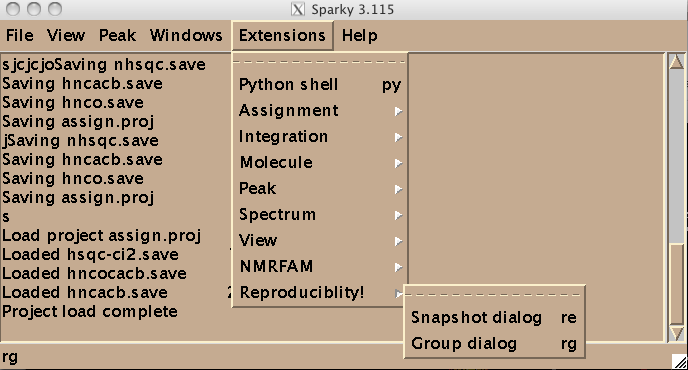
\includegraphics[scale=0.6]{figures/sparky_extensions}
  \caption{The Sparky GUI, showing how to activate the reproducibility
           extension.}
  \label{sparky_extensions}
\end{figure}

\begin{figure}
  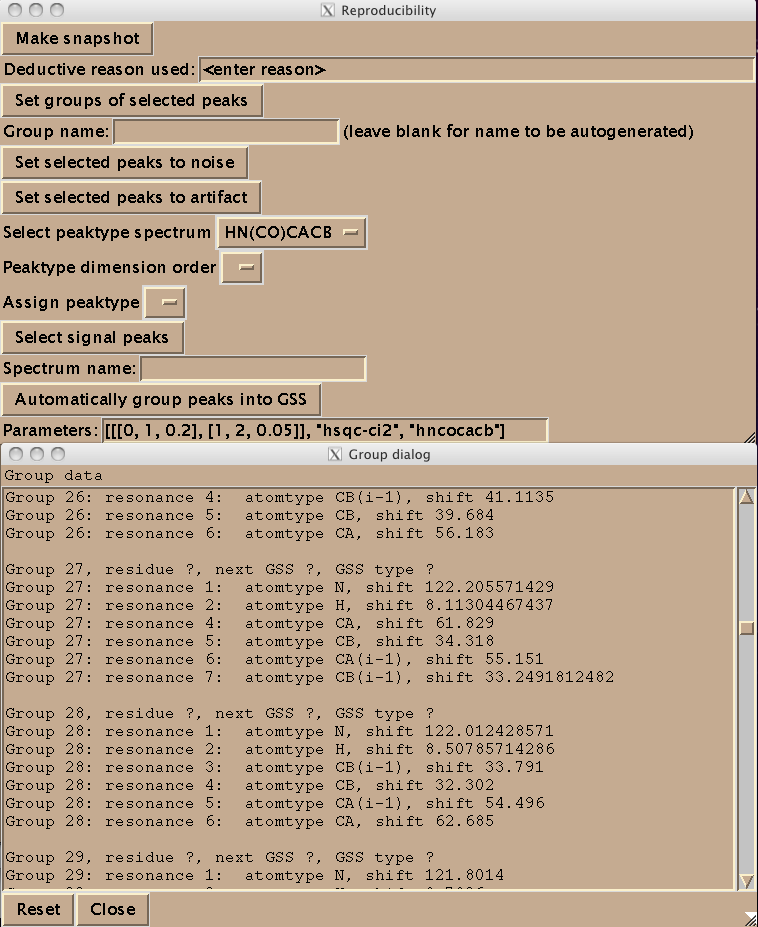
\includegraphics[scale=0.5]{figures/sparky_reproducibility}
  \caption[Two widgets provided by the reproducibility extension.]
          {Two widgets provided by the reproducibility extension.
           The first provides core functionality for making snapshots,
           annotating snapshots, and creating and building GSSs, as
           well as assigning peaktypes.  The second provides functionality
           for displaying, assigning and merging GSSs and resonances.}
  \label{sparky_reproducibility}
\end{figure}

\begin{figure}
  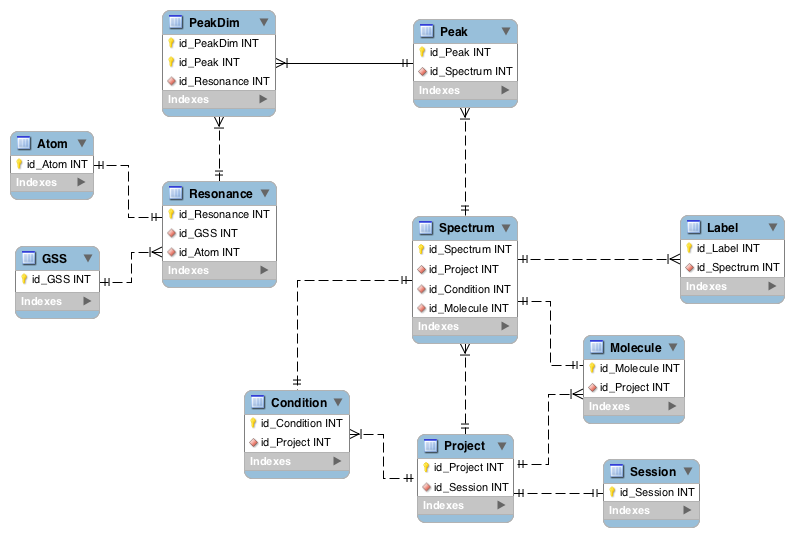
\includegraphics[scale=0.5]{figures/sparky_model}
  \caption[The Sparky data model]
          {The Sparky data model showing the key relationships.
           These data are available from within Sparky extensions.
           The model was created in MySQLWorkbench.}
  \label{sparky_model}
\end{figure}



\chapter{Sparky Extension for Reproducible Spectral Analysis}
\label{sec_sparky_extension}

\begin{center}
  \textit{The best way to predict the future is to invent it.}

 - Alan Kay
\end{center}


Sparky \cite{sparky} is a popular program for interactive peak picking,
GSS construction, and chemical shift assignment.  Sparky is implemented 
with a C++ core, and Python extensions.  It is designed with
extensibility in mind, with a convenient Python interface through which 
the core data model can be accessed.  The
extensions are also able to augment the user interface with additional
controls, as well as script common operations, and provide extra algorithms
for analysis.  Since Python is a full-featured programming language, 
it is also possible to interact with the filesystem, loading and dumping
data if necessary, as well as calling additional third-party tools.

The extension is intended to help the spectroscopist to capture the 
missing data of analysis: intermediate primary data, extraneous
data, deductive meta data, and notes.  The general approach is to augment
Sparky's data model and user interface with new functionality.



\section{Getting started with Sparky}

\subsection*{Getting Sparky}
A Sparky version including the reproducibility extension can be found at
\url{https://github.com/connjur/SparkyExtensions/releases}.  Simply 
choose the latest version of the correct platform, download it, untar and 
unzip it, and run the sparky executable (in Contents/Resources/bin in the
Mac version, and bin/ in the Linux version).

\subsection*{Dependencies}
The reproducibility extension requires a working git installation in order
to capture snapshots.  git is a freely available tool for version control,
and may be found at \url{http://git-scm.com/downloads}.
git works with local files -- no setup of remote hosts is required.
A git client (a list of which may be found at \url{http://git-scm.com/downloads/guis})
is a useful tool to help view and manage a git repository.  A simple,
cross-platform git client that I have used successfully is "giteye",
which may be found at \url{http://www.collab.net/giteyeapp}.

\subsection*{Sparky manual}
Sparky manuals, which cover the complete use of the program and its many
features in depth, may be found at 
\url{http://www.cgl.ucsf.edu/home/sparky/manual/} and 
\url{http://pine.nmrfam.wisc.edu/PINE-SPARKY/}.

\subsection*{Sparky keyboard shortcuts}
While all Sparky functionality can be accessed through its point-and-click
menu interface, it is faster to use the keyboard shortcuts, especially
for common tasks.  The most useful of these shortcuts are covered in Table
\ref{sparky_shortcuts}.

\subsection*{Sparky extensions}
Extensions are accessible through the "extensions" pull-down menu, as shown 
in Figure \ref{sparky_extensions}. The reproducibility extension is also 
accessible through the "re" shortcut (see Figure \ref{sparky_reproducibility}),
and the "rg" shortcut open the group editor.



\section{Concepts}
Automated algorithms do not usually produce perfect results in NMR analysis.
Automated peak picking,
GSS construction, and GSS-residue assignment need manual validation and
correction.  These manual modifications are inherently difficult, tedious,
and error-prone because they are the most complicated to correctly analyze.
However, a correct and complete interpretation is necessary to obtain a 
high-quality final result.
The main goal of this extension is to facilitate reproducibility
by capturing the entire analysis process, including manual modifications.

The process of manual analysis is composed of a series of discrete steps.
At each step, a deductive rule is applied to the data set, producing a
modified new data set.  Thus, for each rule, knowing the context is important:
it allows one to determine how appropriate the application of a specific rule
is, as well as what the results should be, and to determine whether the 
results are consistent with expectations.

\subsection*{GSS and resonance}
Sparky's data model is shown in Figure \ref{sparky_model}.  It includes 
entities for spectra, peaks, resonances, GSS, nuclei, and molecules, among
others.  Sparky does not natively distinguish between a GSS (generic spin 
system) and a residue, nor between a resonance and a nucleus.
GSSs and resonances have been implemented in the extension, based 
on the CCPN model \cite{ccpn}.

\subsection*{Extraneous data}
In standard analysis, false positive peaks (picked as true peaks initially,
but later determined to be noise or artifactual) and false positive spin 
systems (not assigned to any residue) are typically deleted and/or ignored.
In this extension, \textbf{data is never deleted}.  Such results are kept,
since they have valuable information content, even if they are not used for
the immediate purpose of the analysis process (be it structure or dynamics
determination).  These results are kept by explicitly marking them as not of 
interest, and placing them in a different category.

\subsection*{Snapshots}
Snapshots of intermediate states during analysis are used to enable rehashing
of the deductive process.  In general, by capturing a snapshot of the data set
each time a deductive rule is applied, the context of each manual modification
is captured.

An additional benefit of capturing snapshots is that they allow one to go 
backward in time.  This is useful for understanding what happened and
why, but is also useful for fixing mistakes and accidents, which usually 
can not be undone from within Sparky.
If a datum is accidentally changed, it may not even be noticed, and it is 
impossible to easily restore.  Capturing snapshots trivially solves both
of these problems.

\subsection*{Deductive reasoning}
Capturing the deductive rules applied during the process of manual assignment
provides semantic information about what is being done and why.  This makes it
more meaningful to examine the sequence of snapshots of an analysis
process and determine the context.



\section{Project setup}
From the terminal, create an empty directory and "cd" into it.
Intialize it as an empty git repository and create the Sparky directory
structure with the following terminal commands:
\begin{verbatim}
$ git init
$ mkdir Projects/
$ mkdir Save/
$ mkdir Data/
\end{verbatim} 
Make sure to save all spectra files in the "Data/" directory.
When in Sparky, save the project in the "Projects/" directory.
The Sparky .save files will automatically be written into the "Save/"
directory.

Now start Sparky and take care of tedious initial project setup.  This includes:
\begin{itemize}
  \item opening each of the spectra that will be used (using the "fo" shortcut)
  \item setting the contour levels ("ct").  Some nice default setting are
    "15 levels" for both positive and negative contours, and "red-yellow" color
    for positives, along with "blue-green" for negatives
  \item setting the ornament and label sizes ("ot" and "oz")
  \item setting the visible depth
  \item getting the axes in the correct order ("xx" and "xr")
  \item setting the aspect of each spectrum appropriately ("yt")
  \item syncing axes of identical nuclei.  For example, the 1H axes of
    an NHSQC, HNCACB, HN(CO)CACB, HNCO, and C(CO)NH-TOCSY should be synced; 
    similarly, all their 15N axes should be synced as well.  However, the
    13C axis of an HNCACB and an HNCO should not be synced, although the
    13C axis of an HNCACB and a C(CO)NH-TOCSY should by synced
\end{itemize}
Now it is time to take a snapshot of this configuration.


\section{Capturing a snapshot}
Whenever a snapshot is desired, this procedure must be followed:
\begin{itemize}
  \item save the project ("js")
  \item type in the appropriate deductive reason in the "deductive reason used"
    text box, or whatever annotation accurately describes the purpose of the 
    snapshot
  \item click the "make snapshot" button
\end{itemize}
This will use git to create a new snapshot.  At any time, the contents of
the git repo can be examined using the terminal and the file browser.  Git
supports many features for examining and manipulating history.  These may
all be accessed from the terminal or from a git client program.
Snapshots should be captured immediately after running an automated tool and 
before making any manual modifications.  During manual analysis, snapshots 
should be captured after each focused sub-goal is completed.



\section{Reproducible backbone assignment tutorial}
A a nice tutorial and dataset in Sparky format may be found at 
\url{http://www.nmr.chem.uu.nl/~abonvin/tutorials/Assignment-Data/assignment.html}.
It includes the NHSQC, HNCACB, and HN(CO)CACB spectra of a small protein,
providing enough data to carry out sequential backbone assignments.
This section will show how to reproducibly make these chemical shift
assignments.

\subsection*{NHSQC peak picking}
Use standard Sparky facilities to peak pick your NHSQC spectrum.
Set the contour levels high enough that few noise and 
artifact peaks will be picked, but low enough that most true signal peaks
will be picked.

\subsection*{NHSQC cleanup: signal/noise/artifact identification}
Some of the peaks Sparky found will turn out to be noise or artifact peaks.
\textbf{Do not delete peaks, ever, for any reason!}  Instead,
when peaks are identified as such, select them and press the "Set selected 
peaks to noise" or "Set selected peaks to artifact" button, as necessary.
Peaks must not be assigned when setting them to noise or artifact.

Sparky will not find all true peaks.  Whenever a true signal is found 
unpicked, simply pick the peak manually by switching the cursor mode to 
"find/add peak" and using "pc" to center the peaks after they have been
picked.

Overlapped peaks are also a problem.  They may cause too few peaks to be 
picked, or peaks to be picked in a slightly wrong position.  If these errors
can be rectified manually, simply add peaks and move others as necessary.

Either a restricted peak pick (using NHSQC peaks) or a standard peak pick
of the full dimensions should be used to peak pick all other N-H-rooted
spectra (such as the HNCO, HNCACB, CCONH-TOCSY, etc.).

\subsection*{GSS initialization}
It is convenient to create one GSS for each NHSQC peak that is or may be
a signal peak.  Select the NHSQC peaks which will be used as GSS roots.  
All signal peaks can be selected using the "select signal peaks" drop-down.
Then press the "create new group for peak" button.

When an NHSQC peak is used to initialize a GSS, the GSS will start off
with two resonances: one for the H, and one for the N.

\subsection*{GSS construction}
Open the peak-GSS assignment dialog by pressing the "Open peak-GSS dialog"
at the bottom of the reproducibility window.

Now set up the parameters by choosing the spectra from which peaks will
be used as GSS roots (typically the NHSQC) and that which has the peaks to
be assigned.  Make sure the desired dimensions are matched and set the 
tolerances appropriately; I typically use 0.2 PPM for a 15N axis and 0.02 PPM
for a 1H axis but this can vary based on the alignment between spectra.
Finally, select all the peaks in the "from" spectrum that should be used;
you can select all signal peaks using the "select signal peaks" drop-down.

In GSS construction, for each peak in the "from"
spectrum, all peaks in the "to" spectrum within the tolerances will be
assigned to the same GSS as the "from" peak.  Peaks in the "to" spectrum that
match 0 "from" peaks will not be assigned to any GSS; those that match more
than 1 peak will also not be assigned, but a warning will be generated in
the shell, allowing manual resolution.

Matching requires that some subset of the spectral dimensions match.  Using
an NHSQC and an HNCACB, the H and the N dimensions match.  The resonance
assignments of the peak cross sections will be carried over for matching dimensions,
and new resonances will be created for the C dimension.

\subsection*{Peak cross section to resonance assignment}
A resonance is assigned to each cross section of each peak which is in a GSS.
If a peak cross section has a unique chemical shift value within a GSS, it will
be the only one assigned to that resonance; if multiple cross sections share 
the same or similar chemical shift value, they will be assigned to the same
resonance.  This reflects the NMR property that a nucleus resonates
at a characteristic frequency across spectra.

Peak cross section to resonance assignment can fail in two cases, and these
can be resolved by manually modifying the assignments to resonances.
First, when the chemical shifts between the peak cross sections do not match
within the tolerances, multiple resonances are created.  These can be merged
using the built-in Sparky assignment tools by changing the assignment of one
peak cross section to match the other.
Second, in the case of overlap, a single resonance is created when there
should actually be multiple resonances.  This can also be resolved using 
the built-in Sparky assignment tools, by simply changing the assignment of
one peak dimention to a fresh resonance id.

\subsection*{Changing peak-GSS assignments}
There are two major cases for moving a peak from one GSS to another.
First, for GSS types such as Q and N sidechains, there are usually multiple
peaks in the NHSQC (because of the two protons).  Select the appropriate
peaks, choose a GSS id (typically the lowest of the GSS ids of the selected
peaks, just for convenience and consistency) and press the "set groups of
selected peaks" button.
Second, peaks may be assigned to the wrong GSS.  Select the incorrect peaks,
type in the desired GSS id, and press the "set groups of selected peaks" button.

\subsection*{Resonance typing}
The types of resonances are assigned using BMRB statistics, GSS typing, 
peak characteristics,
and the pulse sequences of the spectra in which they appear.  For some spectra,
such as the NHSQC, there are relatively few choices: for backbone GSSs,
the resonance types are always amide-H and amide-N.  However, other spectra
have more choices: for the HNCACB, resonances in backbone GSSs in the C
dimension can be CA, CA(i-1), CB, or CB(i-1).

There are two ways to assign resonance types.  First, each resonance assigned
to a peak's cross sections may be assigned at once.  The possibilities
for these resonance typings are called "peaktypes" and depend on the pulse 
sequence of the spectrum in which the peak is found.
This can be done using "assign peaktype" drop-down menu.  Select the correct
spectrum, which will bring up a list of possible peaktypes which may be found
in that spectrum.  Make sure to set the dimension order properly.

The second way is to assign resonance types individually.  This can be done 
using the keyboard shortcut "rg" to bring up a group/resonance editor
(see Figure \ref{sparky_reproducibility}).  Clicking on a group will allow
for editing of group assignments, while clicking on a resonance allows for
resonance typing.

Ambiguous resonance typings are also supported.  Common examples include
CA/CA(i-1), HA2/HA3 (glycine), HB2/HB3 (many amino acids), and QB (alanine).

\subsection*{GSS typing, sequential, and sequence-specific assignment}
GSSs are assigned types based on BMRB statistics, the presence or absence of
characteristics resonance types, and possibly also based on the assignments 
of linked GSSs.
GSS types for H-N-rooted GSSs include backbone types for each of the 20 
standard amino acids, as well as sidechain types for Q, N, R, W, and K.

Sequential GSS assignments are identified based on overlapping compatible
resonances between GSSs: for example, a GSS with a CA at 58.32 PPM and a CB
at 30.27 PPM, and a second GSS with a CA(i-1) at 58.21 and a CB(i-1) at 30.41:
these GSSs have overlapping compatible resonances and can be sequentially
assigned.
It is not necessary that resonance types are unambiguously assigned before
doing sequential GSS assignments: if it is unclear whether a resonance is a
CA or CA(i-1), this may be assigned simultaneously as the sequential assignment
is made, if it is consistent with the overlap from the other GSS.

Additionally, sequential GSS assignment can lead to the picking of additional
peaks, or the resolution of GSS overlap, if such picking and/or resolution
leads to consistent and compatible overlap with another GSS.
GSSs are assigned to residues on the basis of GSS typing, sequential GSS
assignments, and the primary sequence.

GSS assignment is accomplished using the "group editor" dialog by clicking on
the appropriate group.  This will bring up a dialog which allows typing,
sequential assignment, and sequence-specific assignment.



\section{Pitfalls}
Sparky's data model was extended to support reproducible analysis.
However, it is possible to circumvent the extension's model and assign peaks
and resonances differently. If care is not taken when doing so, the data
may be incompatible with the extension.



\section{Creating an NMR-STAR file}
While the data is stored as standard Sparky-formatted files in a git repository
during analysis for convenience, after analysis is complete, the project
may be converted to a single NMR-STAR file, containing the complete history
of the project.  This conversion may be accomplished using the code found at
\url{https://github.com/CONNJUR/Samp3-extractor}, which extracts each snapshot 
version from the git repository, parses the snapshot into a data structure,
calculates semantic diffs between successive snapshots, 
and finally generates an NMR-STAR file containing the data.

 

% tables
\clearpage
\section{Tables}

\begin{table}[h]
  \begin{tabular}{ | c | c | }
    \hline
    shortcut    &   effect                  \\  \hline
    ct      &  open contour dialog          \\  \hline
    yt      &  open spectrum dialog         \\  \hline
    pc      &  center peak                  \\  \hline
    aD      &  delete peak assignment       \\  \hline
    re      &  open reproducibility dialog  \\  \hline
    rg      &  open group editor dialog     \\  \hline
    ot      &  ornament settings            \\  \hline
    xr      &  roll axes                    \\  \hline
    xx      &  transpose axes               \\  \hline
    jo      &  open project                 \\  \hline
    jc      &  close project                \\  \hline
    js      &  save project                 \\  \hline
    fo      &  open spectrum                \\  \hline
    py      &  open Python interpreter      \\  \hline
  \end{tabular}
  \caption{Important Sparky keyboard shortcuts.}
  \label{sparky_shortcuts}
\end{table}



% figures
\clearpage
\section{Figures}

\begin{figure}[h]
  \includegraphics[scale=0.6]{figures/sparky_extensions}
  \caption{The Sparky interface, showing how to activate the reproducibility
           extension.}
  \label{sparky_extensions}
\end{figure}

\begin{figure}
  \includegraphics[scale=0.5]{figures/sparky_reproducibility}
  \caption[Two widgets provided by the reproducibility extension.]
          {Two widgets provided by the reproducibility extension.
           The first provides core functionality for making snapshots,
           annotating snapshots, and creating and building GSSs, as
           well as assigning peaktypes.  The second provides functionality
           for displaying, assigning and merging GSSs and resonances.}
  \label{sparky_reproducibility}
\end{figure}

\begin{figure}
  \includegraphics[scale=0.5]{figures/sparky_model}
  \caption[The Sparky data model.]
          {The Sparky data model showing the key relationships.
           These data are available from within Sparky extensions.
           The model was created in MySQLWorkbench.}
  \label{sparky_model}
\end{figure}



\chapter{Conclusions}

\begin{center}
  \textit{Dealing with failure is easy: Work hard to improve. Success is also 
    easy to handle: You've solved the wrong problem. Work hard to improve.}

 - Alan Perlis
\end{center}


\section{The significance of NMR as an experimental technique}
While NMR has historically been an important technique for studying biological
molecules at an atomic level, it is neither the only technique for such 
studies, nor is it guaranteed to remain so indefinitely.  Although NMR does
currently enjoy a stranglehold in the area of dynamics and has proven itself
many times over as an effective technique for structural, binding, and metabolomics
studies, I believe that NMR's continued success rests on the ability of the
field to solve the several pressing problems facing it.

These problems are varied in nature: some are inherent, and caused by the 
experimental phenomenon of studying nuclei in large magnets using 
radiofrequency pulses; others find their roots in our approach to 
understanding and analyzing the data.

The ability to isolate pure, high-concentration and stable samples of proteins 
is a prerequisite to carrying out an NMR study.  However, this is not only
difficult, but may be impossible in certain cases given our current techniques
\cite{bellstedt2013resonance}.  Worse still is that even for proteins which
can be studied effectively, it is difficult to ascertain how relevant the 
information obtained is to the protein's actual structure and function in the
complex biological system in which we desire to understand its role.  Thus, 
the challenge facing NMR is how to expand its reach to study additional proteins,
and to study proteins in native conditions.

Large proteins also pose severe problems for effective NMR data collection.  
This is because as molecular size increase, peak widths generally increase as
well; at the same time, the number of peaks increases because there are more
atoms in the molecule.  The result is decreased resolution, increased overlap,
and a decreased signal-noise ratio.  All of these lead to data that is more
difficult or impossible to interpret.  One current approach is to chop large
proteins into several smaller pieces which can be studied independently; the
hope is that the results gained are relevant to the full molecule.  
Progress is also being made in the area of improved pulse sequence design
and labeling schemes \cite{tzeng2012nmr}.  Nevertheless, the problem of molecule
size remains an ongoing challenge facing the field of NMR.

Effectively passing on knowledge to new students, and efficiently such that
they are able to quickly make valuable contributions is a problem of a different
sort.  While resources such as \url{http://www.protein-nmr.org.uk/} and books
such as \cite{hoch1996nmr} and \cite{keeler2013} are incredibly valuable and
helpful tools for learning, the task of learning NMR not only in breadth and
in depth, but also from a practical standpoint, remains a formidable and
time-consuming one.  In my opinion, a major contributor to this problem is 
the means employed for transmission of knowledge, information, and data:
information is often implicitly and transiently communicated, such that it is
not understandable without the appropriate context, nor is it recorded.
Books, websites, data archives, and journal publications are clearly effective
in explicitly transmitting and disseminating information; just as clearly,
these and related media are not used for everything.  Thus, the problem facing
NMR is how to identify and provide the resources necessary for efficiently and
effectively introducing new persons into the field. 

Related to previous problem is fostering an understanding and a means of 
discussing and sharing flaws in our work.  I believe the ability to correctly
recognize and understand problems is a prerequisite for solving them; and that
making progress in the field requires such recognition and solutions.  
Furthermore, I believe that in a collaborative community in which the work of
one individual becomes the basis for the work of another, such as the current
scientific community in which we work, explicitly identifying problems and
open issues is as important as making new discoveries; the cycle of first
identifying, and then solving problems is natural to science.  Therefore, 
the field of NMR must determine how to improve its communication of flaws 
and holes in our research, in order to facilitate the solution of them.


\section{Reproducibility: challenge, opportunity}
The major contribution of this work is substantial progress towards solving
the latter two problems by means of reproducibility.  I have presented 
approaches, models, and applications and techniques of those, all aimed toward
two goals: first, to make both information and its context explicit, by recording
and preserving them; and second, to create a concept, means, and vocabulary for
identifying and communicating issues of NMR data analysis.  While these 
accomplishments only directly help to solve the latter two problems, I believe
they will also help to deal with the former two as well -- reproducibility
leads to improved and robust data analysis, which is a prerequisite for dealing
with the lower quality data collected from large or unstable proteins.


\section{The future of NMR software}
Software is integrated into every phase of the process;
because good software facilitates progress, while bad software restricts it,
software quality plays a major role in determining the quality, speed, and 
robustness of NMR analysis. 
There are two key dimensions for measuring software quality: how well a 
software product meets its users' current needs, and how well it is able to
adapt to meet their future needs.  The ability to easily adapt to meet new 
challenges is what enables fast and cheap innovation; conversely, high
barriers to adapting and building software restrict innovation and prevent
improvements.  While NMR software has achieved incredible results, I believe
it is reaching a crossroads with respect to its adaptability.

If flexibility and adaptability are to be achieved,
a new approach to building scientific software must be adopted, and 
a new understanding of the costs and value of software to NMR, must be 
achieved in order to truly take advantage of the benefits that software can
confer.  These changes are fundamentally different from rewriting software
to be more efficient, or have fewer bugs or more features.  Rather, the
goals must be to create software such that it is simple, obvious, and 
composable.  Such design goals naturally lead to correct, feature-rich, 
adaptable, and maintainable software -- but the converse is not true.  Worse
is that complex, non-composable software, instead of enabling
us, places an upper limit on the problems that can be solved using it.

Connjur is an open source project which provides flexible, composable tools
through data integration.  While it is not expected to solve every software
problem NMR spectroscopists face, I believe the software created by the Connjur
project embodies the principles needed to create effective scientific
software, through its bottom-up design and open source licensing:
the first is the best way we know of for dealing flexibly with changing
requirements, and the second is the best way we know of for explicitly 
transmitting information contained in software tools between individuals.


\section{Final thoughts}
In this current climate of decreased scientific funding levels, and increased
competition for precious grant dollars, it is important to meditate upon the
nature, the future, and the effect on society, of science.
While good science can have a positive impact on individuals and on society 
as a whole, bad science can have a corresponding negative impact.
I therefore hope that the goal of reproducibility is taken seriously by all
scientists, not only as a means of expanding human knowledge more quickly and
with less effort, but also a means to minimize the harm of bad science.
I look forward to science of the highest quality.
% where are we going? how will we get there?




% TODO appendices

% not sure what the difference is between `unsrt` and `ieeetr`
% also see `natbib` for another possible alternative
%\bibliographystyle{unsrt}
\clearpage % apparently necessary to get the table of contents to point to the right page for the references
\addcontentsline{toc}{chapter}{References}
\bibliographystyle{ieeetr}
\bibliography{thesis}

\end{document}

